\chapter{Results and Analysis}
\label{chap:results}
This chapter presents the results and analyses of experiments designed to evaluate the effectiveness of the proposed methodology, which combines different loss functions for semantic segmentation tasks. The objective is to gain insights into this approach's performance and potential advantages compared to baseline models.

The chapter is organized into several sections, presenting the results from distinct perspectives. It begins with \emph{quantitative} and \emph{qualitative results}, offering an in-depth analysis of the proposed method's performance across multiple datasets and evaluation metrics. Subsequent sections analyze the \emph{computation time} and evaluate the feasibility of using a data subset to conserve computational resources and time. The findings of the \emph{ablation study} are also presented to shed light on this aspect further.

\section{Quantitative Results}
\label{sec:quantitative_results}
The section aims to provide a comprehensive understanding of the relationships and patterns observed within the data, shedding light on crucial findings that contribute to answering the research questions. The results are showcased using suitable statistical methods and visual representations, including tables, graphs, and charts. 

The section centers on presenting and analyzing quantitative findings from the final configurations, as outlined in table \ref{tab:final_configuration_list}, excluding the time-based merging strategy. This particular strategy is omitted due to its high computational demand and can be explored in future research.

The results are presented individually for each dataset to promote clarity and coherence. Each dataset section is systematically organized into four dataset subsections
\begin{itemize}[noitemsep]
\item Baseline Performance
\item Overall Performance
\item Discrete Performance
\item Continuous Performance
\end{itemize}
each, excluding \squote{Overall Performance}, corresponds to a specific configuration mentioned above, resulting in nine configurations utilized for model training.

Several configurations undergo multiple training iterations when feasible to provide reliable and robust performance. This practice is specific to the dataset and will be discussed in the relevant chapters. For further analysis, the top three performing configuration runs for each dataset subsection are documented in the appendix under \chapref{chap:supplementary_results}.
%----------------------------------------------------------------------------------------%
%---------------------------------------Medaka Fish--------------------------------------%
%----------------------------------------------------------------------------------------%
\subsection{Medaka Fish}
\label{subsec:medaka_fish}
As outlined in \secref{sec:datasets}, the \ac{MFD} comprises images of the Medaka Fish cardiac system, including four classes, one of which is the background class. This subsection elaborates on the results of the four configurations detailed in \secref{sec:configuration}, specifically configurations 1 through 4, as shown in table \ref{tab:final_configuration_list}. These configurations consist of the baseline, discrete, and continuous merge strategy configurations.
%------------------------------BASELINE PERFORMANCE (Medaka)-----------------------------%
\subsubsection*{Baseline Performance}
Table \ref{tab:baseline_medaka_short} summarizes the baseline results for the \ac{MFD}. Each row represents the average performance by the loss function. This baseline average was created using configuration no. 1 defined in \secref{sec:configuration}. This configuration underwent six training rounds for a reliable performance assessment, leading to the development of 108 models. The final column of the table, \squote{\ac{PPV} vs. \ac{TPR}}, determines whether a scenario presents high precision with low recall or low precision with high recall.

\textbf{Distribution-based Results}\newline
The most notable results were achieved by the \ac{CE} and the \ac{FL}, which performed comparably well on average. The most significant difference, approximately 6\%, was observed in the Bulbus class, which was better predicted by the \ac{FL}. This observation aligns with the findings of \cite{10.1371/journal.pone.0263656}, which reported that the Bulbus class is the most challenging to predict. This outcome is reasonable, as the \ac{FL} is known to down-weight more straightforward examples and focus on more difficult ones.

\textbf{Region-based Results}\newline
\ac{DL} and \ac{TL} performed relatively well, with scores 3.9 and 4.2\% lower than the \ac{CE} and \ac{FL}, respectively. Interestingly, even though the \ac{TL} exhibited just an \ac{IoU} that was 0.3\% lower than the \ac{IoU} of the \ac{CE}, its \ac{TPR} was 2.1\% higher. Among all the loss functions in the distribution and region-based domain, the \ac{TL} demonstrated a higher \ac{TPR} against a typically higher \ac{PPV}, indicating successful implementation, as discussed in \secref{subsec:segmentation_objectives}.

\textbf{Boundary-based Results}\newline
Although the \acf{BL} converged several times during testing, it appeared incapable of converging for this final baseline configuration which can be typical for this type of loss, as it was introduced as an addition rather than intended to serve as a standalone loss function \cite{Kervadec_2021}. In contrast, the \acf{HL} was much more stable. Although some runs did not converge, the average performed reasonably well. 

While initial tests with the original loss defined in \ref{eqn:hausdorff_loss} denoted as $HL$, proposed by \cite{8767031} had a shallow convergence rate for baseline training, this work uses the proposed variant $HL_1$ defined in \ref{eqn:hausdorff_loss_v2} which, after some extensive testing, demonstrated a significantly more robust performance.

\figref{hausdorff_loss_training_curves} illustrates two models trained with the original loss described in \cite{8767031} on image (a) and the improved variant illustrated on image (b) indicating a meaningful implementation.
\begin{figure}[H]%[htbp]
  \centering
  \subfigure[$HL$ loss training curves]{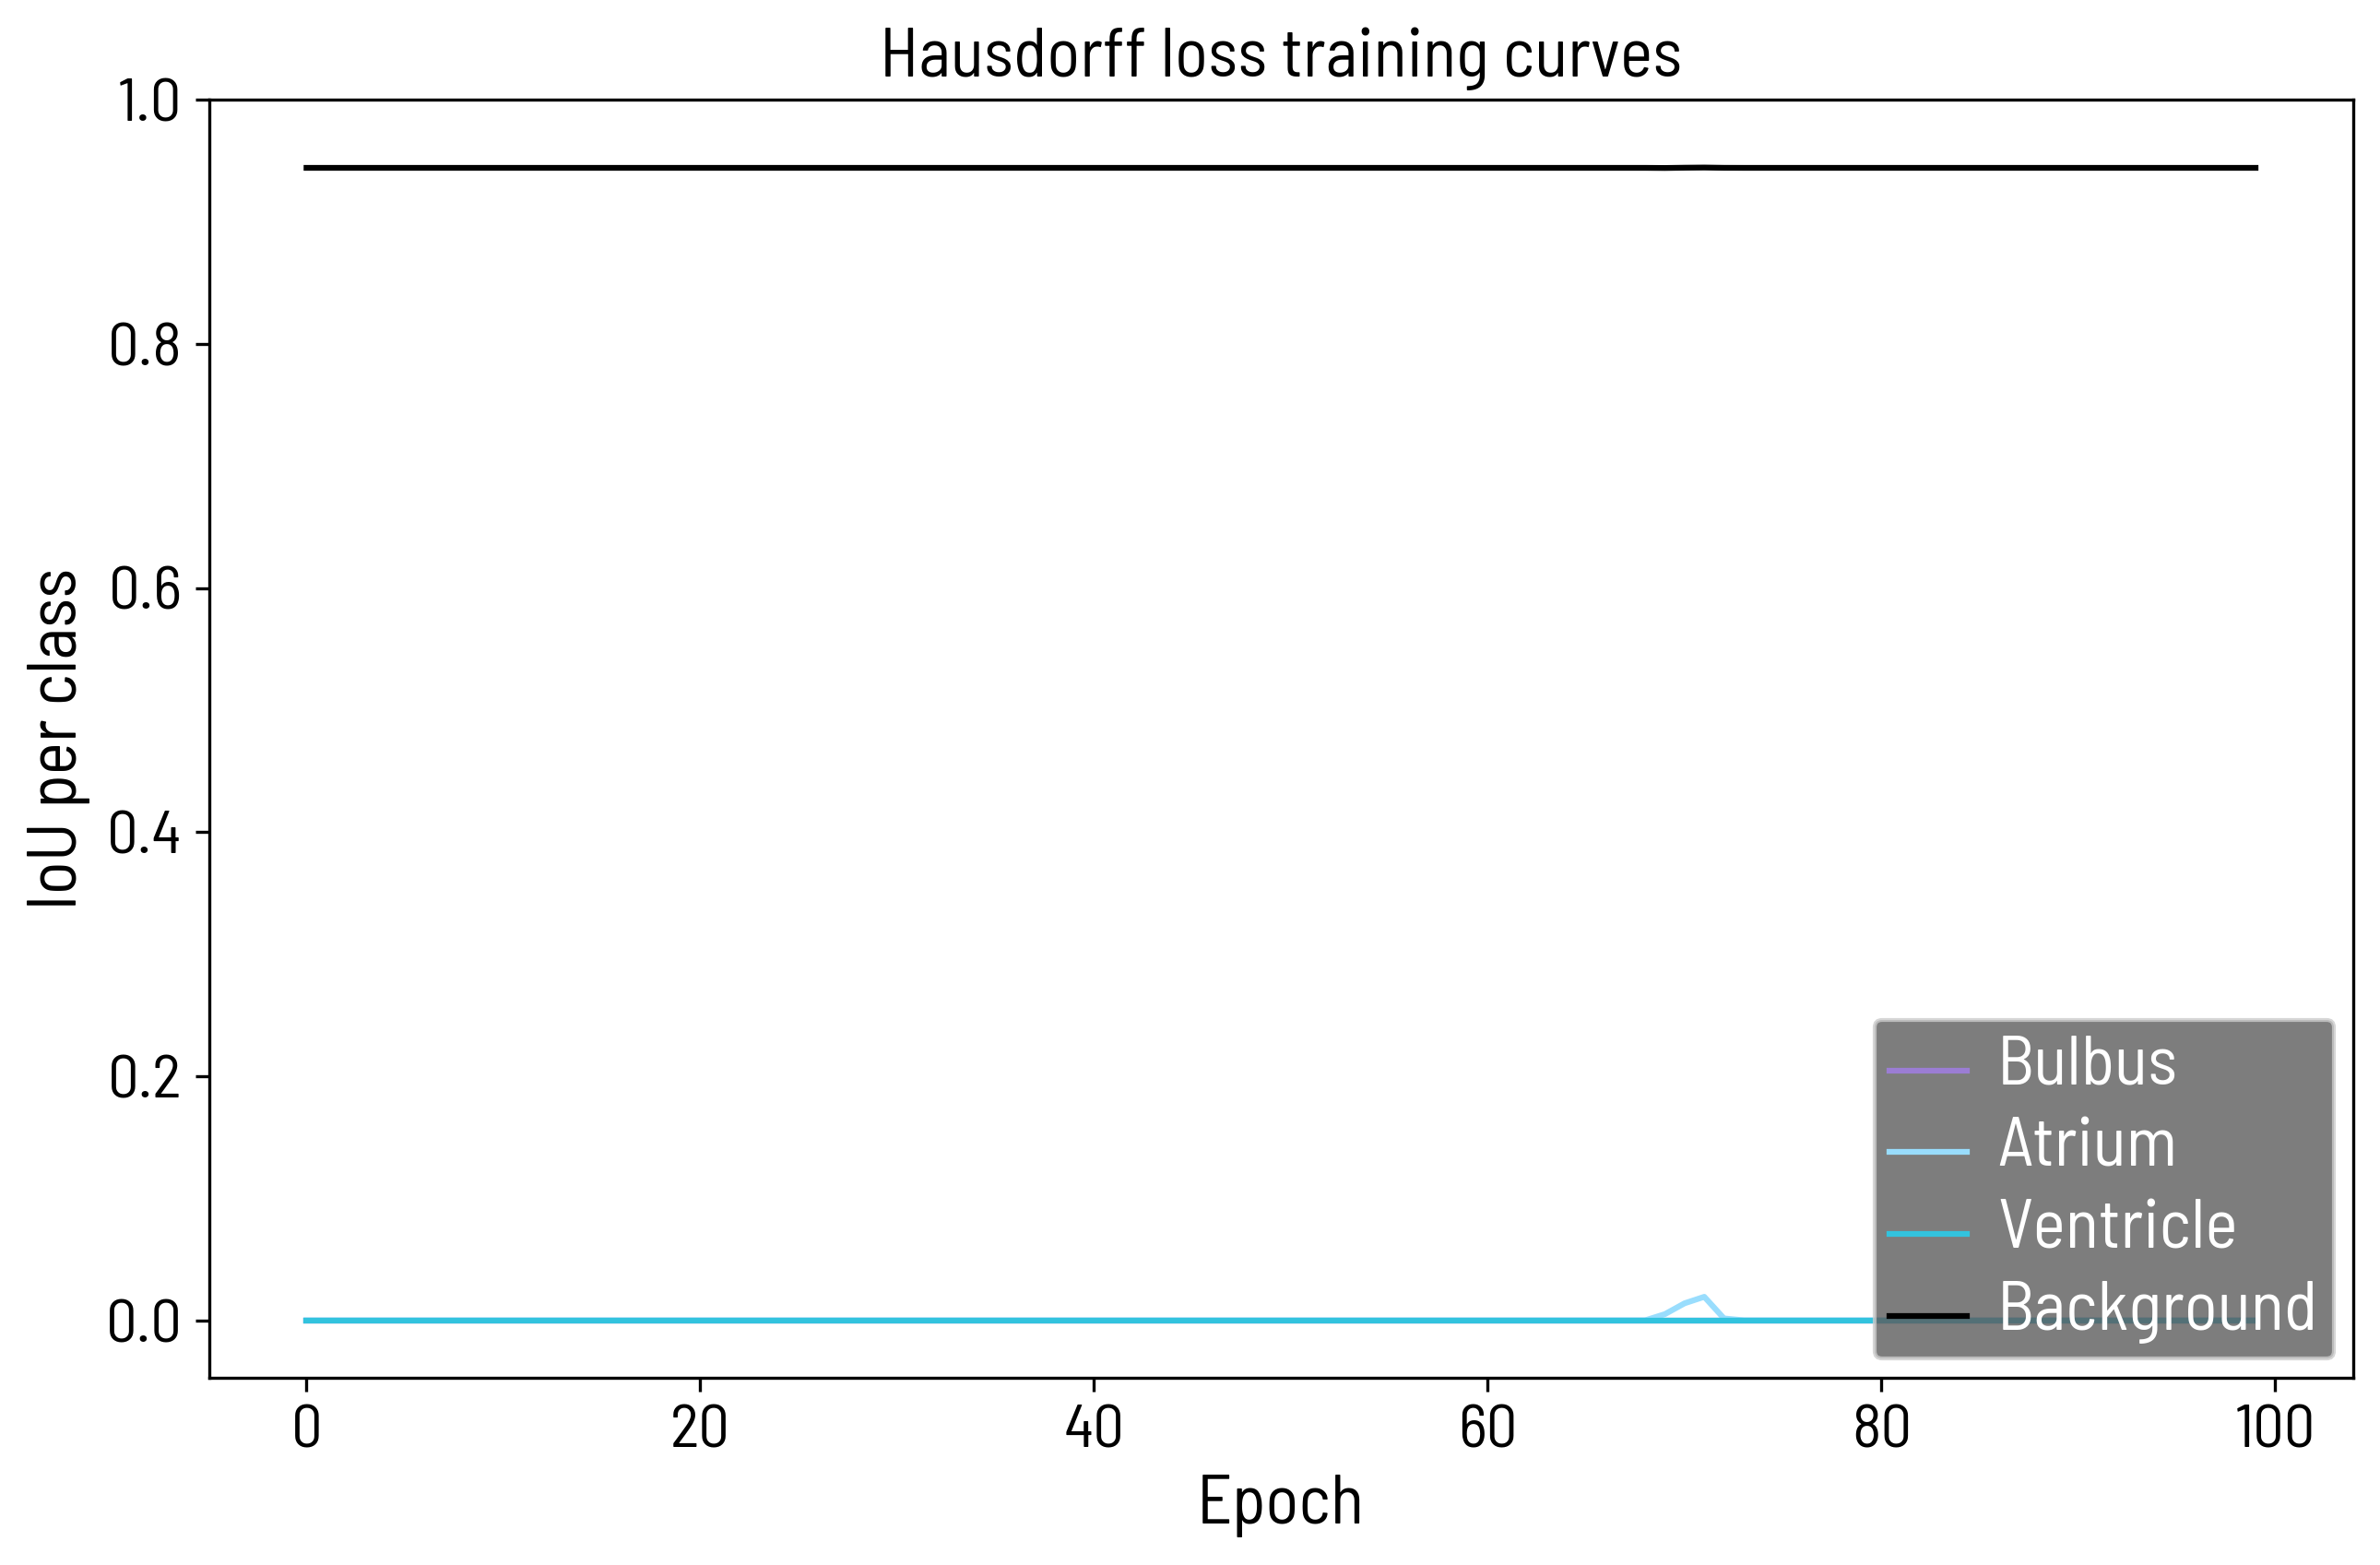
\includegraphics[width=\imgWidthcustom]{images/hausdorff_0_loss_training_curves.png}}
  \subfigure[$HL_1$ loss training curves]{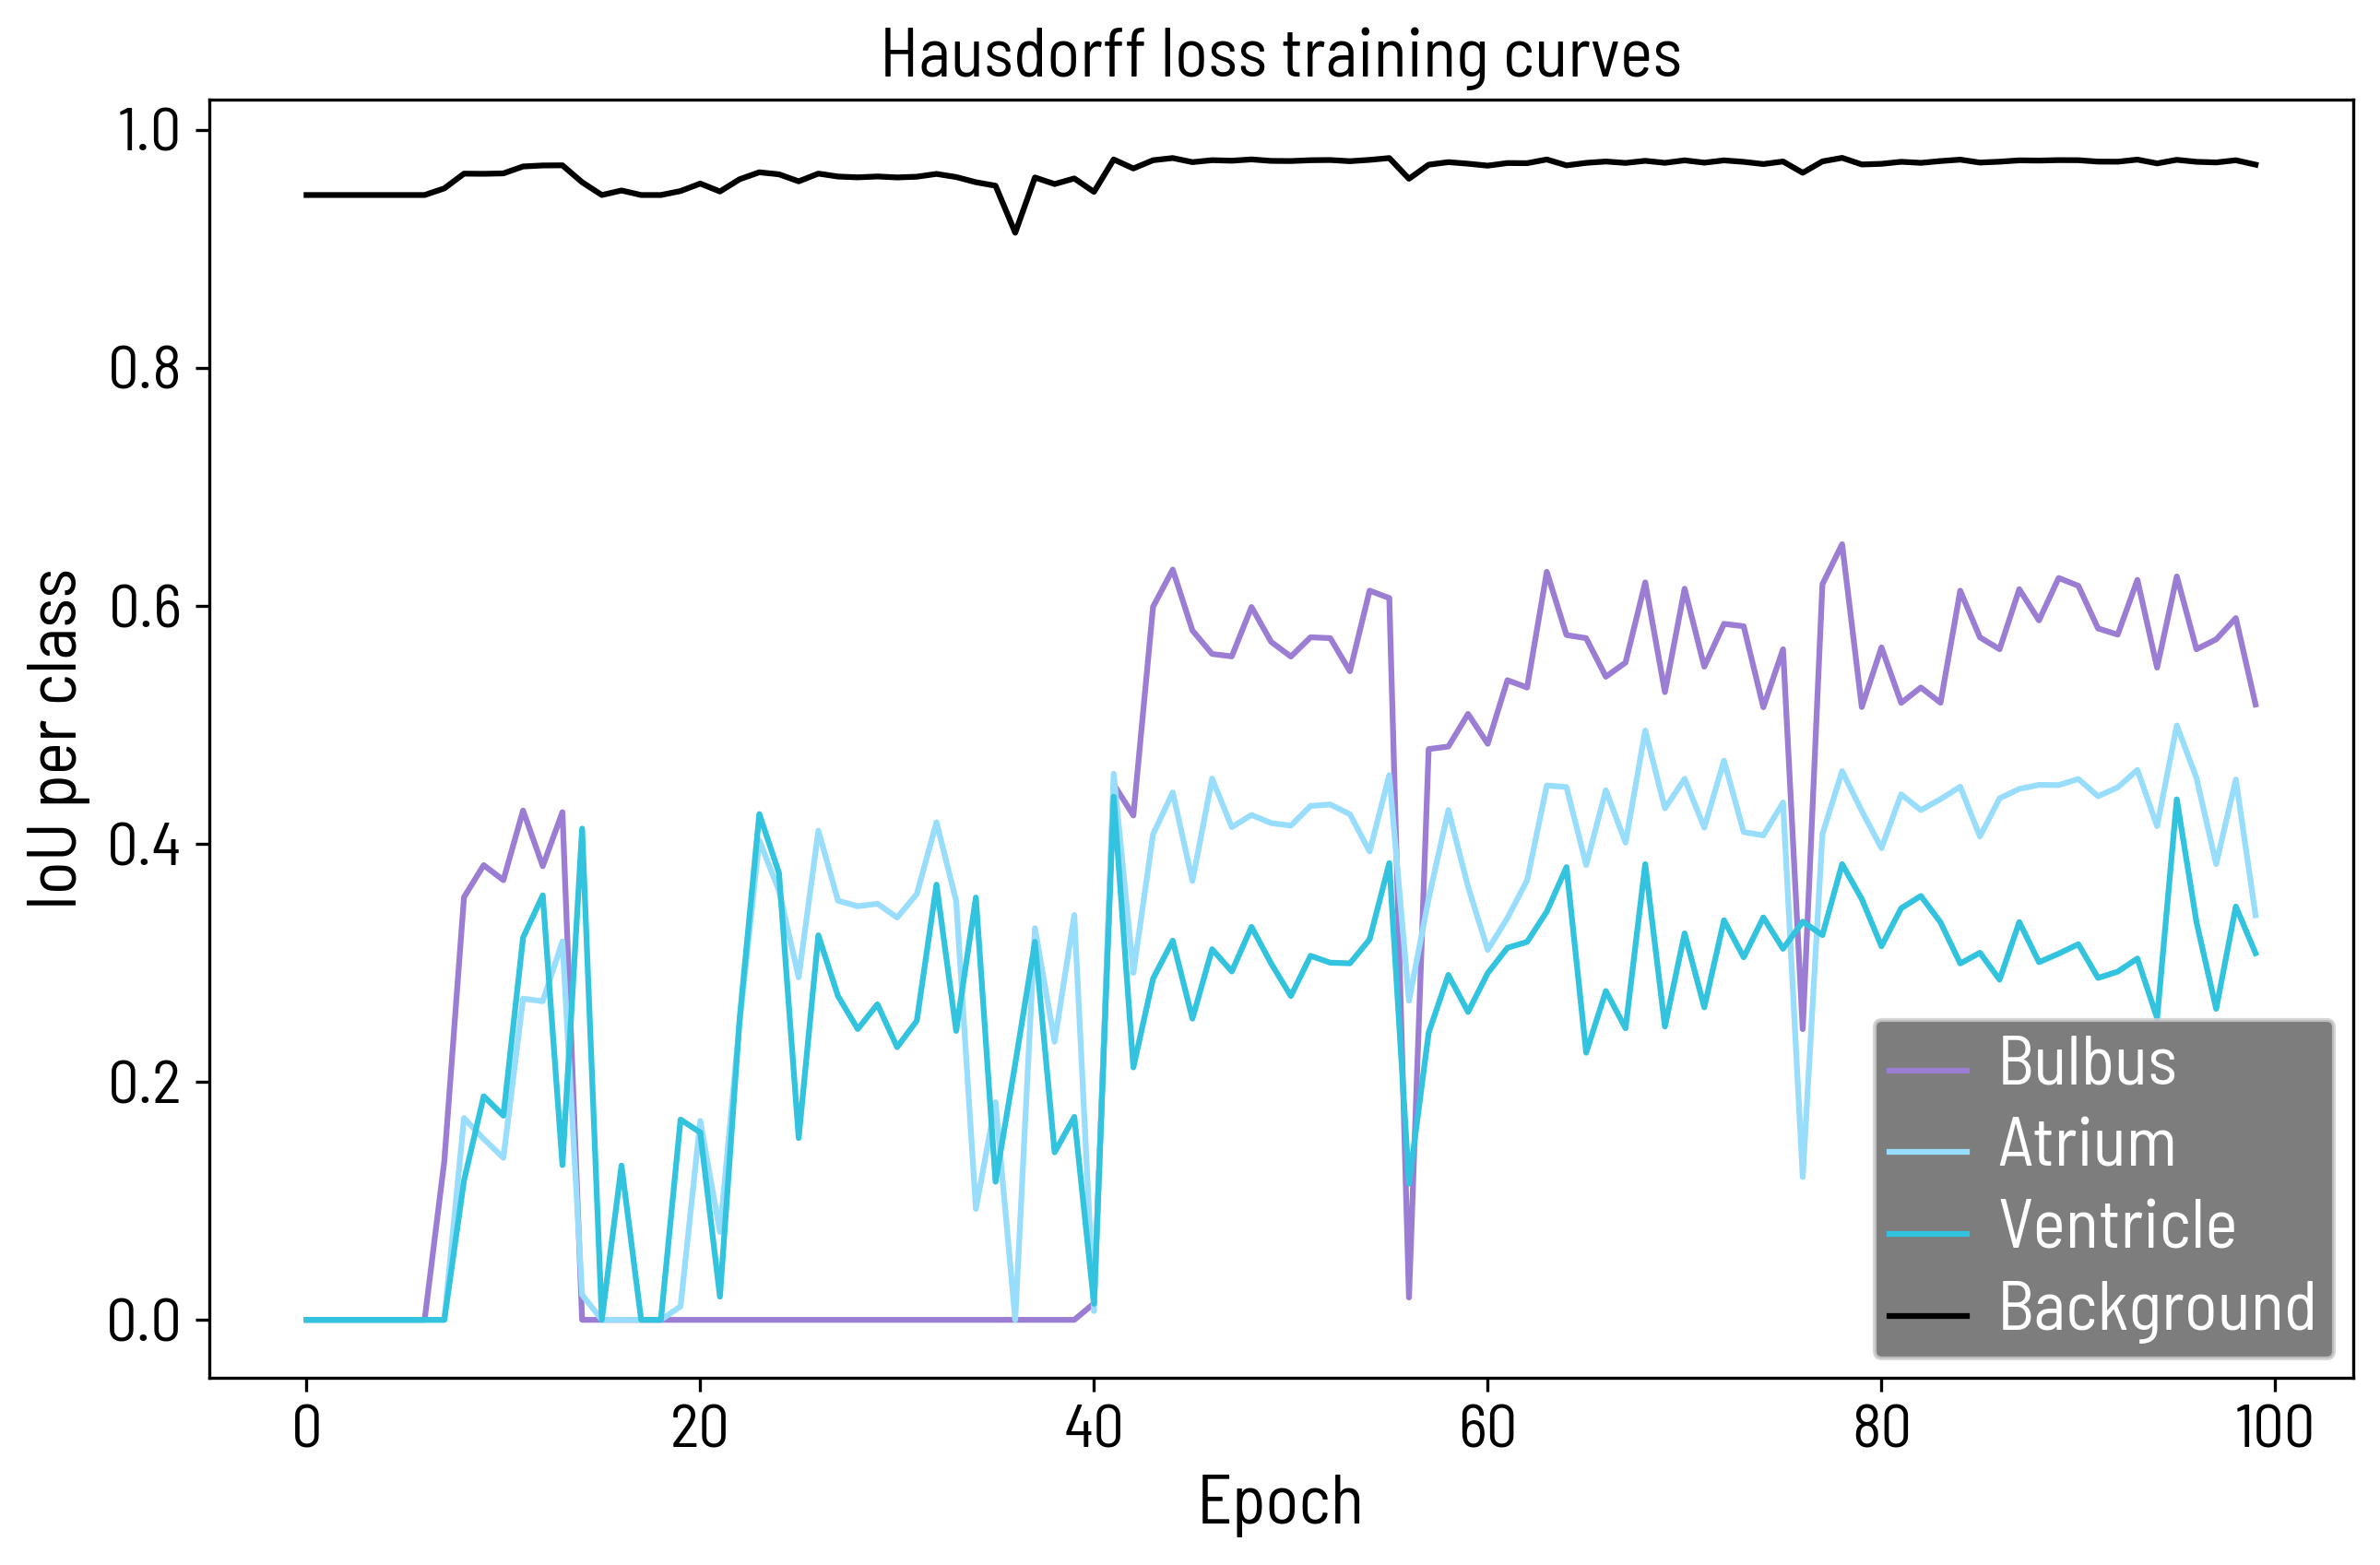
\includegraphics[width=\imgWidthcustom]{images/hausdorff_loss_training_curves.png}}
  \caption[Hausdorff loss training curves]{Learning curves for a model trained with the regular (a) \ac{HL} and enhanced (b) \ac{HL} function. It can be seen that even the difficult Bulbus class starts to improve around epoch 40, showing a drastic performance increase.}
  \label{hausdorff_loss_training_curves}
\end{figure}

% Please add the following required packages to your document preamble:
% \usepackage{graphicx}
% \usepackage[table,xcdraw]{xcolor}
% If you use beamer only pass "xcolor=table" option, i.e. \documentclass[xcolor=table]{beamer}
\begin{table}[H]
  \centering
  \resizebox{\textwidth}{!}{%
  \begin{tabular}{cc|l|l|l|l|l|l|l|l|c|}
  \hline
  \rowcolor[HTML]{000000} 
  \multicolumn{1}{|c|}{\cellcolor[HTML]{000000}{\color[HTML]{FFFFFF} No.}} &
    {\color[HTML]{FFFFFF} Loss type} &
    {\color[HTML]{FFFFFF} Loss} &
    {\color[HTML]{FFFFFF} IoU} &
    {\color[HTML]{FFFFFF} IoU 0} &
    {\color[HTML]{FFFFFF} IoU 1} &
    {\color[HTML]{FFFFFF} IoU 2} &
    {\color[HTML]{FFFFFF} IoU 3} &
    {\color[HTML]{FFFFFF} PPV} &
    {\color[HTML]{FFFFFF} TPR} &
    {\color[HTML]{FFFFFF} PPV vs. TPR} \\ \hline
  \multicolumn{1}{|c|}{\textit{\textbf{1}}} &
    \cellcolor[HTML]{6638B6}{\color[HTML]{FFFFFF} \textit{\textbf{DB}}} &
    \textit{\textbf{CE}} &
    \textit{\textbf{0.672}} &
    \textit{\textbf{0.976}} &
    \textit{\textbf{0.697}} &
    \textit{\textbf{0.530}} &
    \textit{\textbf{0.485}} &
    \textit{\textbf{0.808}} &
    \textit{\textbf{0.766}} &
    \textit{\textbf{PPV}} \\ \hline
  \multicolumn{1}{|c|}{\textit{\textbf{2}}} &
    \cellcolor[HTML]{6638B6}{\color[HTML]{FFFFFF} \textit{\textbf{DB}}} &
    \textit{\textbf{FL}} &
    \textit{\textbf{0.672}} &
    \textit{\textbf{0.976}} &
    \textit{\textbf{0.750}} &
    \textit{\textbf{0.515}} &
    \textit{\textbf{0.445}} &
    \textit{\textbf{0.814}} &
    \textit{\textbf{0.762}} &
    \textit{\textbf{PPV}} \\ \hline
  \multicolumn{1}{|c|}{3} &
    \cellcolor[HTML]{00A9CE}{\color[HTML]{FFFFFF} RB} &
    DL &
    0.633 &
    0.973 &
    0.673 &
    0.465 &
    0.421 &
    0.782 &
    0.725 &
    PPV \\ \hline
  \multicolumn{1}{|c|}{4} &
    \cellcolor[HTML]{00A9CE}{\color[HTML]{FFFFFF} RB} &
    TL &
    0.630 &
    0.971 &
    0.656 &
    0.408 &
    0.487 &
    0.736 &
    0.749 &
    TPR \\ \hline
  \multicolumn{1}{|c|}{5} &
    \cellcolor[HTML]{99DDFD}{\color[HTML]{FFFFFF} BB} &
    HL\textsubscript{1} &
    0.542 &
    0.968 &
    0.343 &
    0.462 &
    0.394 &
    0.678 &
    0.595 &
    PPV \\ \hline
  \multicolumn{1}{|c|}{6} &
    \cellcolor[HTML]{99DDFD}{\color[HTML]{FFFFFF} BB} &
    BL &
    0.096 &
    0.329 &
    0.016 &
    0.011 &
    0.027 &
    0.252 &
    0.259 &
    TPR \\ \hline
   &
     &
    \cellcolor[HTML]{000000}{\color[HTML]{FFFFFF} \textit{\textbf{Grand Average}}} &
    \cellcolor[HTML]{000000}{\color[HTML]{FFFFFF} \textit{\textbf{0.528}}} &
    \cellcolor[HTML]{000000}{\color[HTML]{FFFFFF} \textit{\textbf{0.850}}} &
    \cellcolor[HTML]{000000}{\color[HTML]{FFFFFF} \textit{\textbf{0.502}}} &
    \cellcolor[HTML]{000000}{\color[HTML]{FFFFFF} \textit{\textbf{0.392}}} &
    \cellcolor[HTML]{000000}{\color[HTML]{FFFFFF} \textit{\textbf{0.366}}} &
    \cellcolor[HTML]{000000}{\color[HTML]{FFFFFF} \textit{\textbf{0.667}}} &
    \cellcolor[HTML]{000000}{\color[HTML]{FFFFFF} \textit{\textbf{0.629}}} &
    \cellcolor[HTML]{000000}{\color[HTML]{FFFFFF} \textit{\textbf{PPV}}} \\ \cline{3-11} 
  \end{tabular}%
  }
  \caption[Overall baseline results for the Medaka Fish dataset]{The table presents a summary of the average values of various metrics for six baseline models trained for each loss function and each selection percentage. The total number of models trained for this baseline result is 108. The columns $IoU_0,\hdots,IoU_3$ represent the four classes, Background, Bublus, Atriums and Ventricle. The column titled \squote{PPV vs. TPR} illustrates the trade-off between a high \acf{PPV} and low \acf{TPR}, or vice versa, for each model.}
  \label{tab:baseline_medaka_short}
  \end{table}

%----------------------------------OVERALL PERFORMANCE (Medaka)--------------------------%
\subsubsection*{Overall Performance}
\label{subsubsec:medaka_overall_performance}
The subsequent pair of heatmaps exhibit the average performance for every combination of loss and merge strategy, based on configurations no. 2 and 3 detailed in table \ref{tab:final_configuration_list}. Three hundred sixty models, derived from the product of 6 merge strategies, 20 loss combinations, and 3 dataset subsets, were trained for configuration 2. Configuration no. 3 provides an additional model count 217, resulting in an overall 577 for the \ac{MFD}.

\begin{figure}[H]%[htbp]
  \centering
  \subfigure[Overall performance of double combinations]{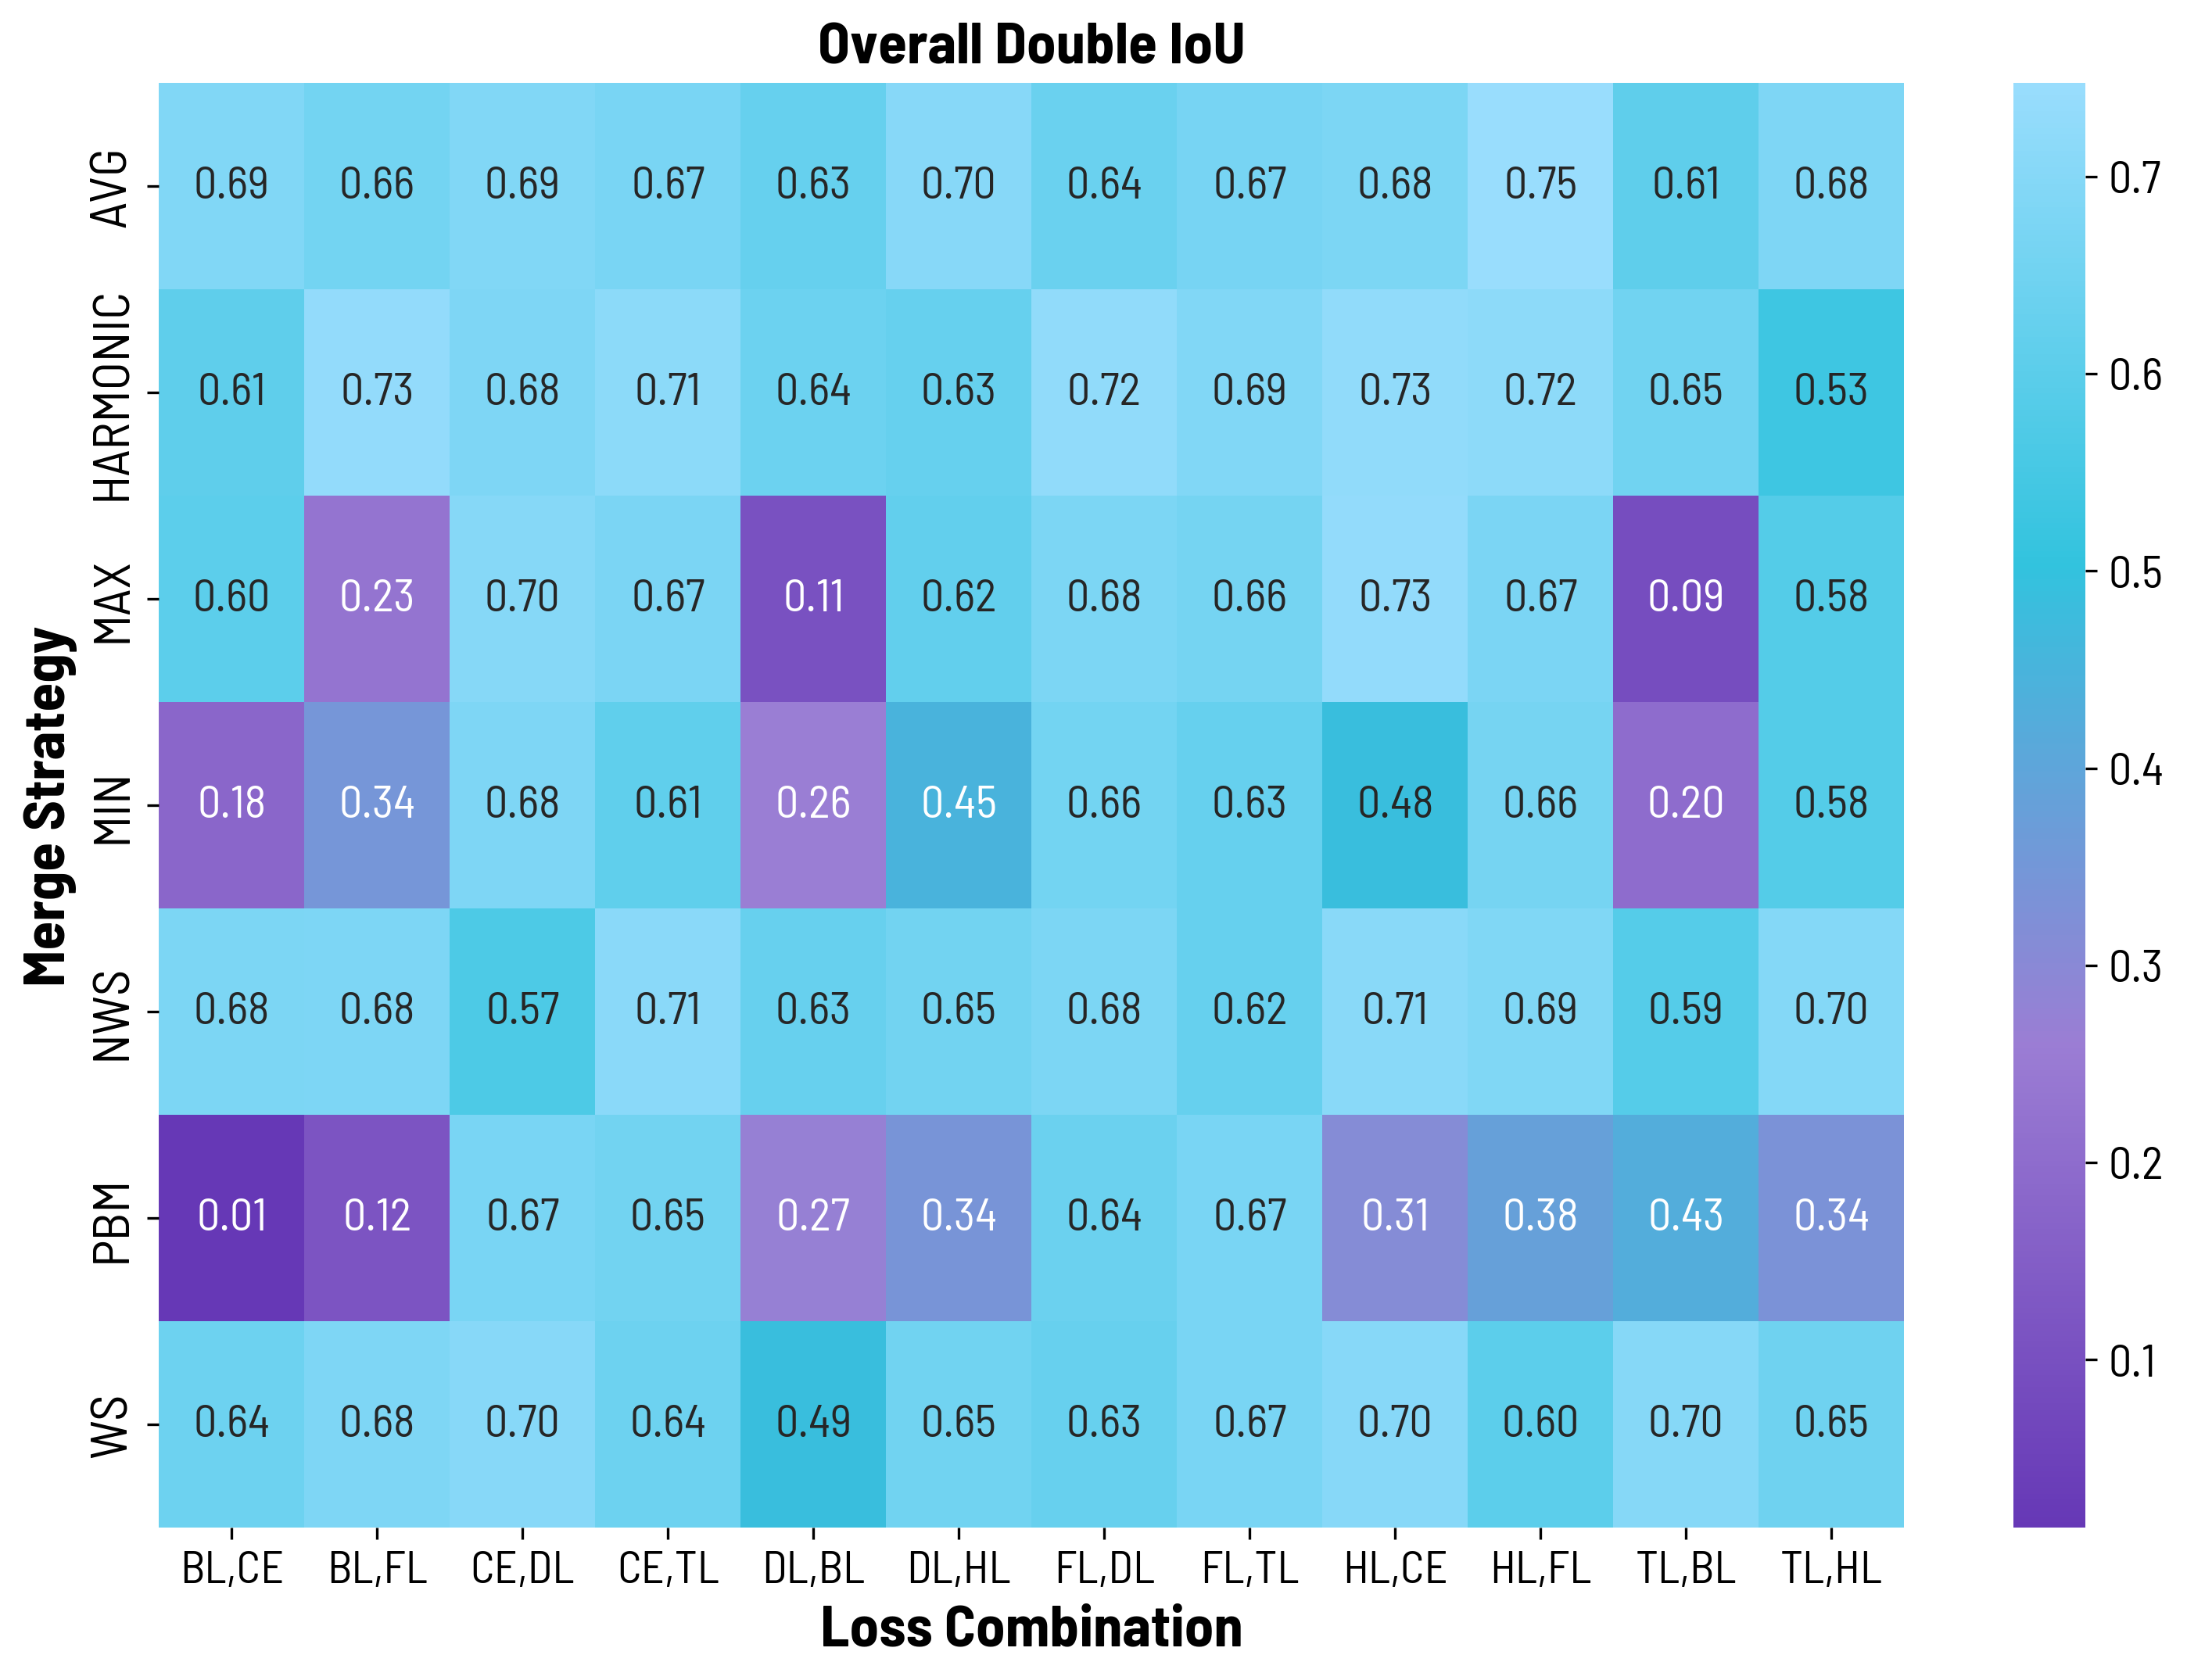
\includegraphics[width=\imgWidthcustom]{images/overall_results_double_medaka.png}}
  \subfigure[Overall performance of triple combinations]{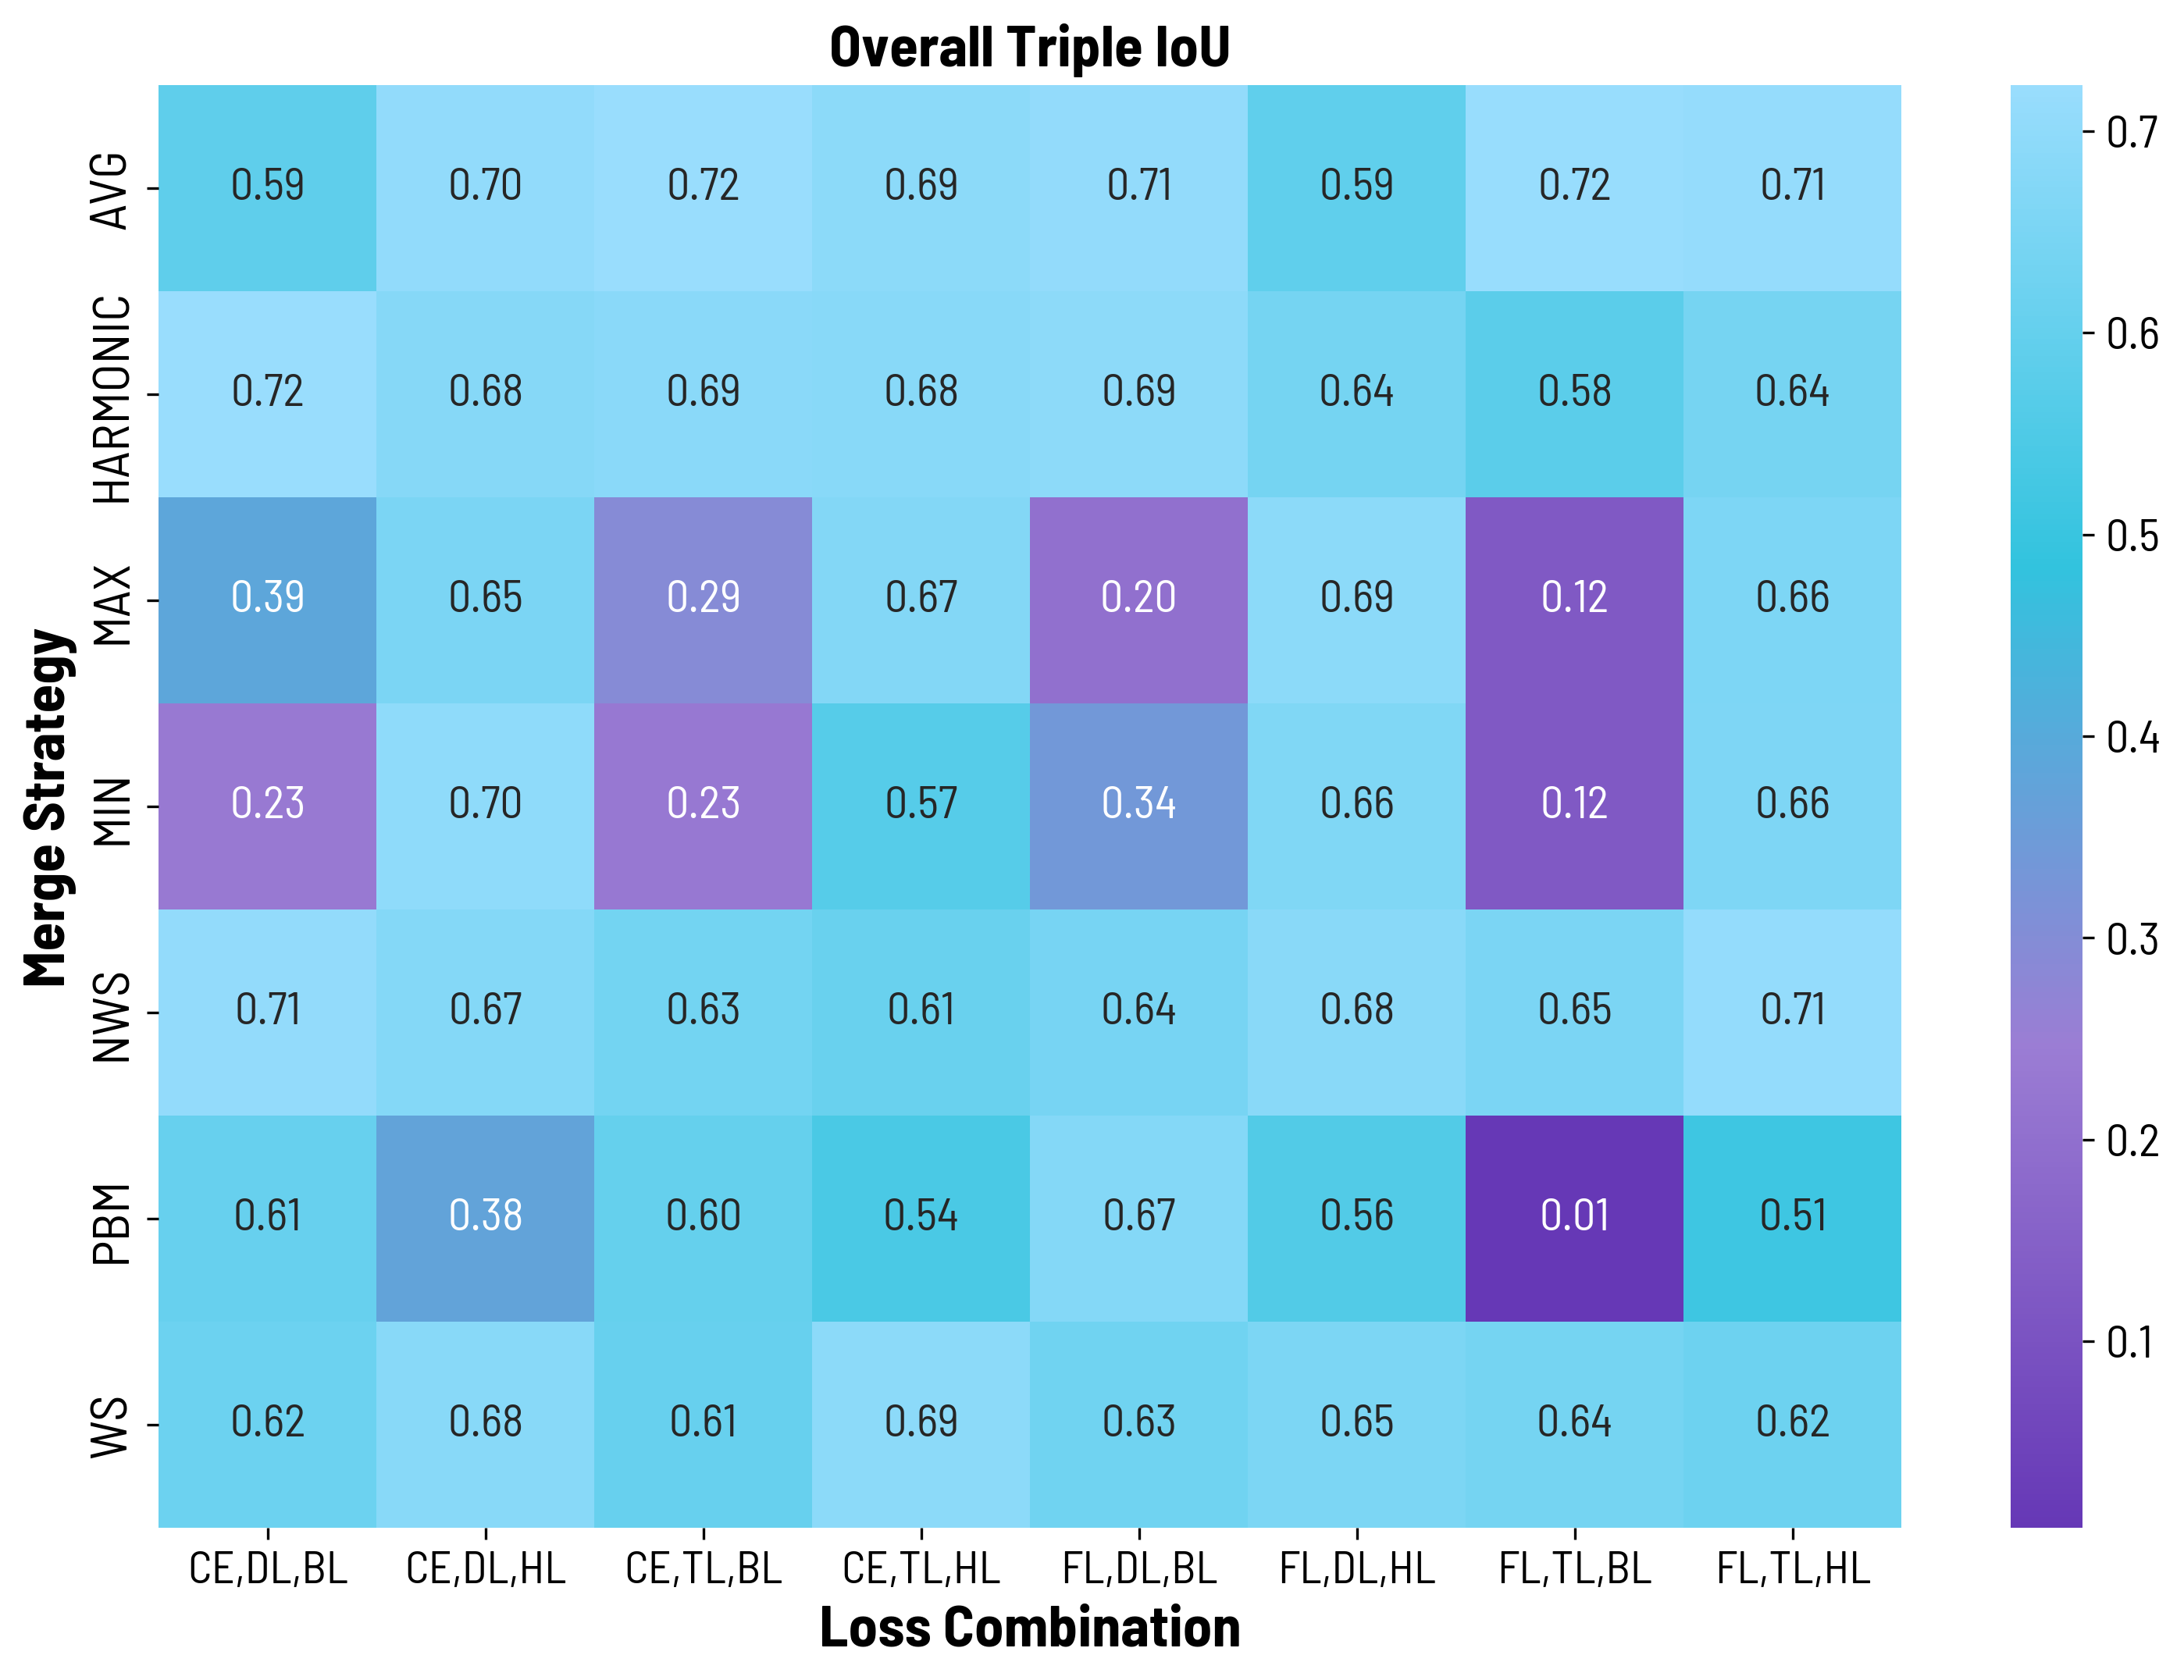
\includegraphics[width=\imgWidthcustom]{images/overall_results_triple_medaka.png}}
  \caption[Overall performance of triple combinations]{Average \ac{IoU} for all double and triple loss-merge combinations.}
  \label{overall_double_triple_medaka}
\end{figure}

These heatmaps, showcasing average scores, provide quick and intuitive insights into the framework's performance. For the double loss combinations, it is immediately apparent that the AVG, HARMONIC, NWS, and WS strategies excel, while the PBM, MIN, and MAX strategies underperform. Columns demonstrating the averages for each loss combination enable rapid identification of high-performing options. The same advantages hold for the heatmap depicting the triple loss combinations.

Although a direct comparison between the double and triple loss combinations is not feasible, a noteworthy characteristic observed in both categories is the similar performance trend across different merge strategies. Specifically, the MIN and MAX strategies consistently demonstrated suboptimal performance for both loss combinations. On the other hand, the PBM strategy has performed better on average for triple loss combinations.
%----------------------------------DISCRETE PERFORMANCE (Medaka)-------------------------%
\subsubsection*{Discrete Performance}
The discrete performance results illustrate additional graphs from the loss combination and merge strategy perspective. The bars of each graph are displayed in descending order from left to right by \ac{IoU}. The discrete performance results display models from configuration no. 2, which consists of 360 models.

\textbf{Loss combination results}\newline
\figref{loss_combination_results_medaka_short} displays all average double and triple loss combination results in descending order. We can see that the top six double loss combinations show similar performance and even topping the top-performing baseline results. Interestingly all losses, including the \ac{BL}, are performing rather low for the double and triple loss combinations.

Looking at table \ref{tab:loss_combination_results_medaka_double_long}, which displays the averages of the top three performing models for each double loss combination and selection percentage, there are three combinations HL, FL, CE, DL, and HL, CE which exceed the top three baseline averages. 
\begin{figure}[H]%[htbp]
  \centering
  \subfigure[Average IoU for Each Double Loss Combination]{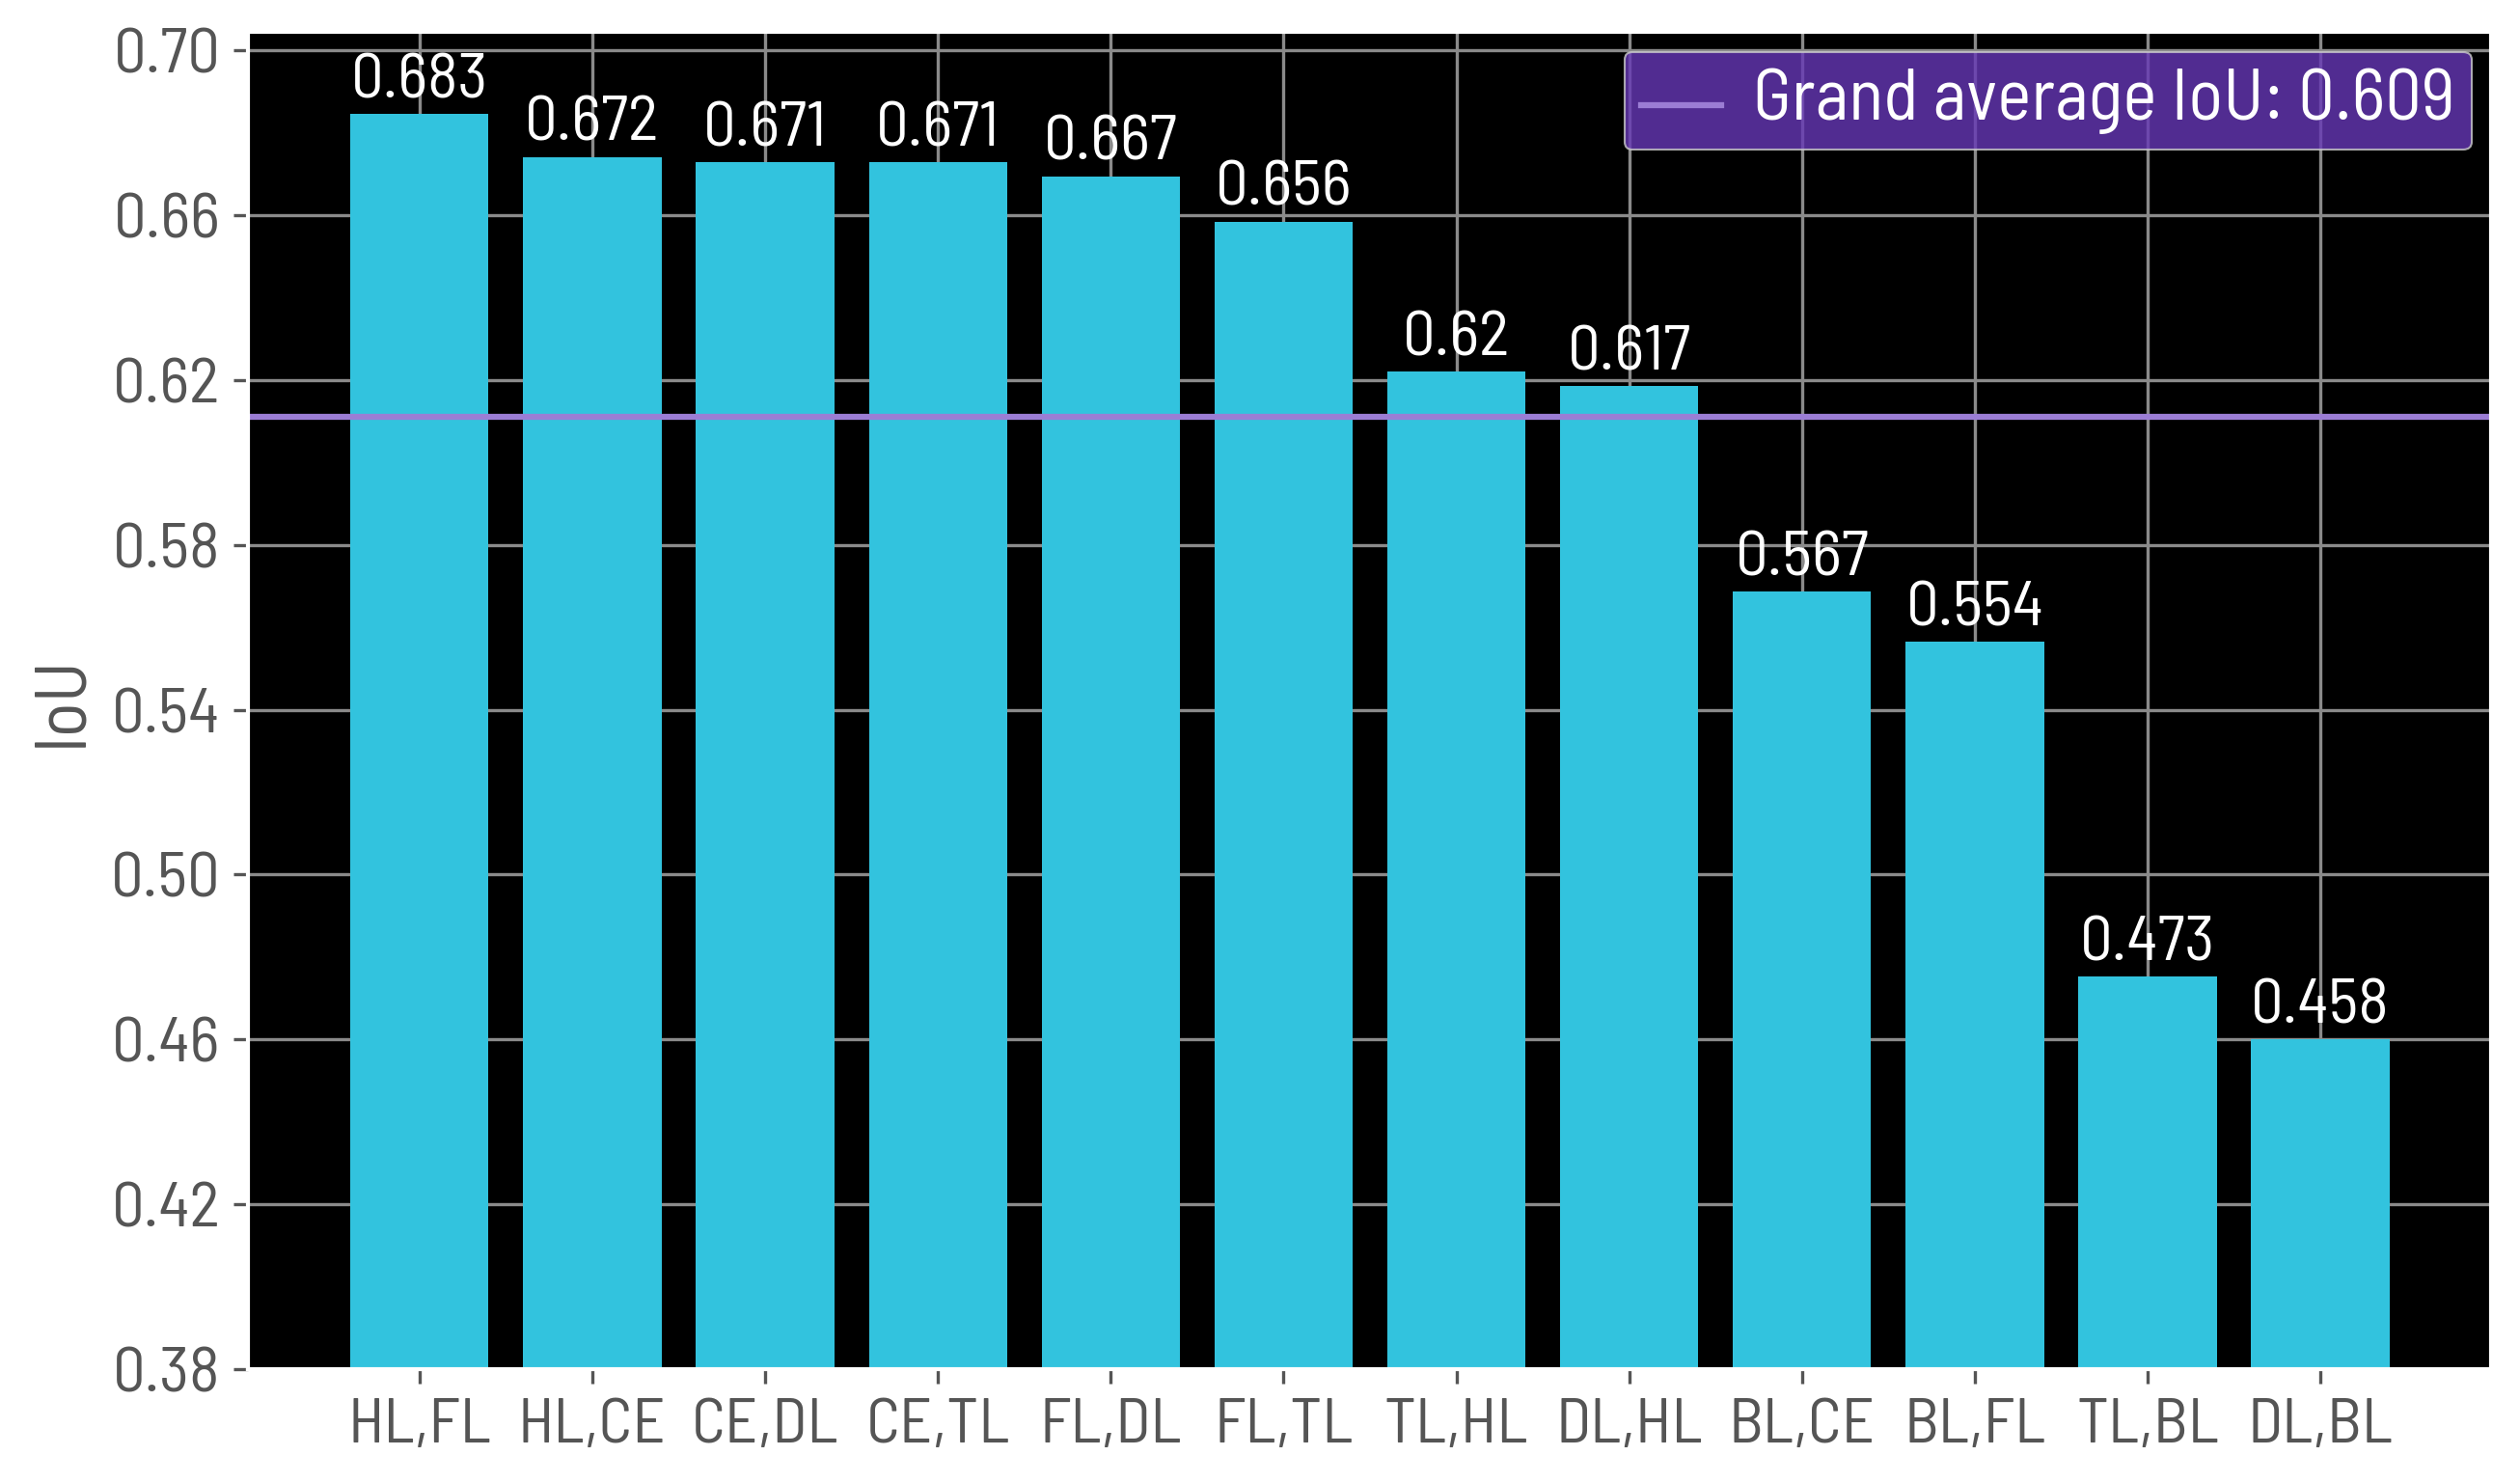
\includegraphics[width=\imgWidthcustom]{images/loss_combination_results_medaka_double_short_total.png}}
  \subfigure[Average IoU for Each Triple Loss Combination]{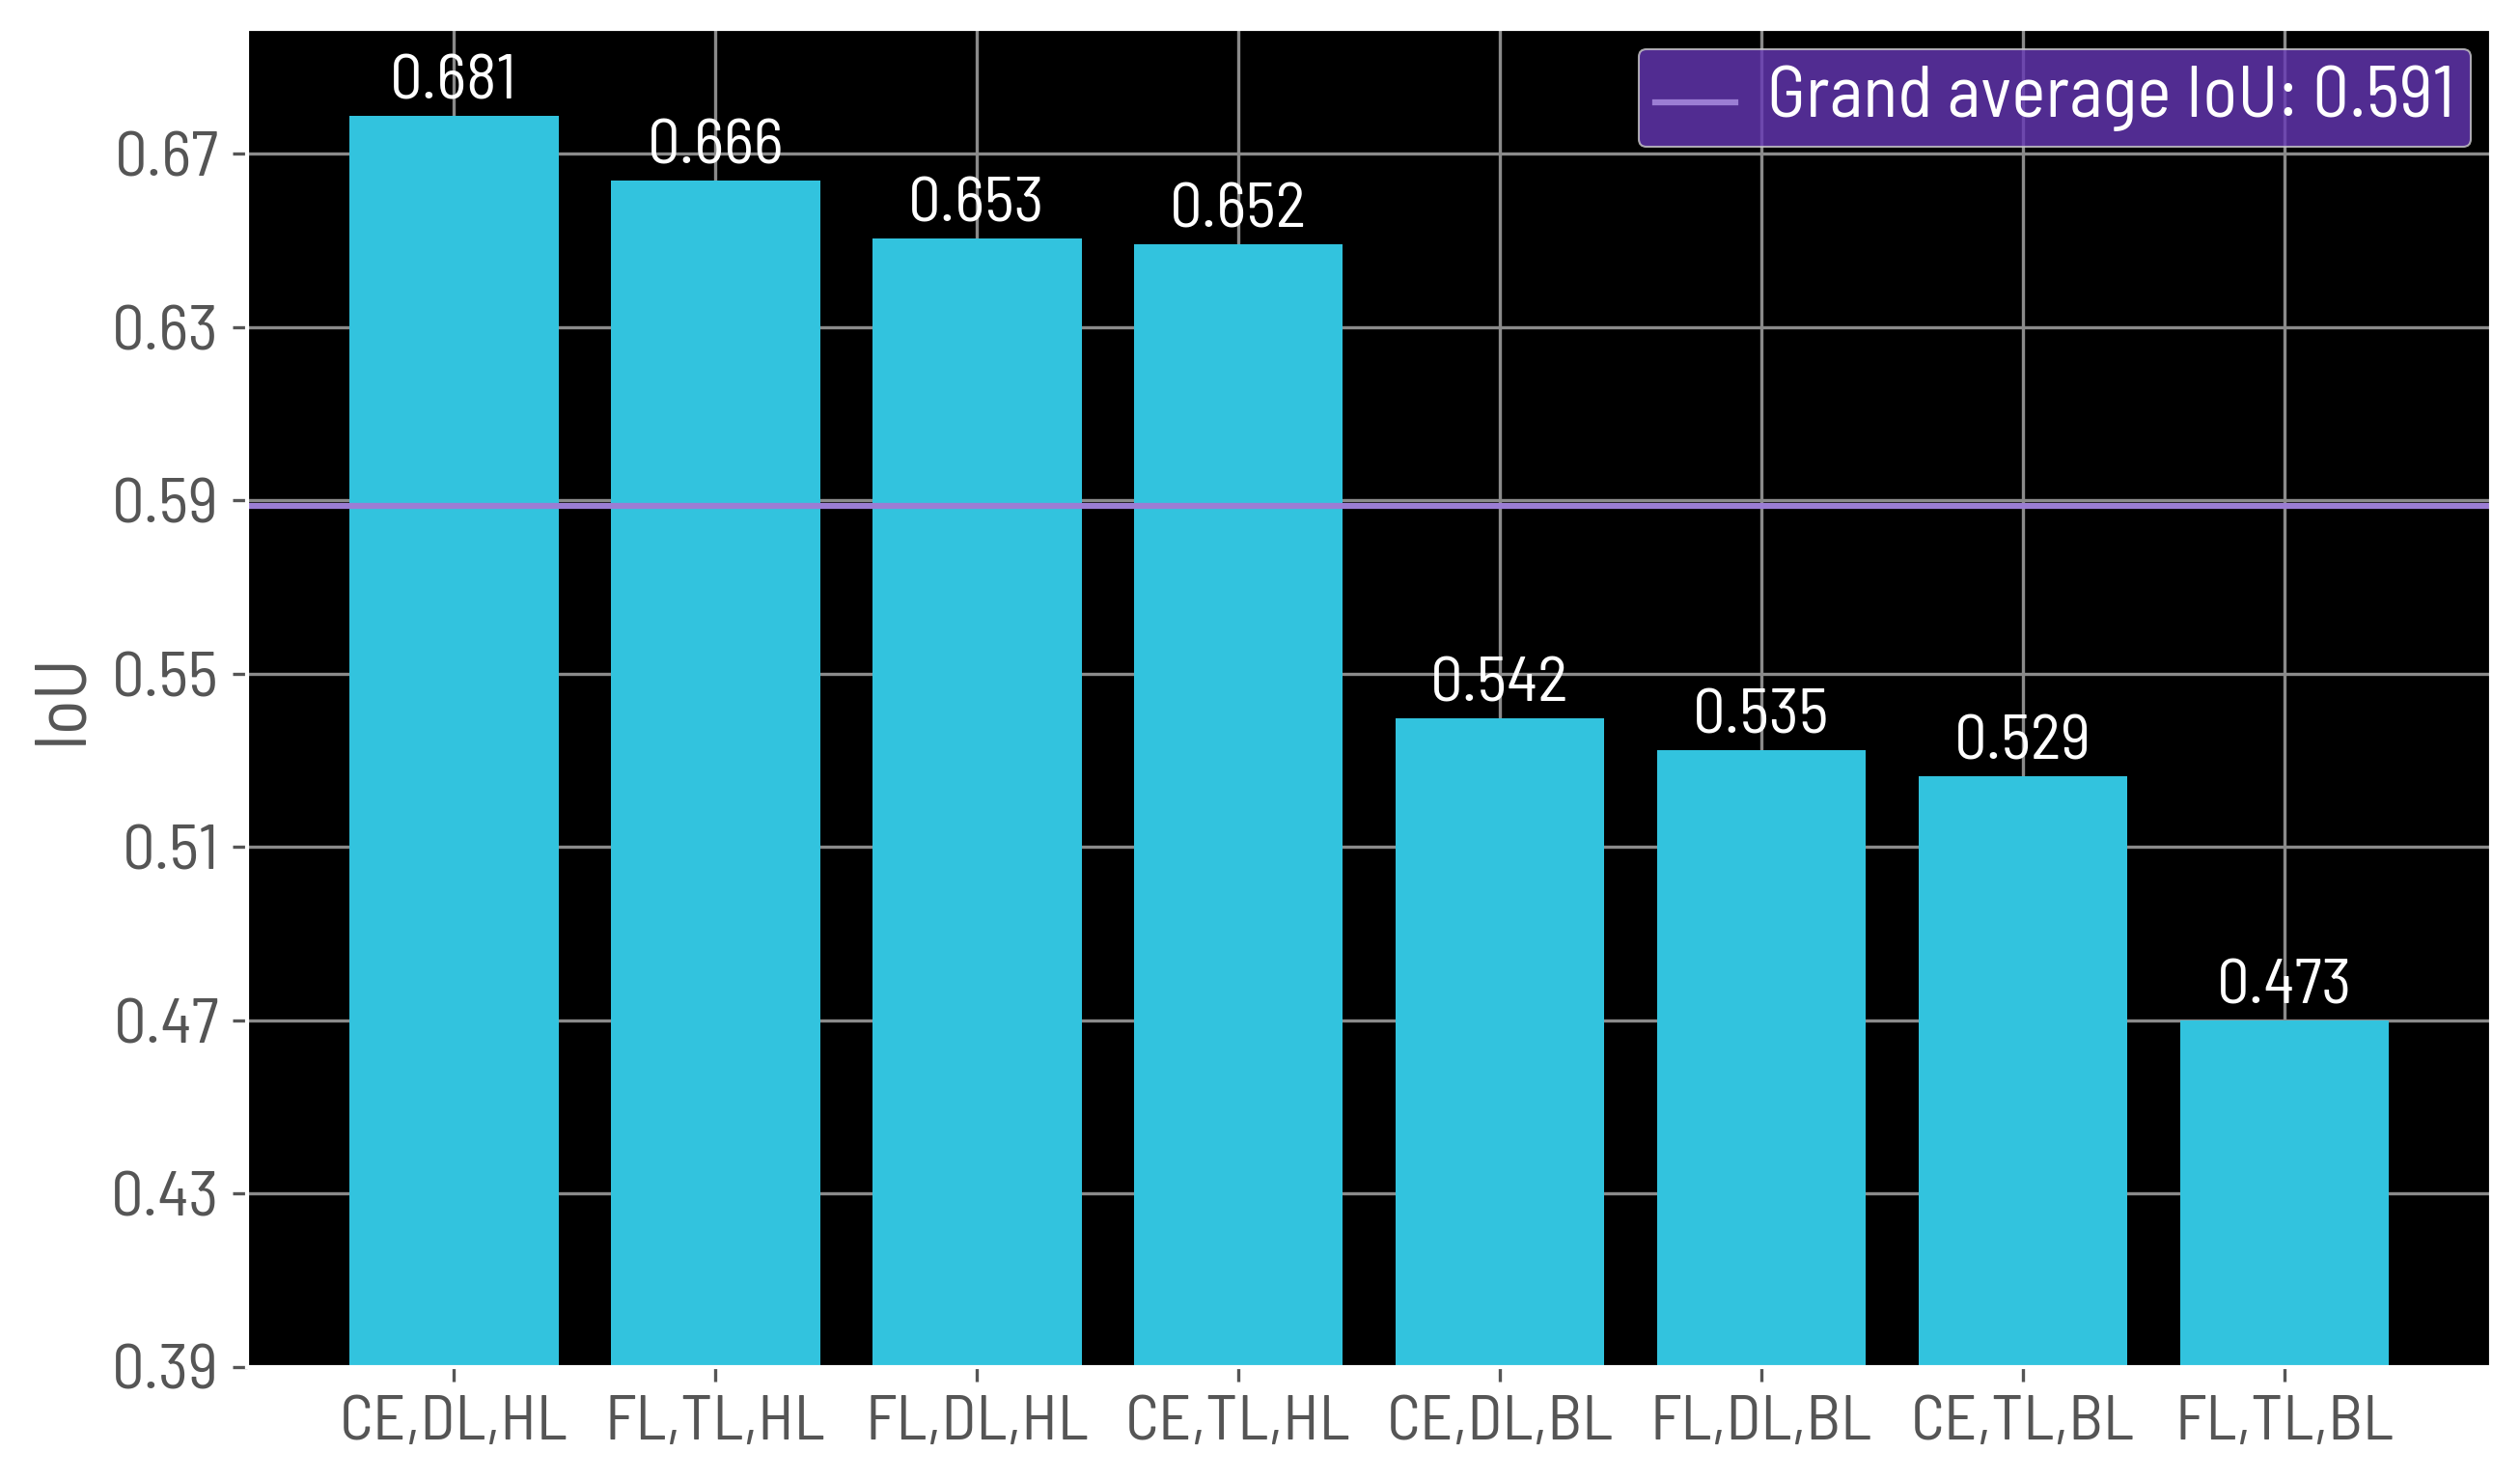
\includegraphics[width=\imgWidthcustom]{images/loss_combination_results_medaka_triple_short_total.png}}
  \caption[Average IoU for Loss Combination (Medaka)]{The figures showcase the average \ac{IoU} for loss combination, as well as their corresponding selection percentages, derived from an extensive set of 360 models trained on the \ac{MFD}.}
  \label{loss_combination_results_medaka_short}
\end{figure}

\textbf{Merge strategy results}\newline
\figref{merge_strategy_results_medaka_short} illustrates the average scores for all trained models by merge strategy. Both graphs indicate a rather stable performance except for the MAX and MIN strategies.
\begin{figure}[H]%[htbp]
  \centering
  \subfigure[Average IoU for Each Double Merge Strategy]{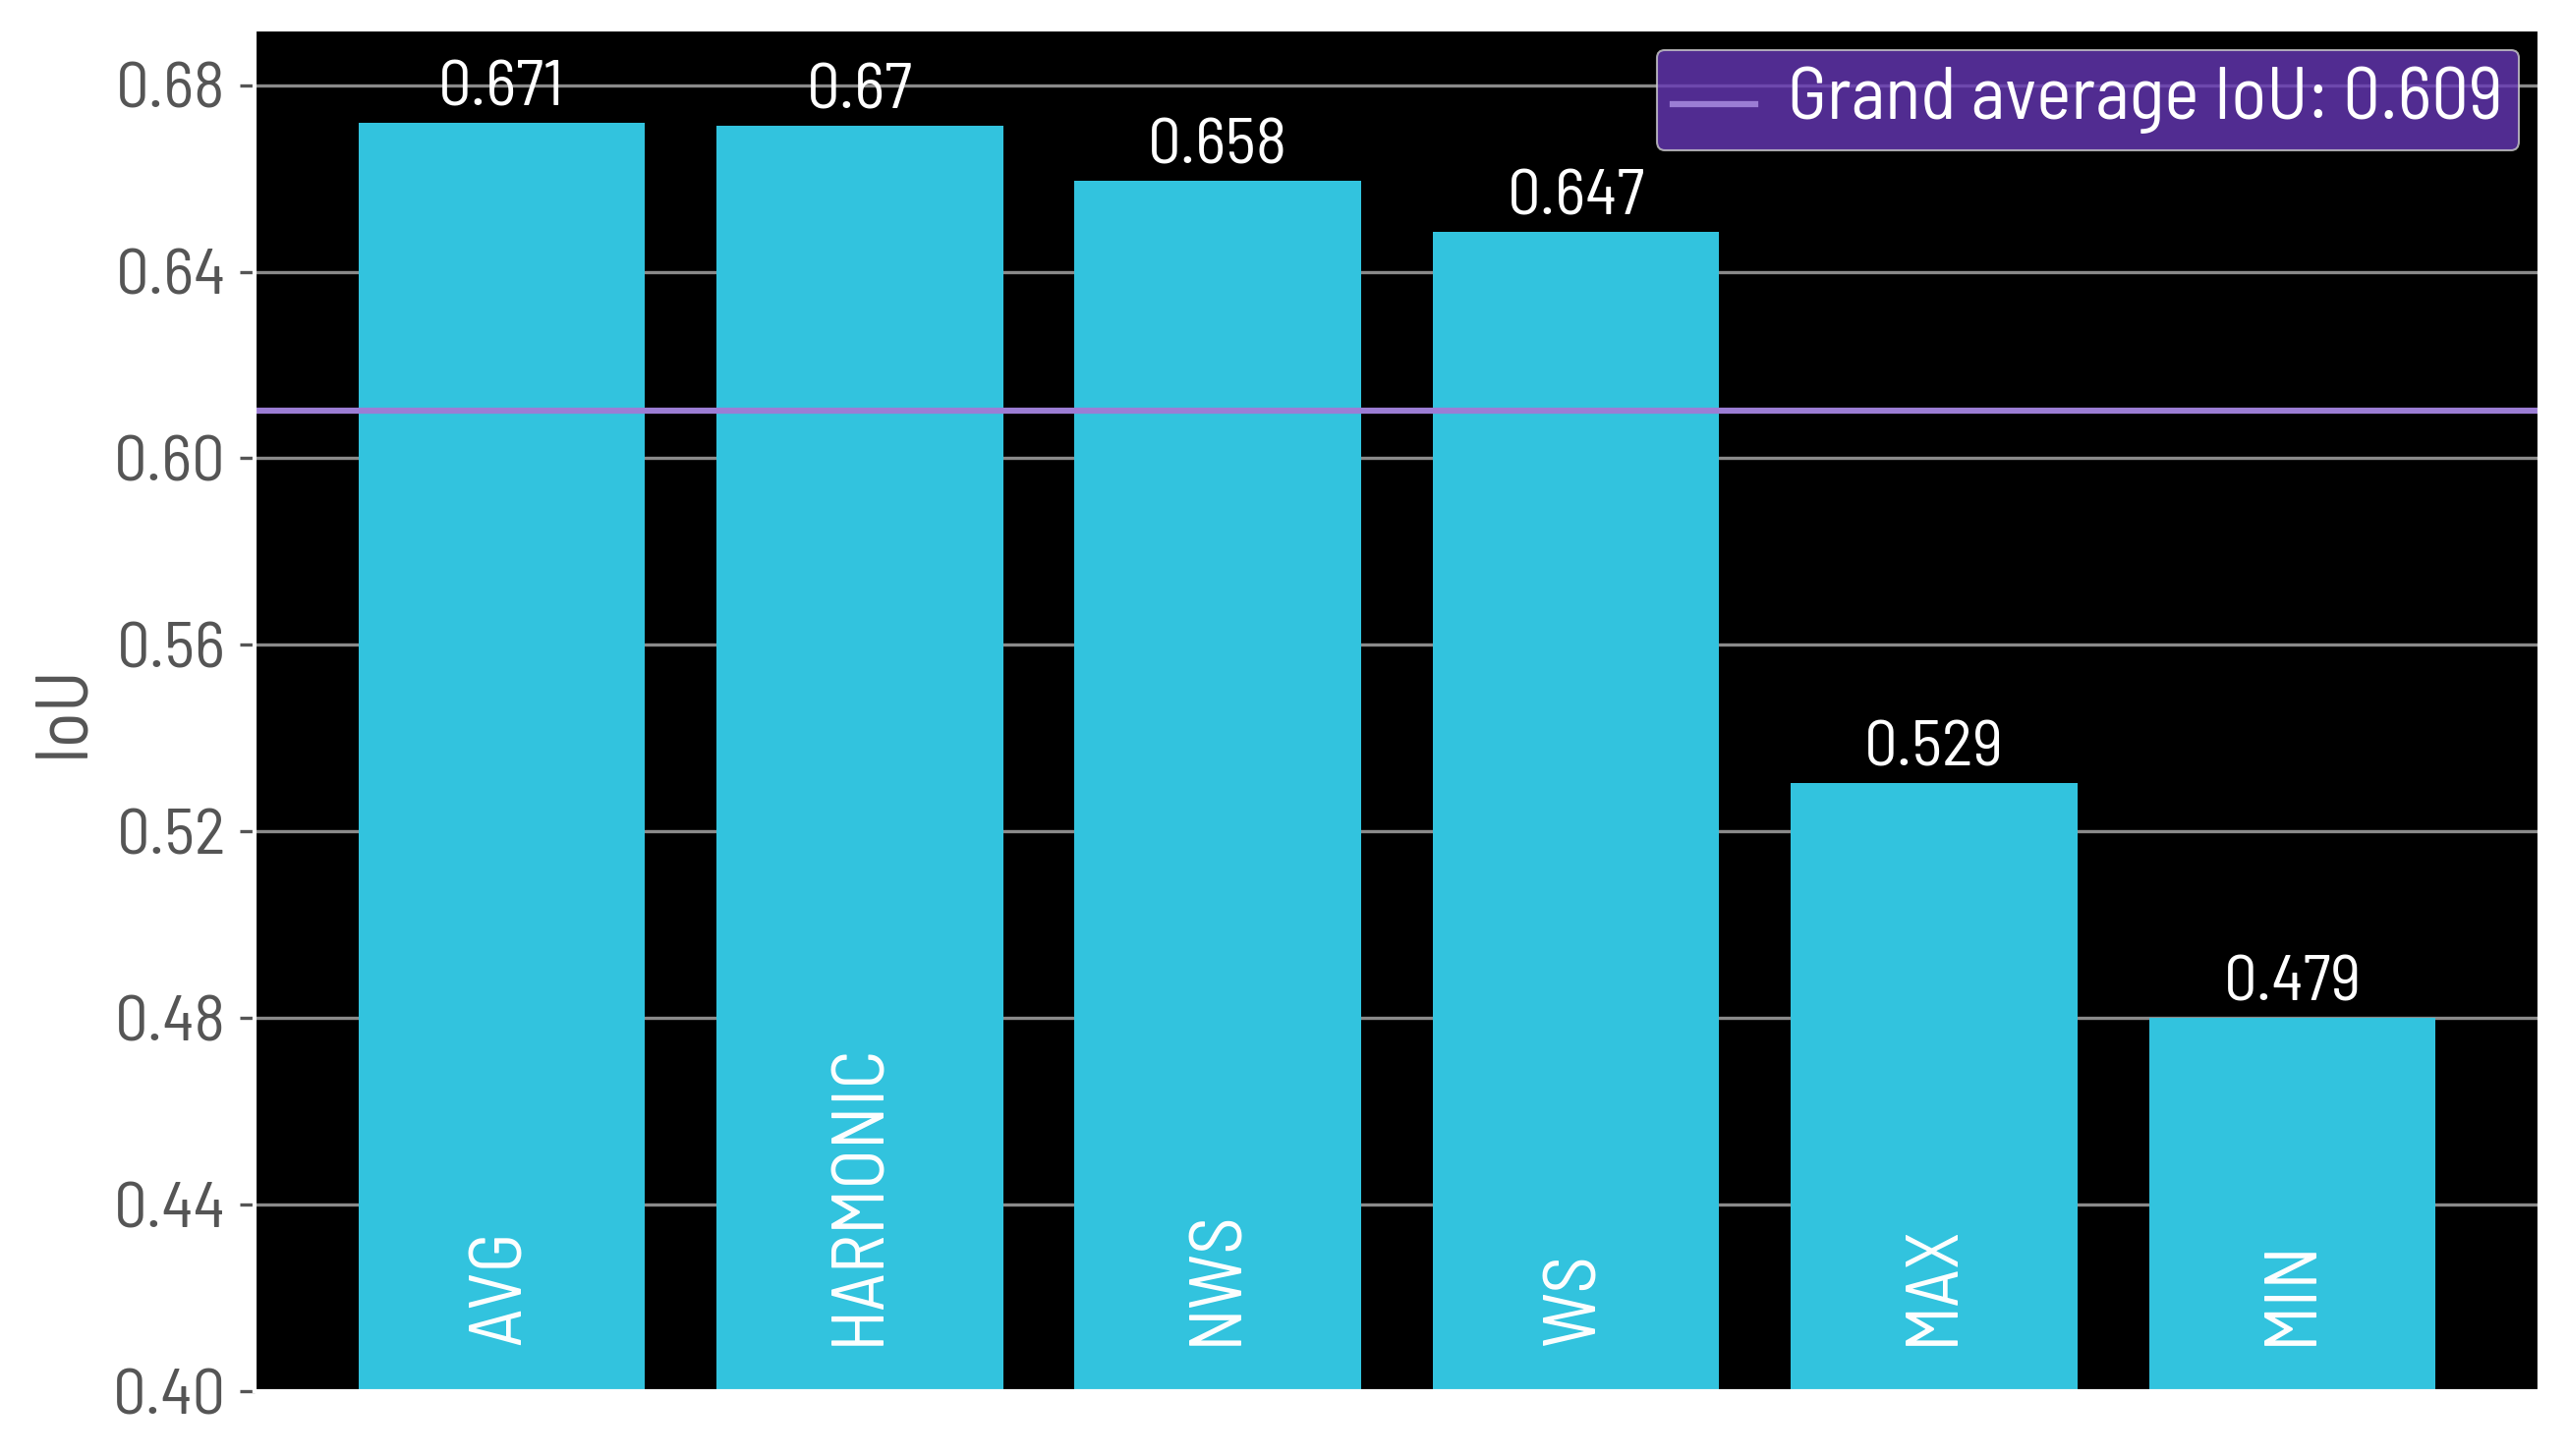
\includegraphics[width=\imgWidthcustom]{images/merge_strategy_results_medaka_double_short_total.png}}
  \subfigure[Average IoU for Each Triple Merge Strategy]{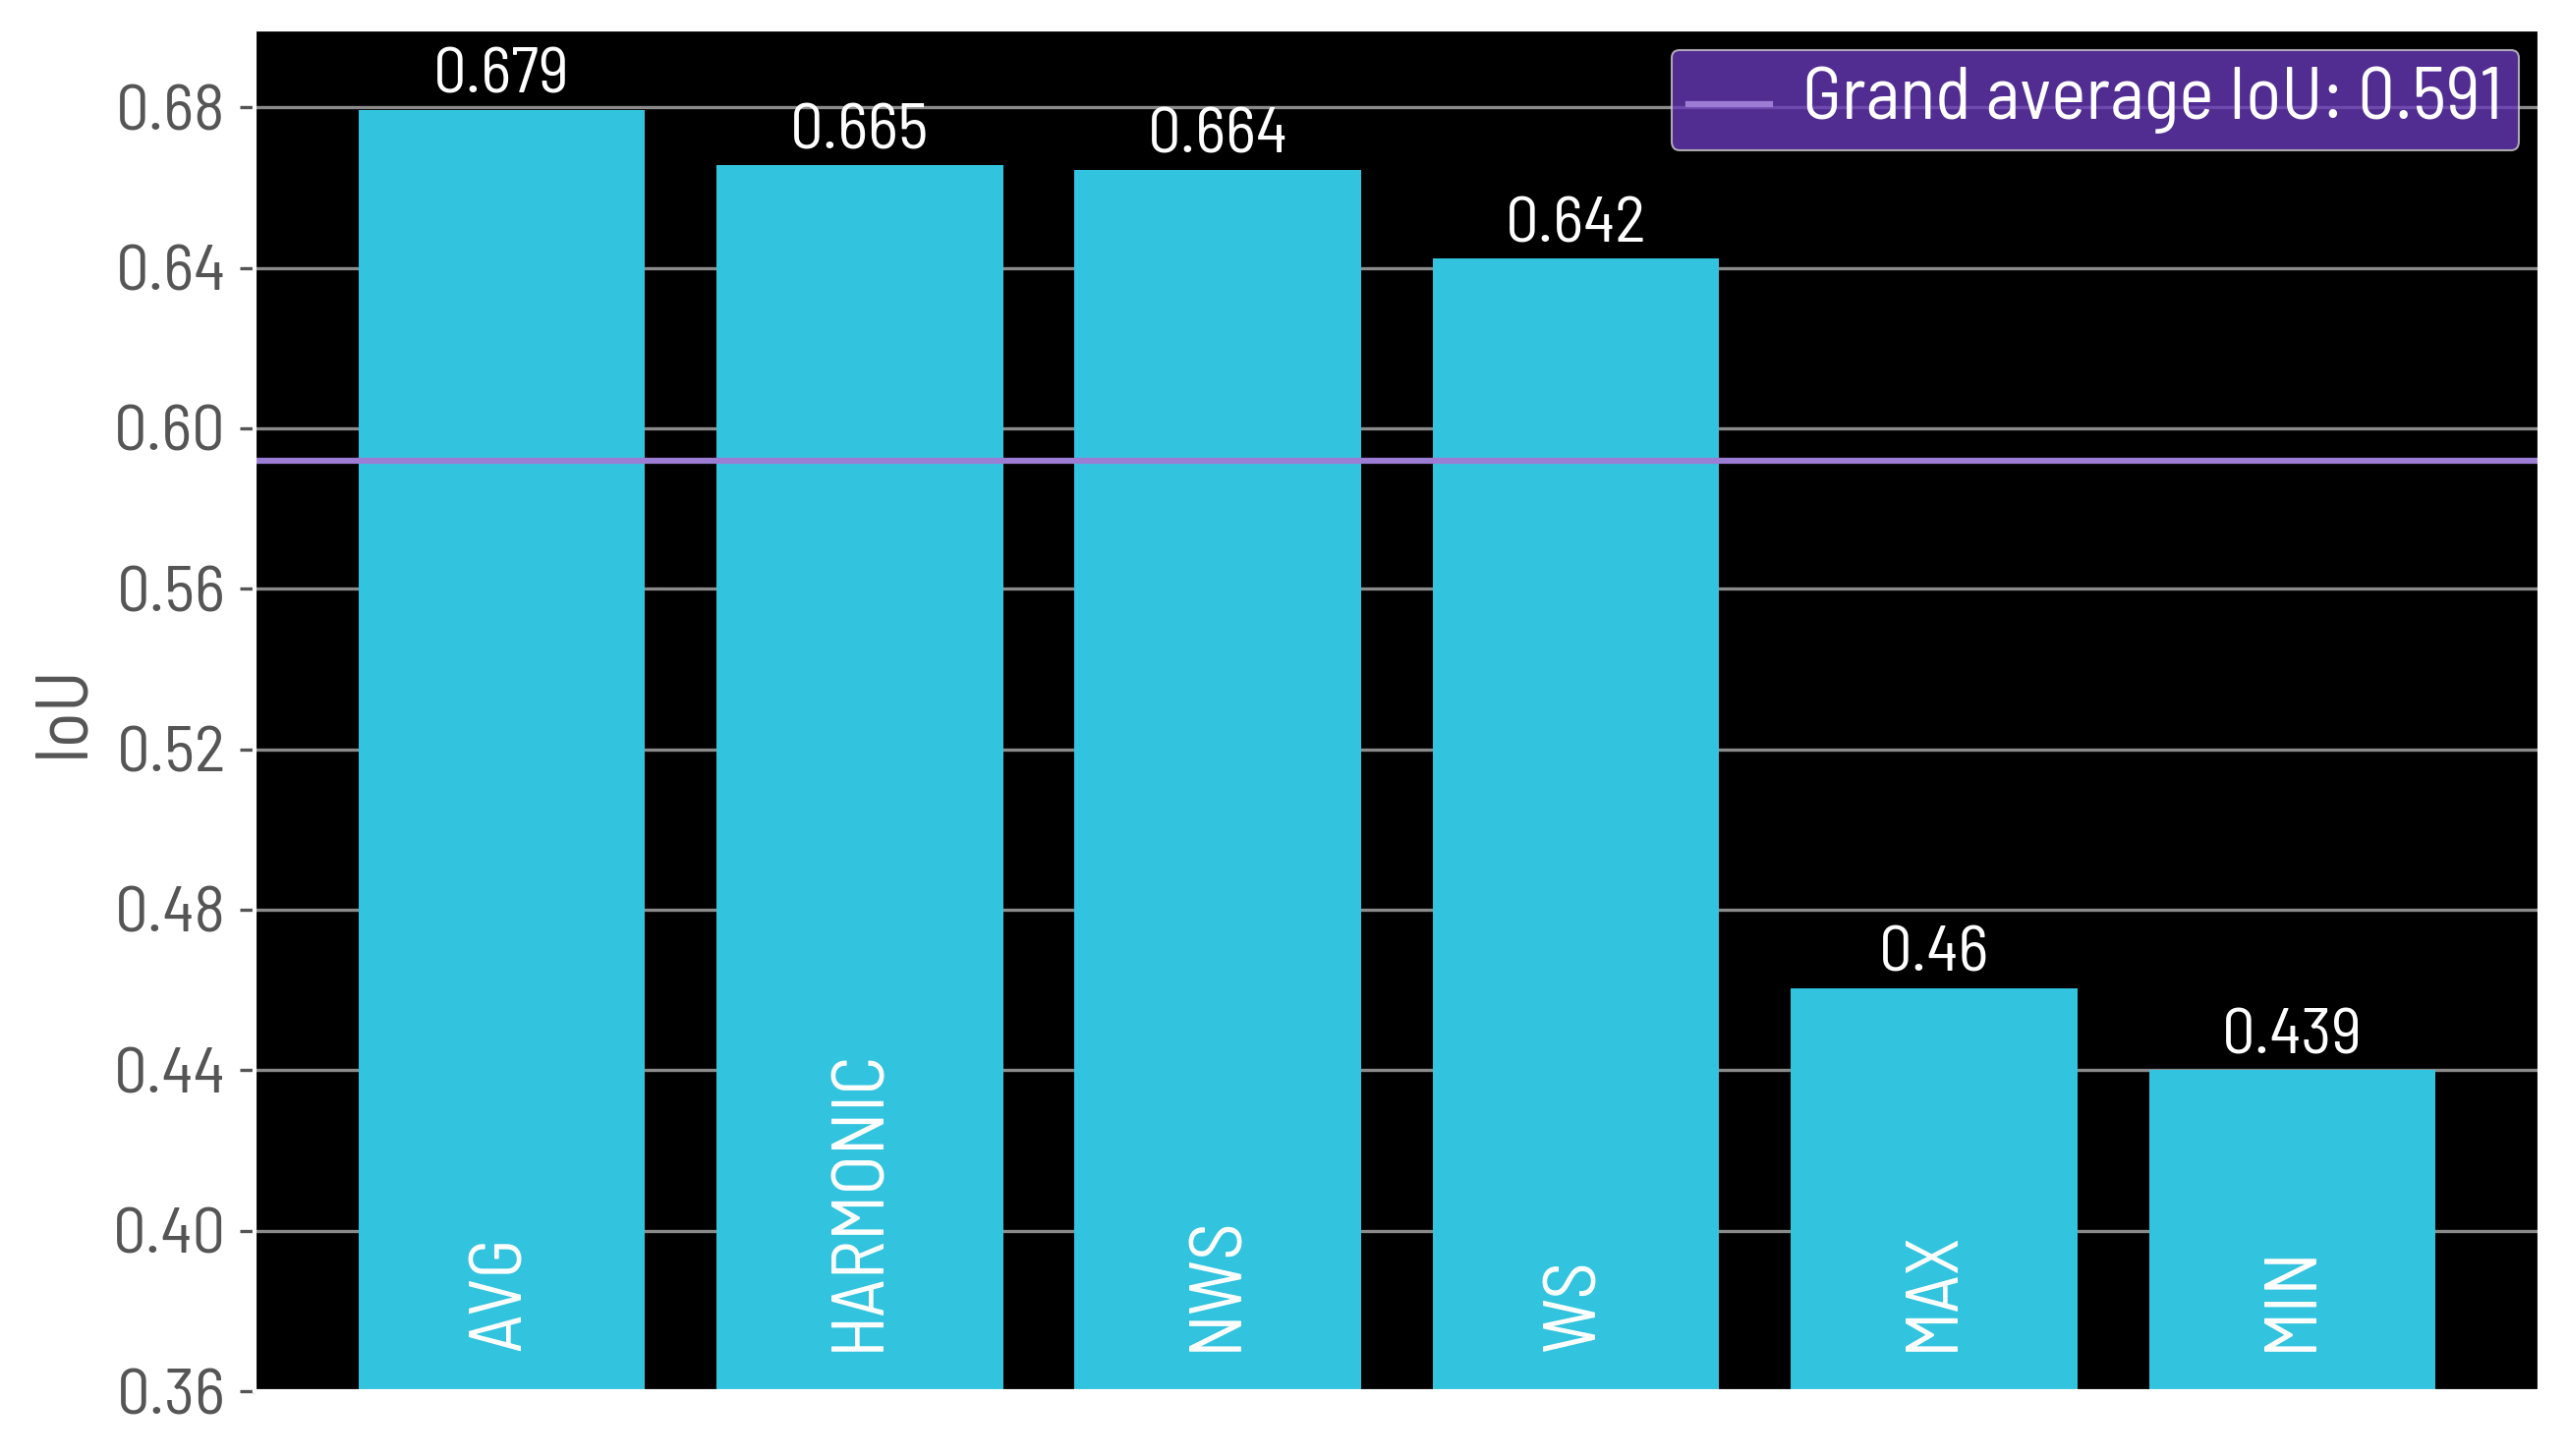
\includegraphics[width=\imgWidthcustom]{images/merge_strategy_results_medaka_triple_short_total.png}}
  \caption[Average IoU for Each Merge Strategy (Medaka)]{The figures showcase the average \ac{IoU} for each merge strategy, as well as their corresponding selection percentages, derived from an extensive set of 360 models trained on the \ac{MFD}.}
  \label{merge_strategy_results_medaka_short}
\end{figure}

%----------------------------------CONTINOUS PERFORMANCE (Medaka)------------------------%
\subsubsection*{Continuous Performance}
The models examined in this section were trained to utilize configuration no. 3 as outlined in table \ref{tab:final_configuration_list}. Generally, comparing models across different configurations may present challenges due to differing numbers. While the model count in discrete configurations is predefined, continuous configurations employ a Hyperband search algorithm to identify suitable hyperparameters for the performance-based merge strategy. \figref{continous_loss_combination_results_medaka_short} presents the average result for each loss combination implementing this strategy. The bars also depict the model count, which can vary significantly due to the Hyperband algorithm's specific selection mechanism. Notably, top-performing combinations were chosen more frequently, particularly in the case of high-performing double-loss combinations.

Interestingly, while some double loss combinations with the HL performed commendably in discrete configurations, combinations involving boundary-based elements demonstrated poor performance when using the performance-based strategy for double losses. Conversely, at least among the top performers, the BL combinations surpassed the HL combinations for triple losses.
\begin{figure}[H]%[htbp]
  \centering
  \subfigure[Average IoU for Each Double Loss Combination]{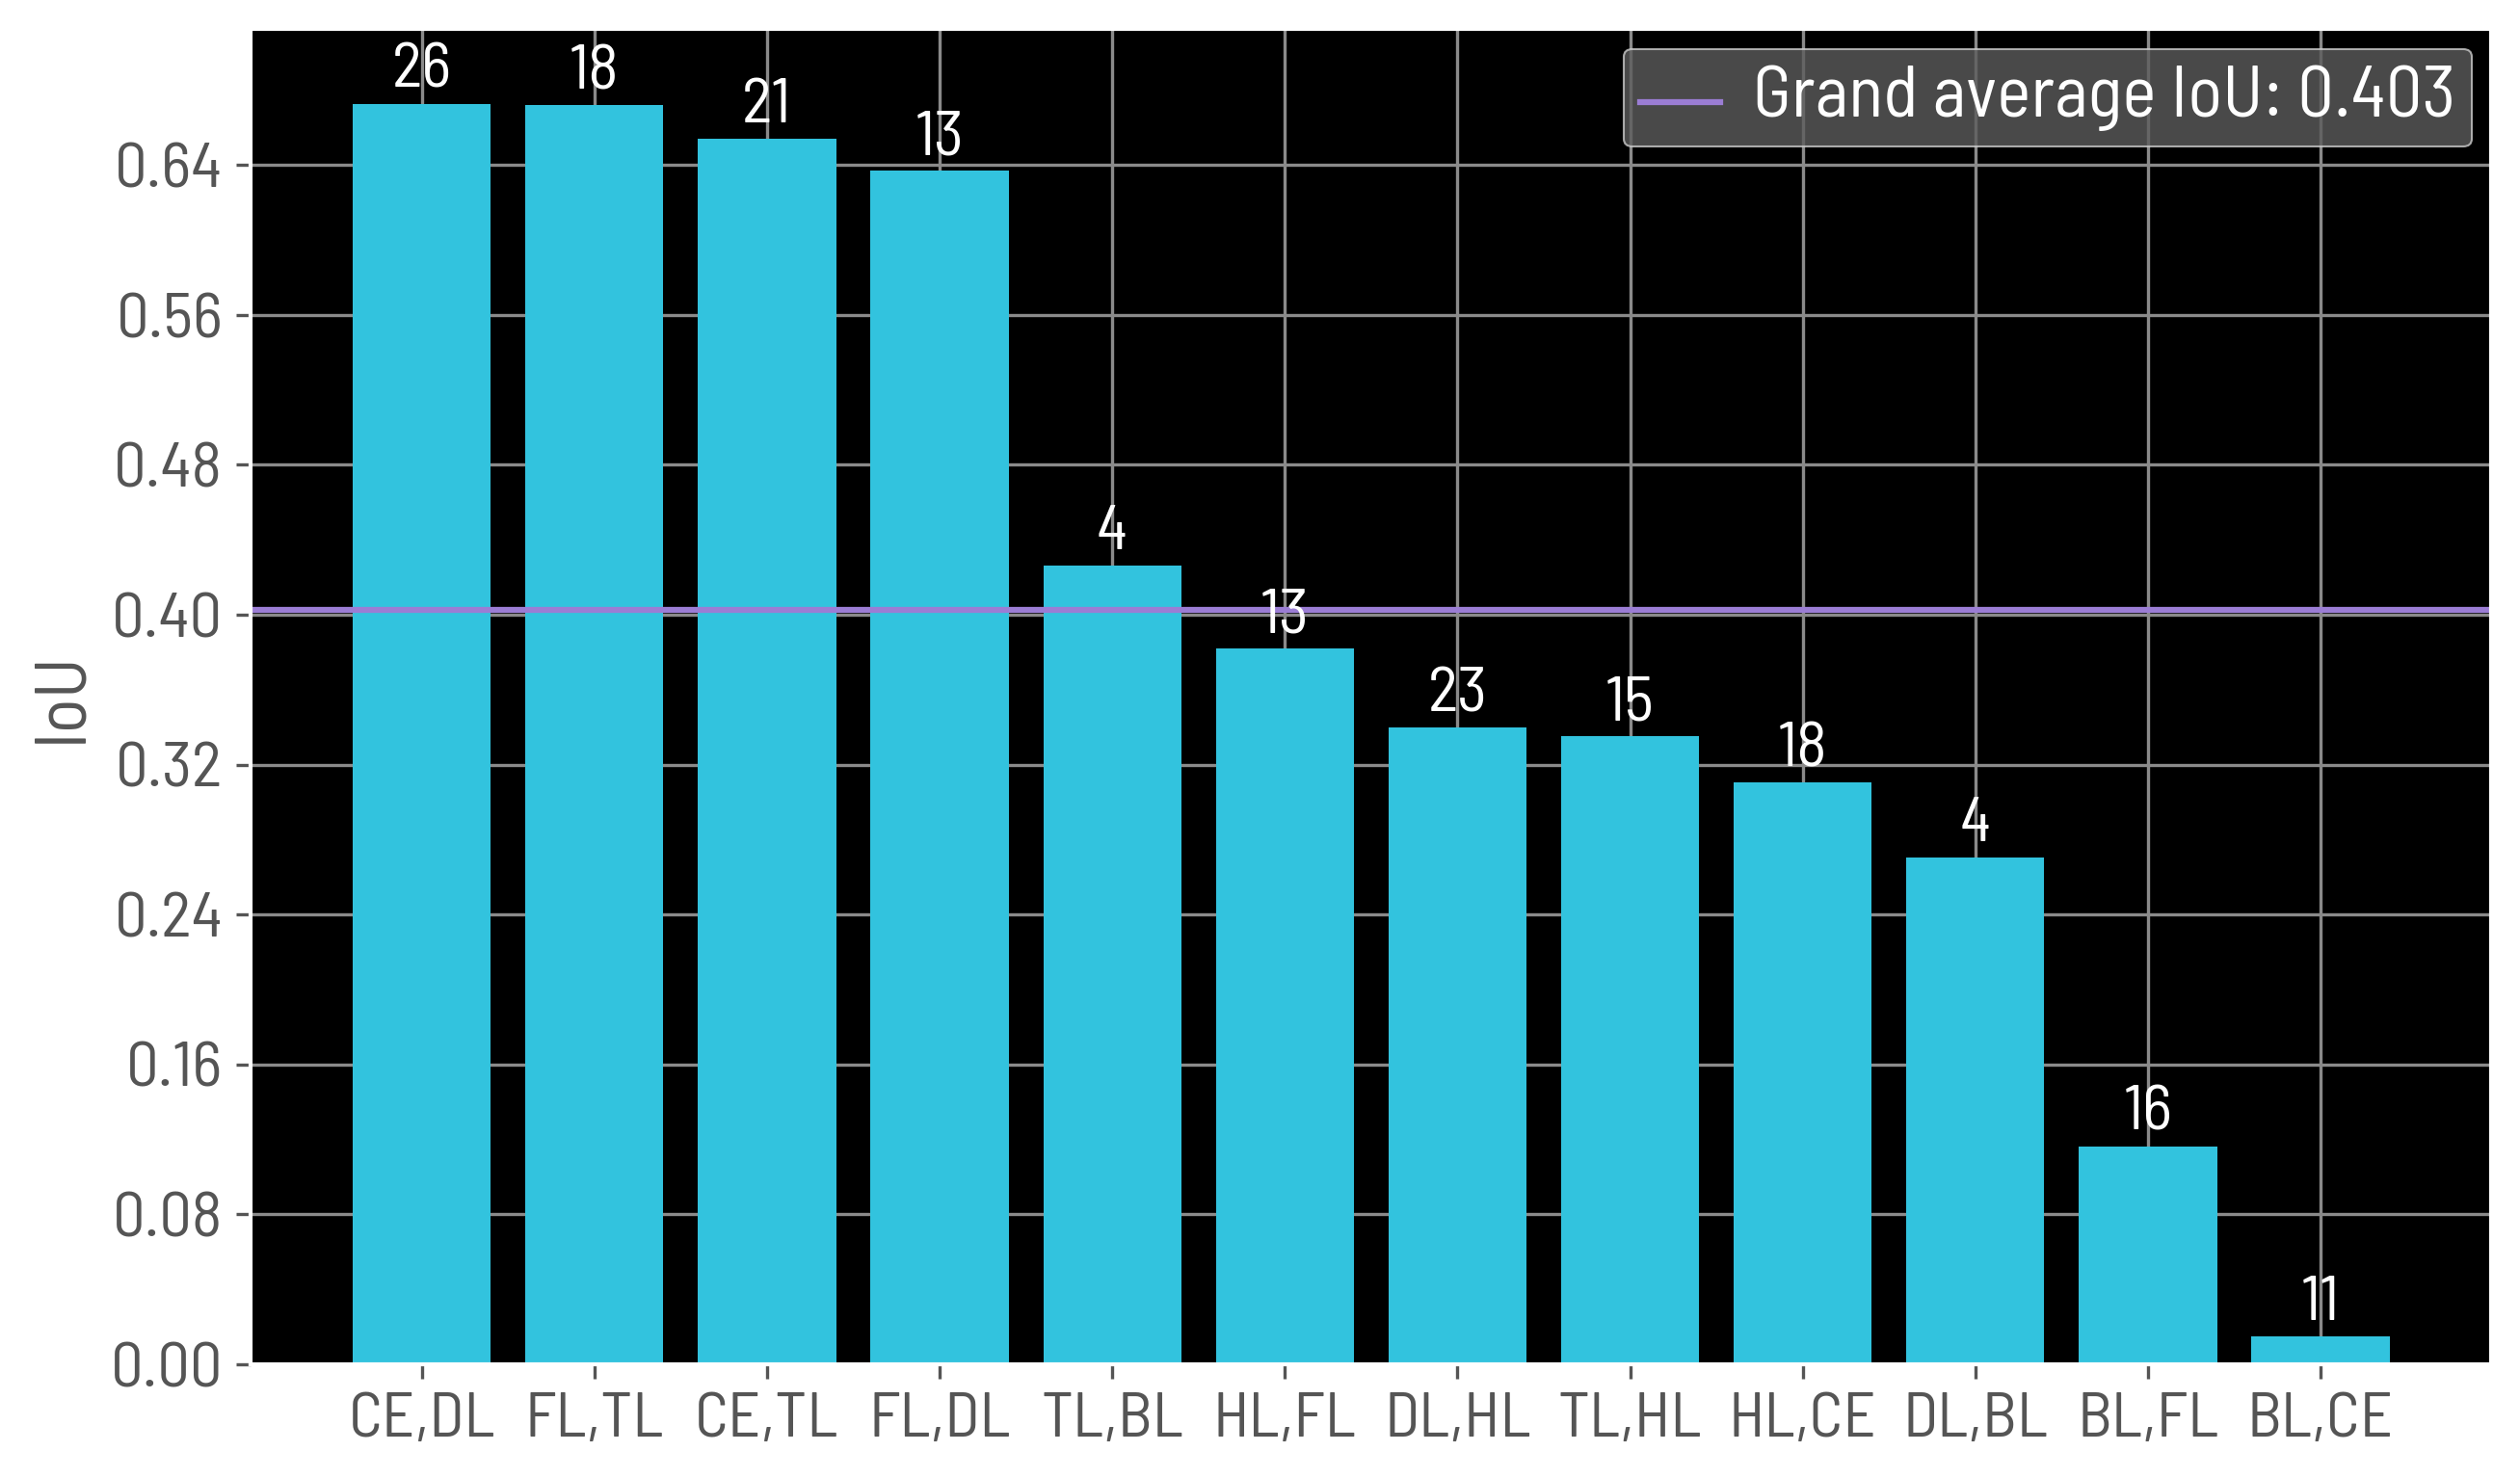
\includegraphics[width=\imgWidthcustom]{images/continous_loss_combination_results_medaka_double_short_total.png}}
  \subfigure[Average IoU for Each Triple Loss Combination]{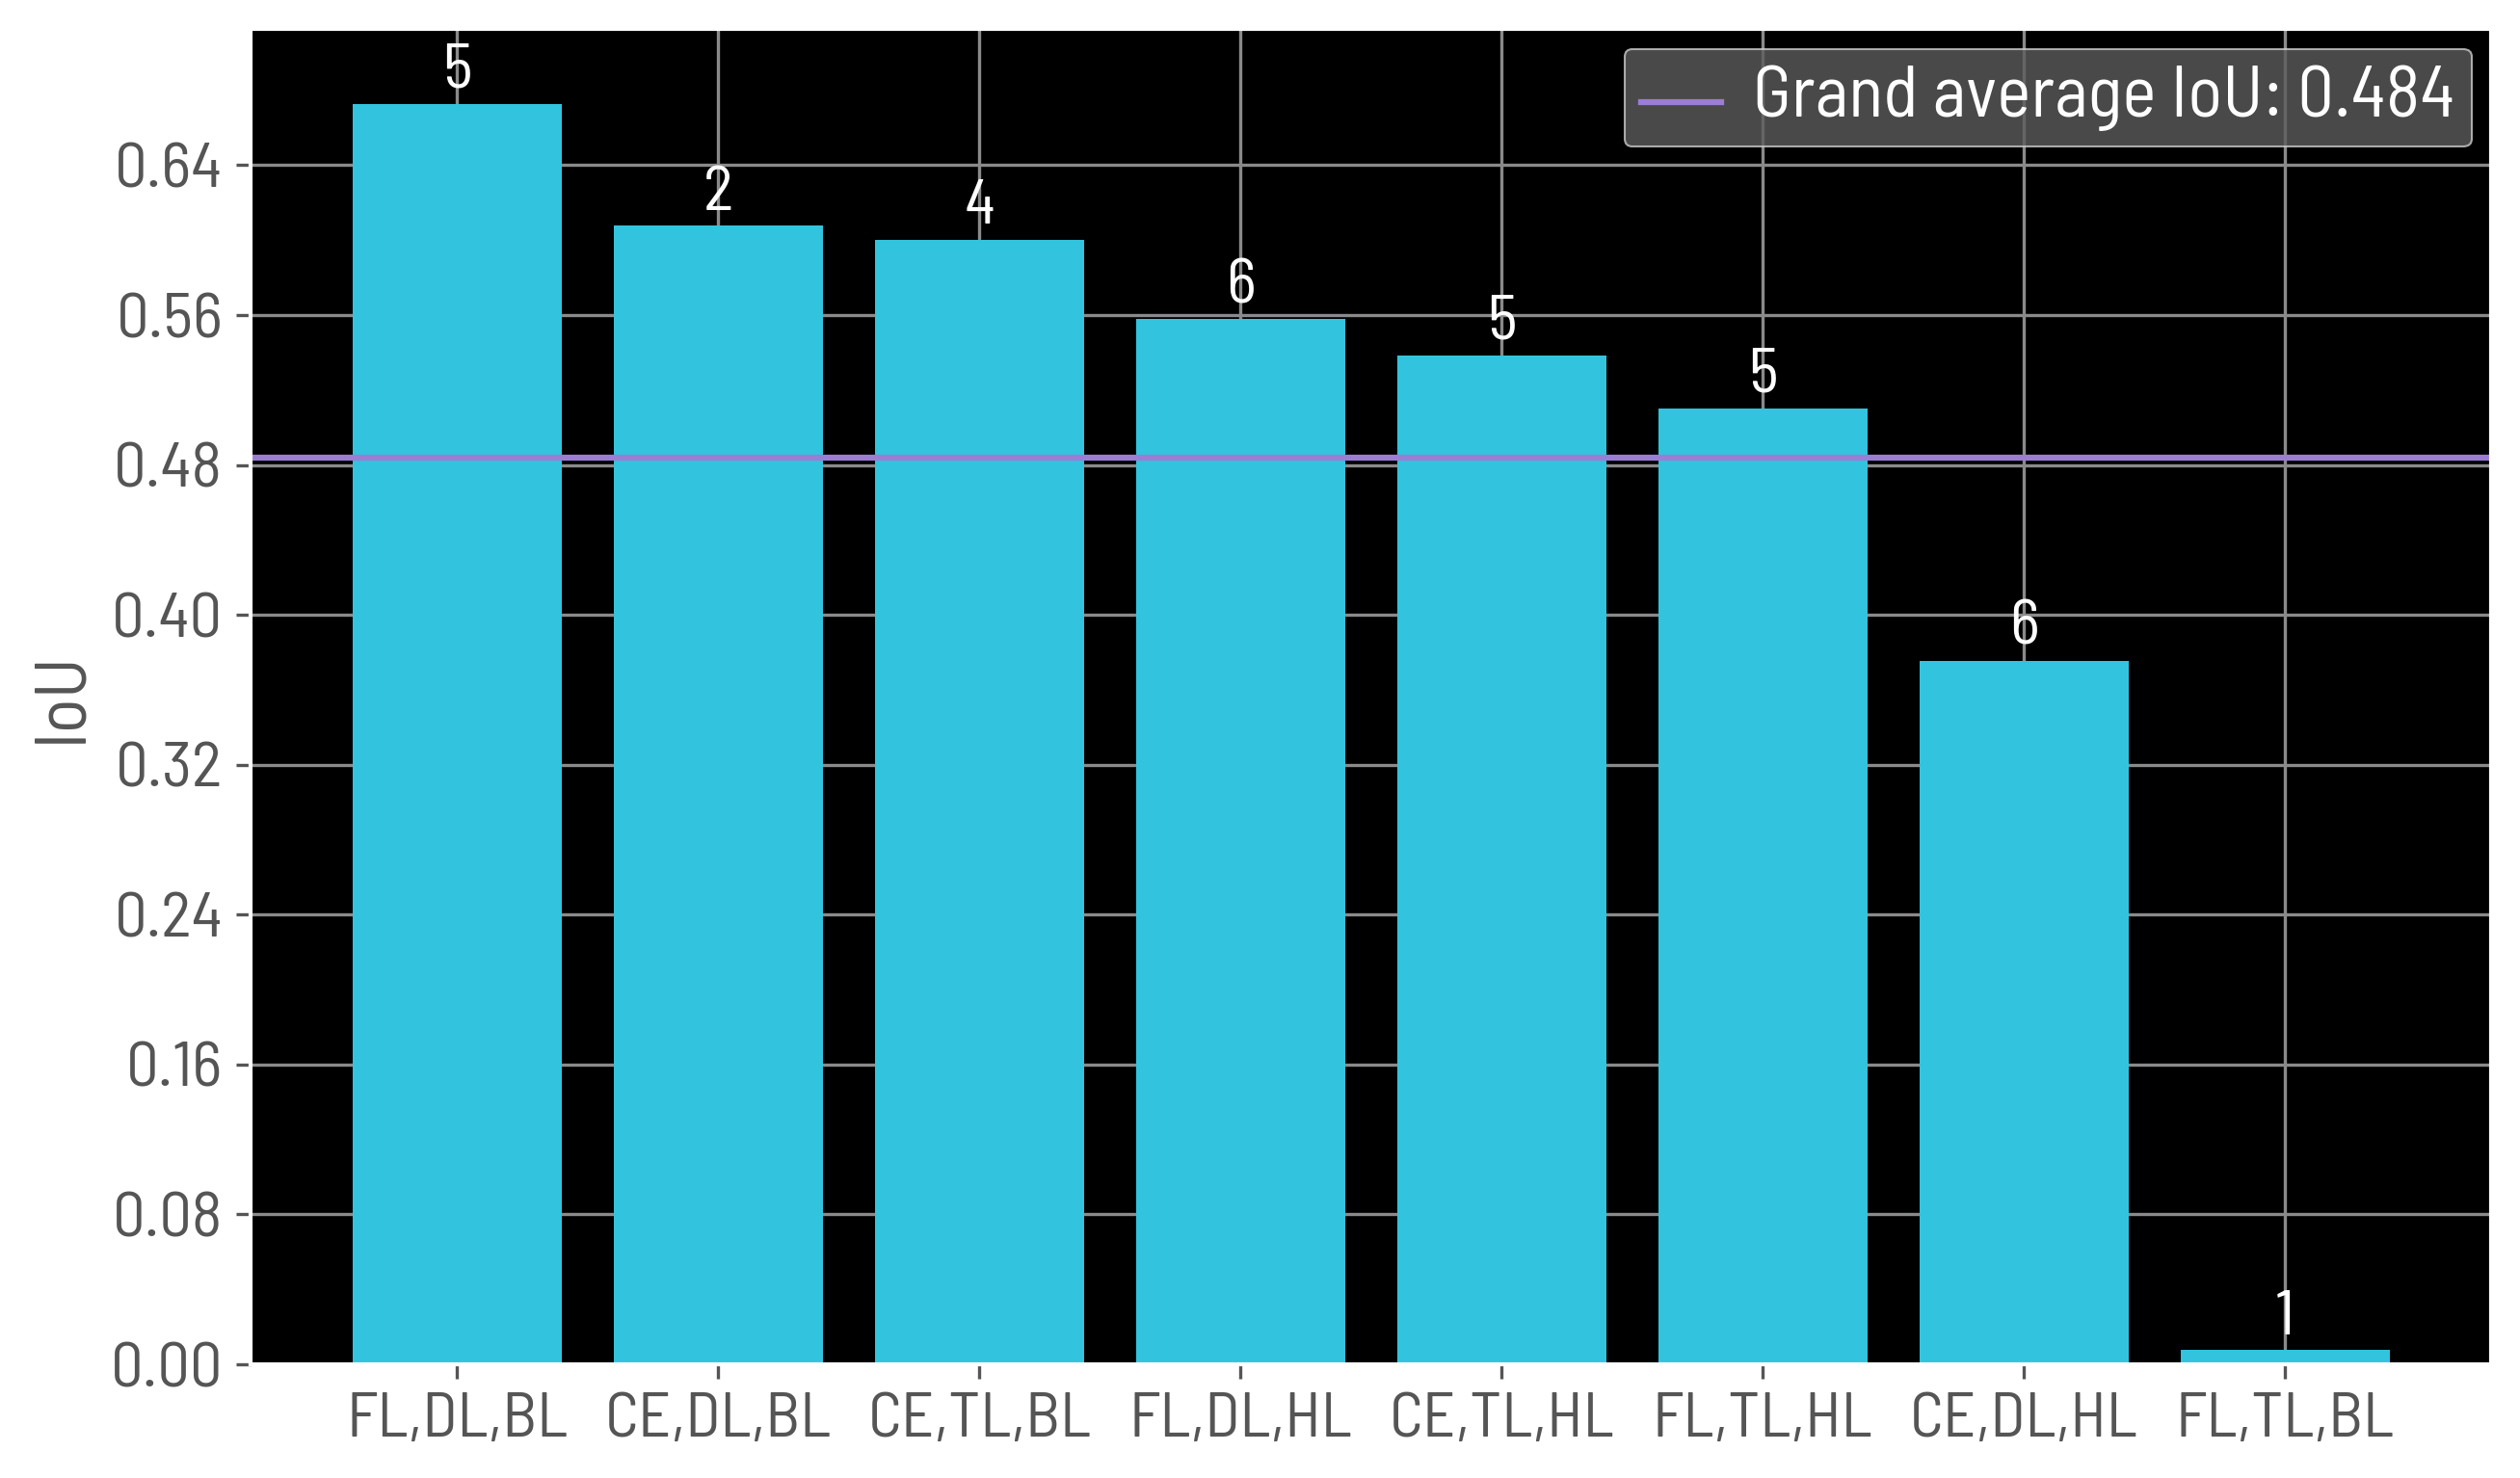
\includegraphics[width=\imgWidthcustom]{images/continous_loss_combination_results_medaka_triple_short_total.png}}
  \caption[Average IoU for Loss Combination (Medaka)]{The figures showcase the average \ac{IoU} for loss combination, derived from an extensive set of 217 models trained on the \ac{MFD} using the performance-based merge strategy.}
  \label{continous_loss_combination_results_medaka_short}
\end{figure}
\figref{continous_results_total_medaka} plots the hyperparameter ranges on the x-axis against the average IoU on the y-axis. Notably, the \texttt{pbm\_I} parameter exhibits a clear trend, wherein a higher value tends to improve performance. By analyzing table \ref{tab:continous_loss_combination_medaka_double_long} and table \ref{tab:continous_loss_combination_medaka_triple_long}, which present the top-performing models generated by the continuous configuration no. 3, we observe that the average \texttt{pbm\_I} value for double loss combinations is 0.755, while for triple loss combinations, it is $0.504$. Additionally, the \texttt{pbm\_alpha} value for these high-performing models was, on average, approximately $6$.
\begin{figure}[H]%[htbp]
  \centering
  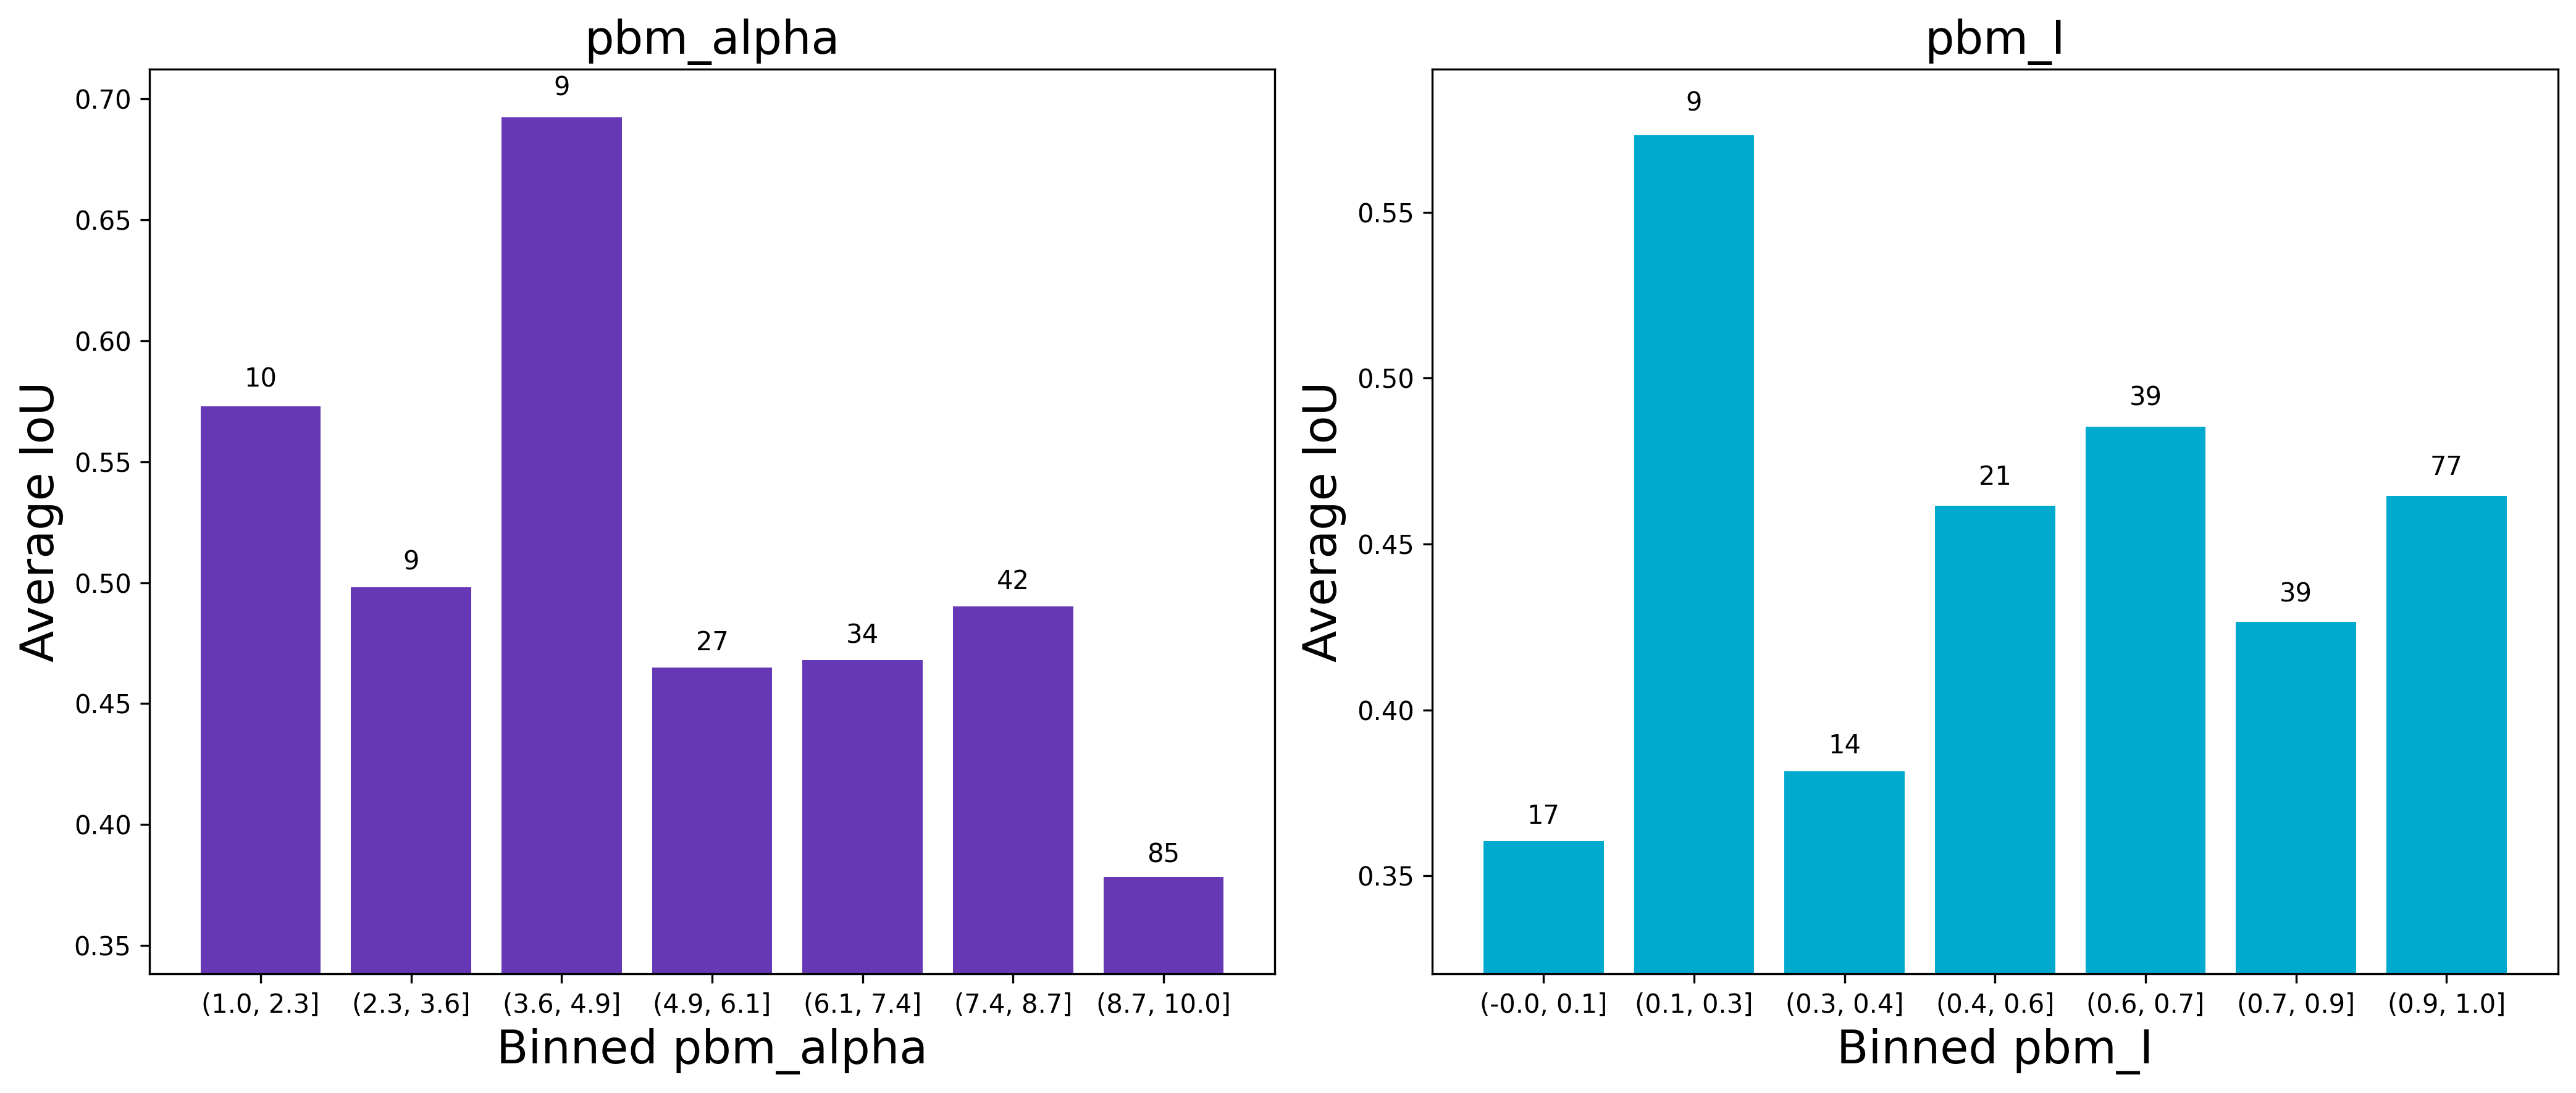
\includegraphics[width=\imgWidthL]{images/continous_hyperparameter_total_medaka.png}
  \caption[Hyperparameter analysis]{Hyperparameter analysis for performance-based merging. The x-axis corresponds to the hyperparameter \texttt{pbm\_alpha} and \texttt{pbm\_I} defined in table \ref{tab:hyperparameters} and \secref{sec:configuration}. Both values are float with \texttt{pbm\_alpha} $\in (1,10]$ and \texttt{pbm\_I}$\in [0,1]$. The bars are labeled with the model count and represent the average \ac{IoU} for the indicated range.}
  \label{continous_results_total_medaka}
\end{figure}

\subsubsection*{Specific Performance}
As a specific loss-merge combination for the specific configuration no.5 defined in table \ref{tab:final_configuration_list}, the PBM strategy along the combinations of \ac{FL},\ac{DL} and \ac{BL} was used, and resulted in a grand average of $0.695$ for 18 models trained, surpassing the continuous average by 2.5\% as well as the best average baseline implementation by 2.3\%. The detailed results for each model can be viewed in \secref{subsec:specific_combination_medaka}.

%----------------------------------------------------------------------------------------%
%---------------------------------------Skin Lesion--------------------------------------%
%----------------------------------------------------------------------------------------%
\subsection{Skin Lesion}
\label{subsec:skin_lesion}
This second dataset comprises dermoscopic images of skin lesions, as described in more detail in \secref{sec:datasets}. The dataset consists of two classes: foreground and background. Configurations 6 to 9 from table \ref{tab:final_configuration_list} were used for this dataset, including the baseline, one discrete, one continuous and the specific configuration, similar to the \ac{MFD}.

%------------------------------BASELINE PERFORMANCE (Skin Lesion)------------------------%
\subsubsection*{Baseline Performance}
\label{subsubsec:baseline_performance_skin_lesion}
Table \ref{tab:baseline_skin_lesion_short} summarizes the baseline results for the \ac{SLD}. Each row represents the average performance by the loss function. This baseline average was created using configuration no. 6 defined in \secref{sec:configuration}. This configuration underwent six training rounds for a reliable performance assessment, leading to the development of 108 models. The final column of the table, \squote{\ac{PPV} vs. \ac{TPR}}, determines whether a scenario presents high precision with low recall or low precision with high recall.

\textbf{Distribution-based results}\newline
Although a model trained with the \ac{CE} achieved the highest score among all models, see \ref{tab:baseline_skin_lesion_long} (No. 1), the average result over nine models was 3.7\% lower than the average trained with the \ac{FL}. Interestingly, none of the top-performing \ac{CE} models used the entire dataset but subsets of 64 and 32\%. All models that used the entire dataset for training resulted in an average of 14.7\% lower than the top-performing model, which only used 64\% of the data. See table \ref{tab:baseline_skin_lesion_long} for further information on the top-performing models.

The \ac{FL} achieved an average \ac{IoU} of $0.594$ across the 18 baseline models. The best-performing model trained with the \ac{FL} scored $0.666$, nearly as good as the overall best-performing model. As expected, most top-performing models trained with the \ac{FL} used the entire dataset.

\textbf{Region-based results}\newline
The \ac{DL} achieved an average \ac{IoU} of $0.560$, resulting in a performance decrease of 3.4\% compared to the \ac{FL} average. Among the region-based losses, the \ac{TL} achieved slightly better performance with an \ac{IoU} of $0.574$. Even if the average \ac{TPR} of the \ac{TL} did not top the average results of \ac{FL} and \ac{DL}, it still represents the top-performing model in terms of \ac{TPR}, demonstrating its intended function as described in \cite{DBLP:journals/corr/SalehiEG17a}. See result table \ref{tab:baseline_skin_lesion_long} (No. 28).

\textbf{Boundary-based results}\newline
Among the boundary-based loss functions, the \ac{HL} achieved an average \ac{IoU} of $0.542$ and the \ac{BL} an average \ac{IoU} of $0.287$ which seemed to have been converging for this dataset but still lacks meaningful results compared to other loss functions used.

% Please add the following required packages to your document preamble:
% \usepackage[table,xcdraw]{xcolor}
% If you use beamer only pass "xcolor=table" option, i.e. \documentclass[xcolor=table]{beamer}
\begin{table}[H]
  \centering
  \begin{tabular}{cc|l|l|l|l|c|}
  \hline
  \rowcolor[HTML]{000000} 
  \multicolumn{1}{|c|}{\cellcolor[HTML]{000000}{\color[HTML]{FFFFFF} No.}} &
    {\color[HTML]{FFFFFF} Loss type} &
    {\color[HTML]{FFFFFF} Loss} &
    \multicolumn{1}{c|}{\cellcolor[HTML]{000000}{\color[HTML]{FFFFFF} IoU}} &
    \multicolumn{1}{c|}{\cellcolor[HTML]{000000}{\color[HTML]{FFFFFF} PPV}} &
    \multicolumn{1}{c|}{\cellcolor[HTML]{000000}{\color[HTML]{FFFFFF} TPR}} &
    {\color[HTML]{FFFFFF} PPV vs. TPR} \\ \hline
  \multicolumn{1}{|c|}{{\color[HTML]{000000} 1}} &
    \cellcolor[HTML]{6638B6}{\color[HTML]{FFFFFF} DB} &
    {\color[HTML]{000000} CE} &
    {\color[HTML]{000000} 0.557} &
    {\color[HTML]{000000} 0.753} &
    {\color[HTML]{000000} 0.682} &
    {\color[HTML]{000000} PPV} \\ \hline
  \multicolumn{1}{|c|}{{\color[HTML]{000000} \textit{\textbf{2}}}} &
    \cellcolor[HTML]{6638B6}{\color[HTML]{FFFFFF} \textit{\textbf{DB}}} &
    {\color[HTML]{000000} \textit{\textbf{FL}}} &
    {\color[HTML]{000000} \textit{\textbf{0.594}}} &
    {\color[HTML]{000000} \textit{\textbf{0.792}}} &
    {\color[HTML]{000000} \textit{\textbf{0.723}}} &
    {\color[HTML]{000000} \textit{\textbf{PPV}}} \\ \hline
  \multicolumn{1}{|c|}{{\color[HTML]{000000} 3}} &
    \cellcolor[HTML]{00A9CE}{\color[HTML]{FFFFFF} RB} &
    {\color[HTML]{000000} DL} &
    {\color[HTML]{000000} 0.560} &
    {\color[HTML]{000000} 0.739} &
    {\color[HTML]{000000} 0.714} &
    {\color[HTML]{000000} PPV} \\ \hline
  \multicolumn{1}{|c|}{{\color[HTML]{000000} 4}} &
    \cellcolor[HTML]{00A9CE}{\color[HTML]{FFFFFF} RB} &
    {\color[HTML]{000000} TL} &
    {\color[HTML]{000000} 0.574} &
    {\color[HTML]{000000} 0.751} &
    {\color[HTML]{000000} 0.713} &
    {\color[HTML]{000000} PPV} \\ \hline
  \multicolumn{1}{|c|}{{\color[HTML]{000000} 5}} &
    \cellcolor[HTML]{99DDFD}{\color[HTML]{FFFFFF} BB} &
    {\color[HTML]{000000} HL\textsubscript{1}} &
    {\color[HTML]{000000} 0.542} &
    {\color[HTML]{000000} 0.750} &
    {\color[HTML]{000000} 0.677} &
    {\color[HTML]{000000} PPV} \\ \hline
  \multicolumn{1}{|c|}{{\color[HTML]{000000} 6}} &
    \cellcolor[HTML]{99DDFD}{\color[HTML]{FFFFFF} BB} &
    {\color[HTML]{000000} BL} &
    {\color[HTML]{000000} 0.287} &
    {\color[HTML]{000000} 0.519} &
    {\color[HTML]{000000} 0.520} &
    {\color[HTML]{000000} TPR} \\ \hline
  {\color[HTML]{000000} } &
    {\color[HTML]{000000} } &
    \cellcolor[HTML]{000000}{\color[HTML]{FFFFFF} \textit{\textbf{Grand Average}}} &
    \cellcolor[HTML]{000000}{\color[HTML]{FFFFFF} \textit{\textbf{0.512}}} &
    \cellcolor[HTML]{000000}{\color[HTML]{FFFFFF} \textit{\textbf{0.712}}} &
    \cellcolor[HTML]{000000}{\color[HTML]{FFFFFF} \textit{\textbf{0.666}}} &
    \cellcolor[HTML]{000000}{\color[HTML]{FFFFFF} \textit{\textbf{PPV}}} \\ \cline{3-7} 
  \end{tabular}
  \caption[Overall baseline results for the Skin Lesion dataset]{The table presents a summary of the average values of various metrics for six baseline models trained for each loss function and each selection percentage. The total number of models trained for this baseline result is 108. The column titled \squote{PPV vs. TPR} illustrates the trade-off between a high \acf{PPV} and low \acf{TPR}, or vice versa, for each model.}
  \label{tab:baseline_skin_lesion_short}
  \end{table}

%----------------------------------OVERALL PERFORMANCE (Skin Lesion)---------------------%
\subsubsection*{Overall Performance}
\label{subsubsec:skin_lesion_overall_performance}
The pair of heatmaps illustrated below portray the cumulative results obtained from the \ac{SLD}, which was generated via the execution of configurations 7 and 8 as defined in \ref{tab:final_configuration_list}. Specifically, discrete configuration no. 7 led to the training of 360 models, while continuous configuration no. 8 contributed an additional 146 models, thereby yielding a total of 506 models.

It is important to note that while the model count for the discrete configuration is predetermined, the continuous configuration necessitates an exploration of an array of hyperparameters. This exploration is facilitated by the Hyperband algorithm, which strategically favors promising combinations while simultaneously discarding those that demonstrate inferior performance. In this context, \squote{combination} refers to integrating loss combinations, merge strategies, and their corresponding hyperparameters.

The relatively fewer models used for the continuous configuration within this dataset can be attributed to its substantial size. Specifically, the training set of the \ac{SLD} is approximately 3.5 times larger than that of the \ac{MFD}. Consequently, it demands significantly greater computational resources and time, hence the more limited model use in the continuous configuration.

\begin{figure}[H]%[htbp]
  \centering
  \subfigure[Overall performance of double combinations]{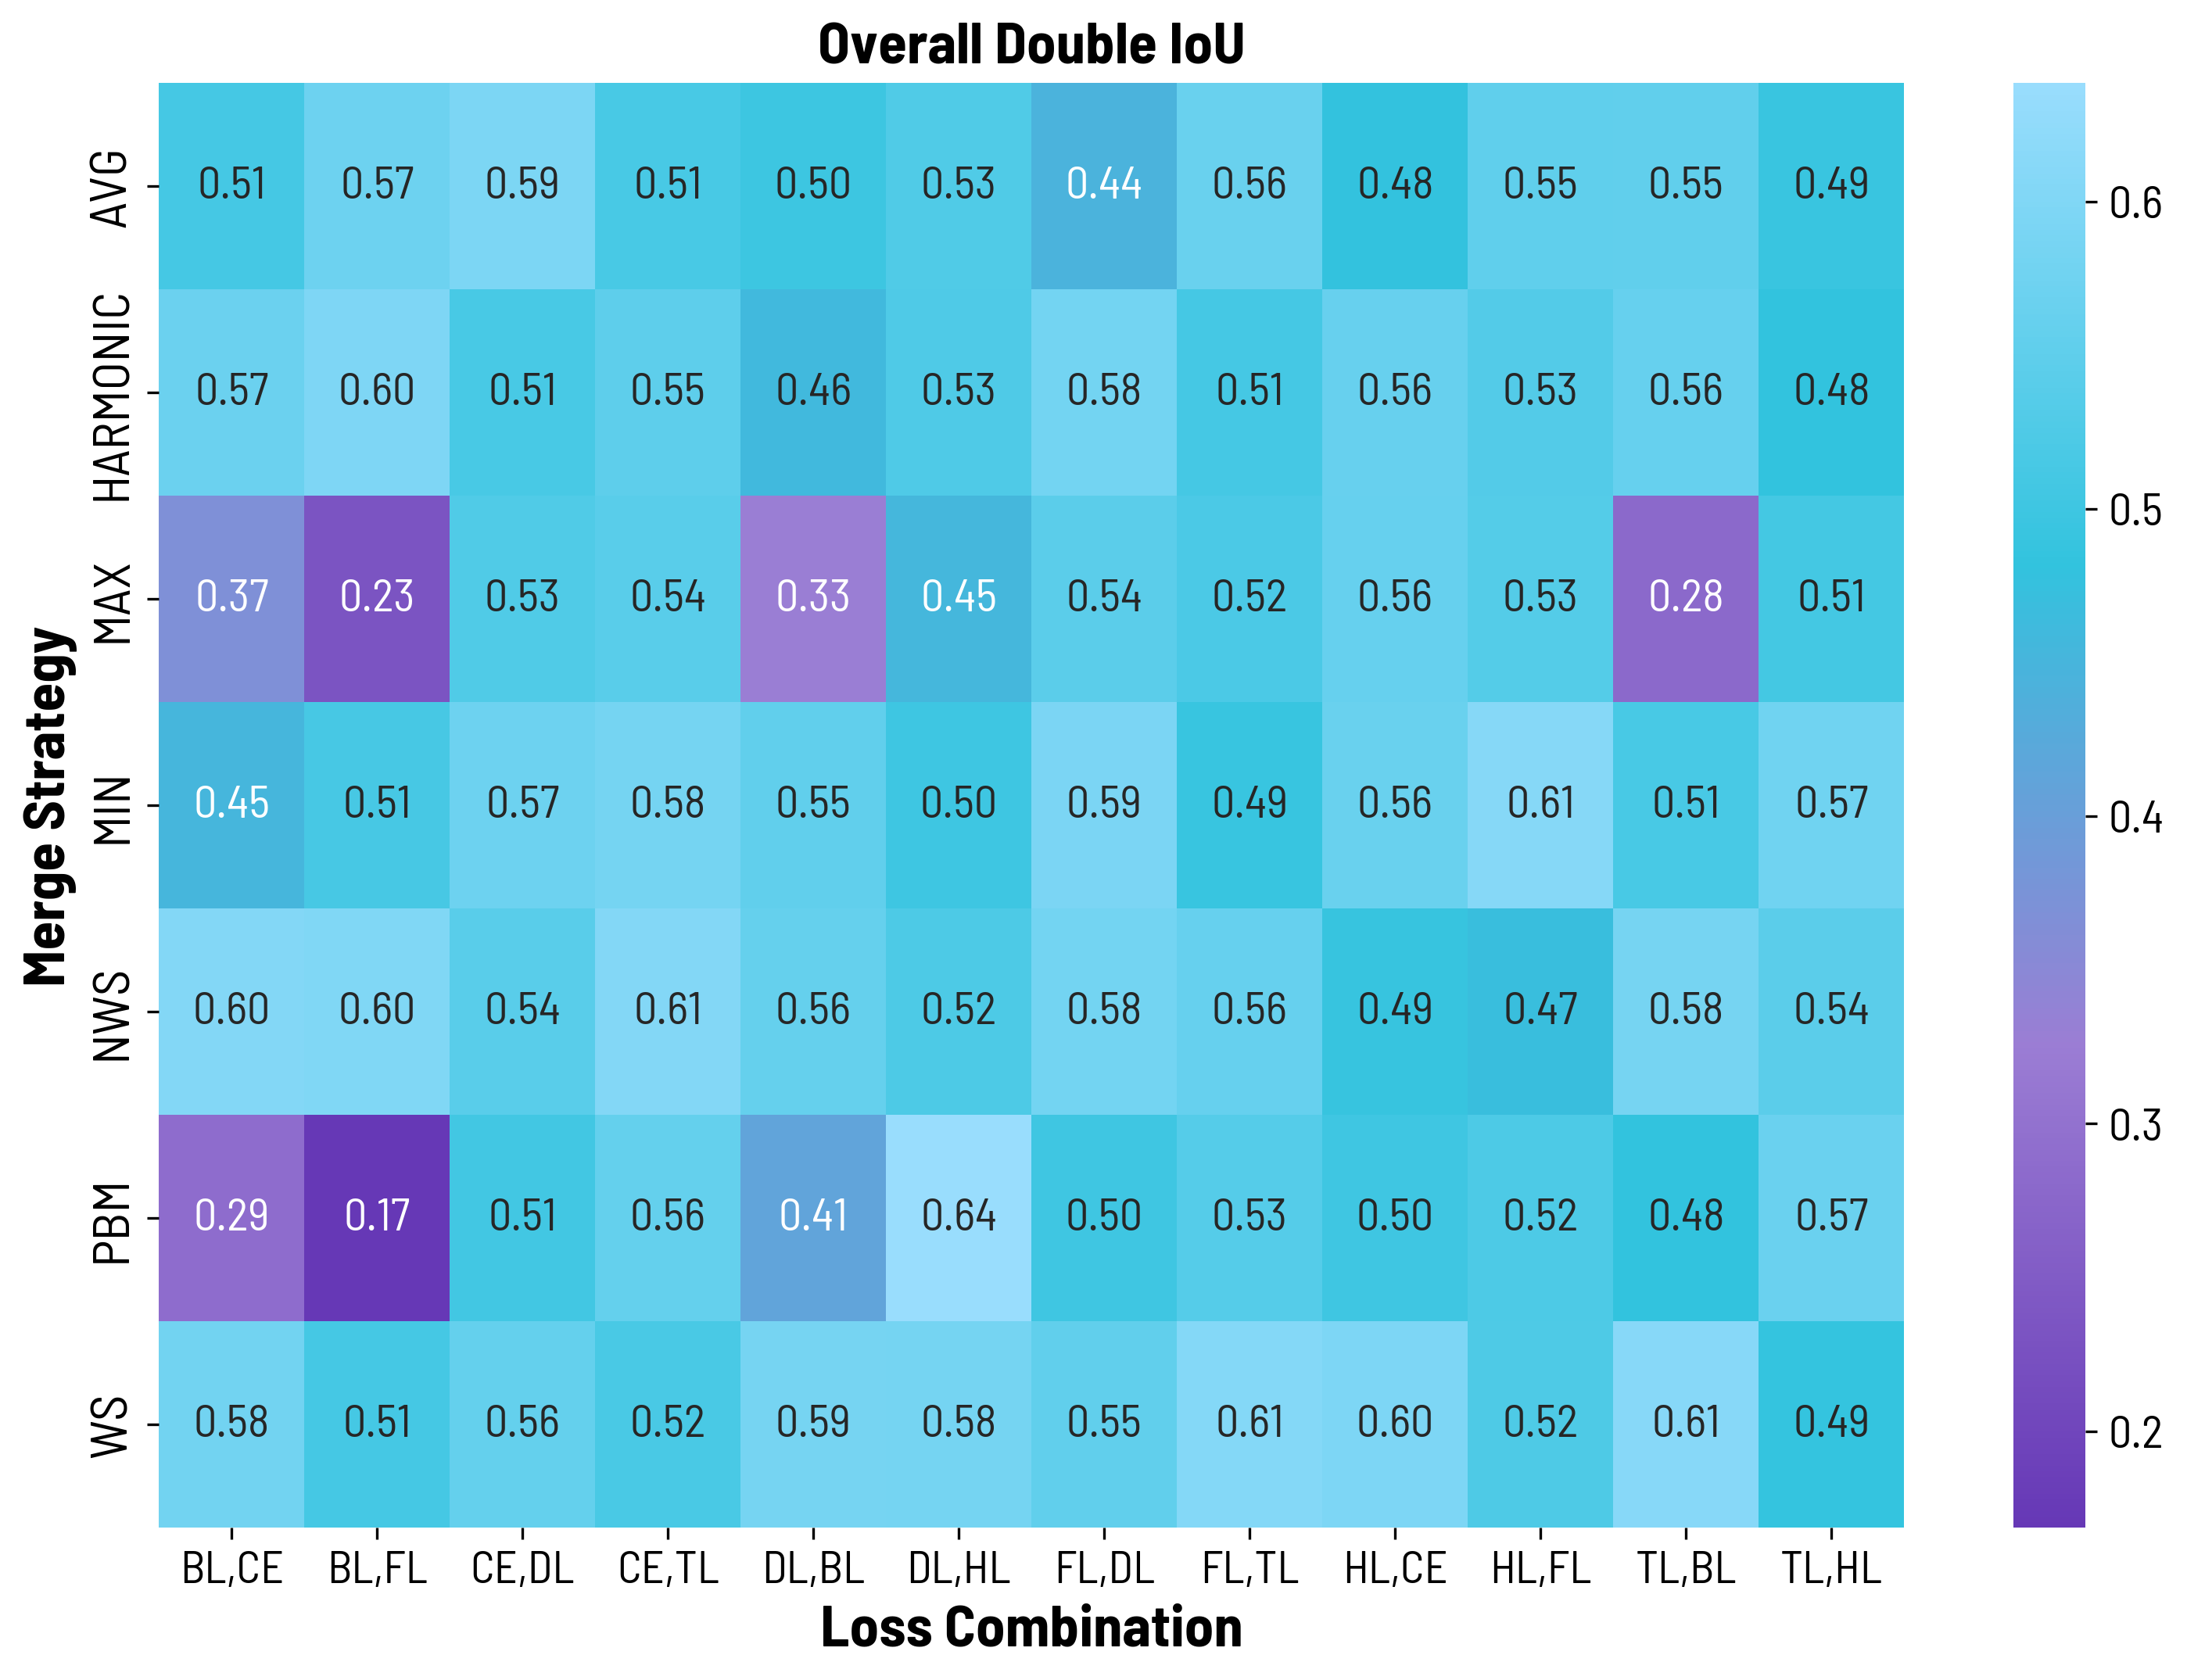
\includegraphics[width=\imgWidthcustom]{images/overall_results_double_melanoma.png}}
  \subfigure[Overall performance of triple combinations]{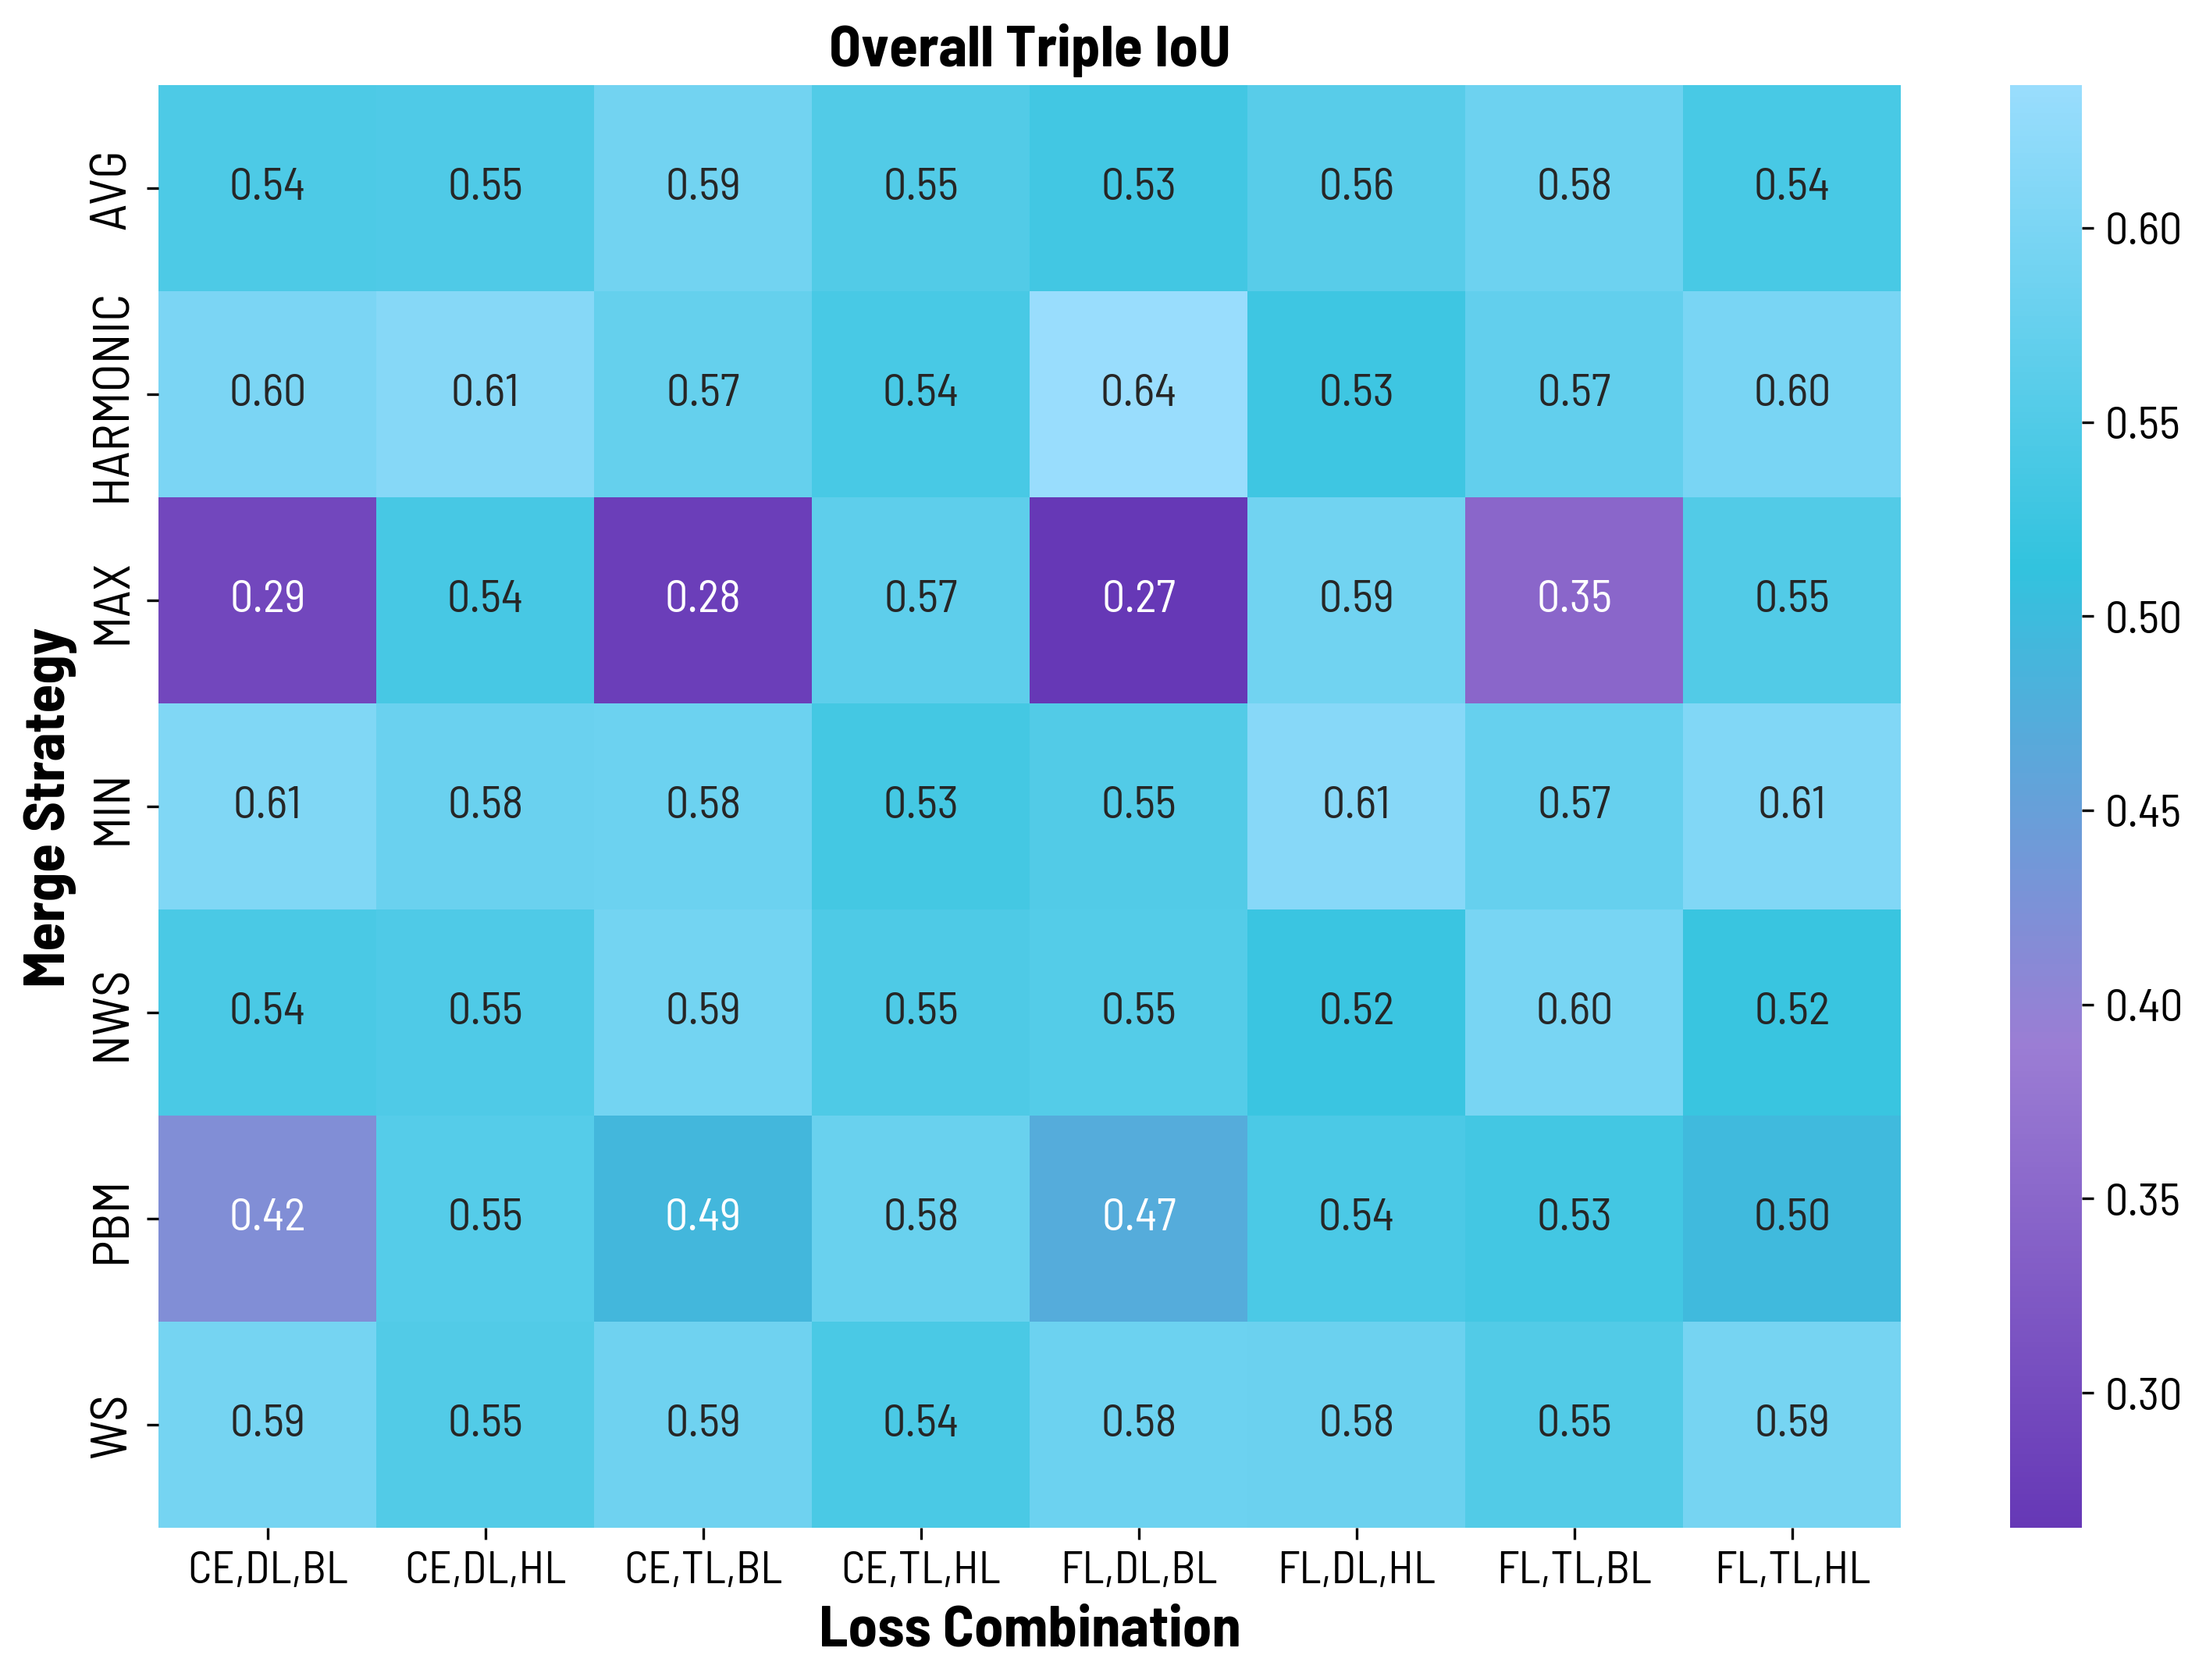
\includegraphics[width=\imgWidthcustom]{images/overall_results_triple_melanoma.png}}
  \caption[Overall performance of triple combinations]{Average \ac{IoU} for all double and triple loss-merge combinations.}
  \label{overall_double_triple_melanoma}
\end{figure}
Analyzing the two heatmaps depicted in \figref{overall_double_triple_melanoma}, it becomes apparent that all merging strategies, except for MAX and PBM, display good results for this specific dataset. Two combinations stand out above the rest: firstly, the DL, HL loss combined with the PBM strategy for double loss combinations, and secondly, the FL, DL, BL combination with the HARMONIC strategy for triple combinations. Given PBM's generally low average performance, the former combination's high performance might be an outlier, requiring further examination. In contrast, the success of the latter combination appears more consistent, mainly due to the overall decent performance of the HARMONIC strategy.

%----------------------------------DISCRETE PERFORMANCE (Skin Lesion)--------------------%
\subsubsection*{Discrete Performance}
This subsection analyzes the discrete configuration no. 7 exclusively from a loss combination and merge strategy perspective. The average results are generally the average of the respective columns and rows of the two heatmaps presented above.

\textbf{Loss combination results}\newline
\figref{loss_combination_results_melanoma_short} displays the average result of 360 models, each trained using a different loss combination. Image (a) showcases all dual loss combinations, while image (b) exhibits all triple loss combinations arranged in descending order by \ac{IoU}. As observed with the \ac{MFD}, combinations involving the \ac{BL} performed below the grand average for both dual and triple combinations. For dual loss combinations, distribution and region-based losses outperformed others, although some combinations with the \ac{HL} also yielded decent results.
\begin{figure}[H]%[htbp]
  \centering
  \subfigure[Average IoU for Each Double Loss Combination]{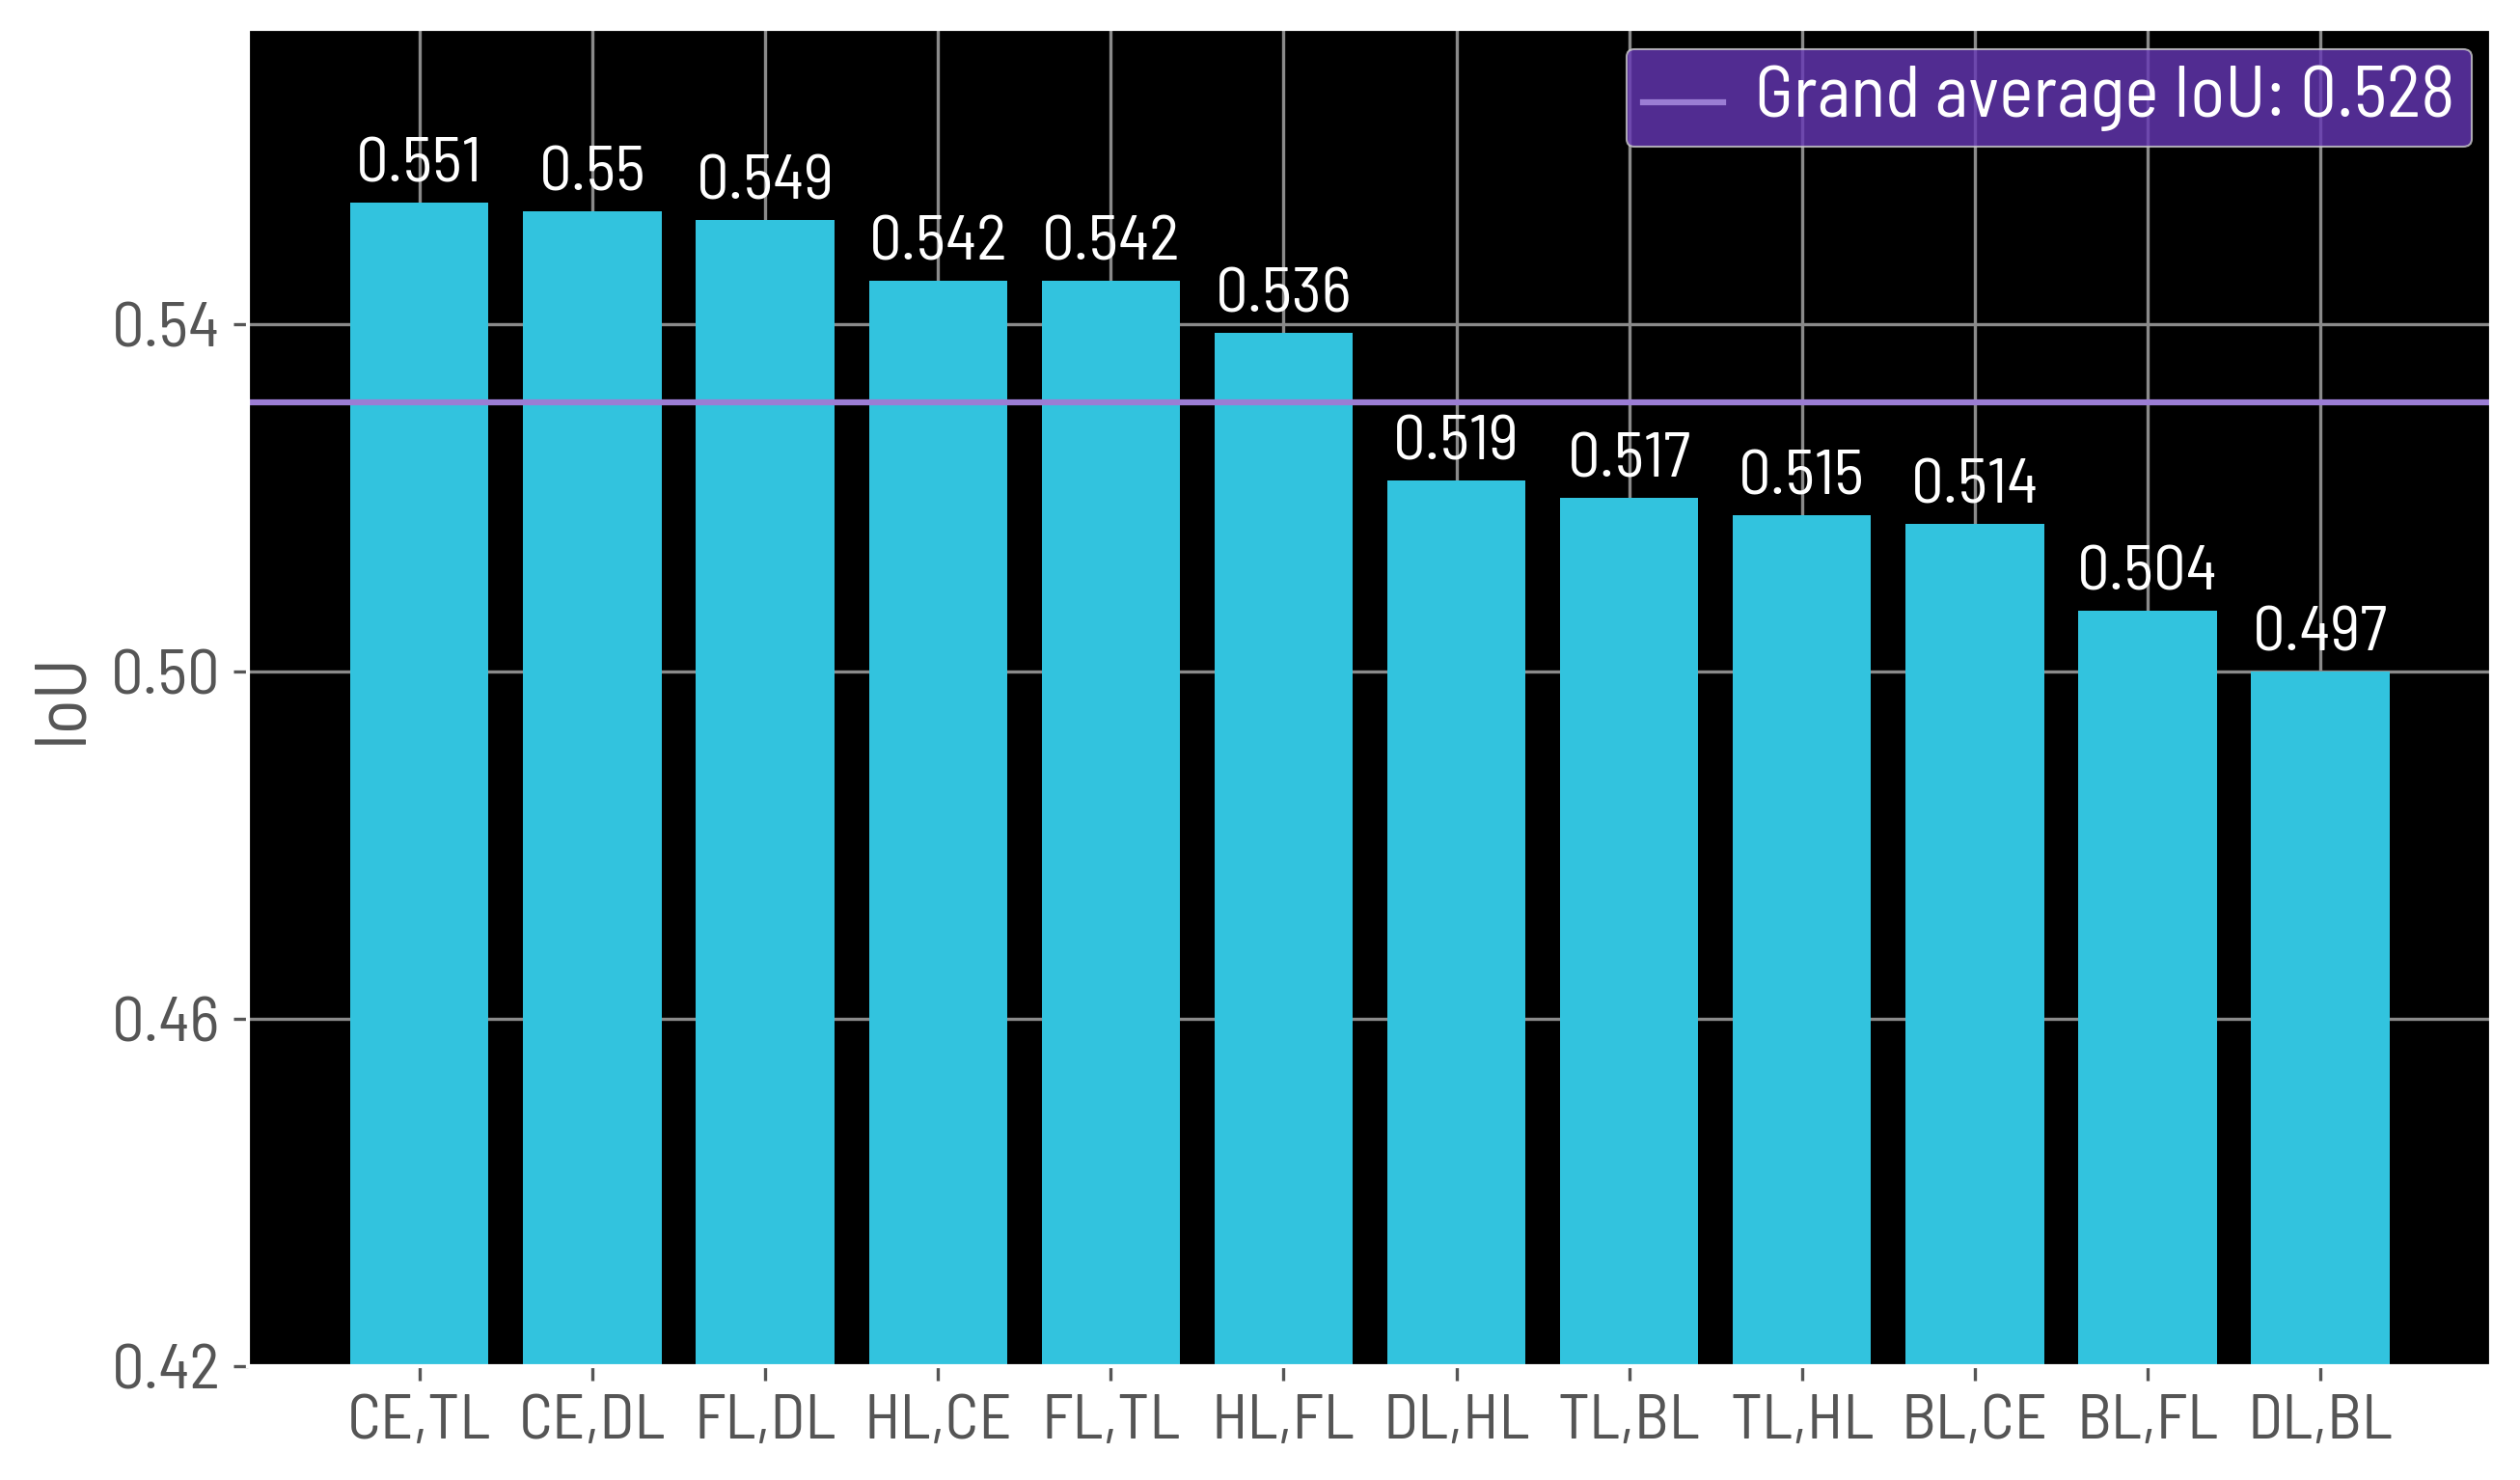
\includegraphics[width=\imgWidthcustom]{images/loss_combination_results_melanoma_double_short_total.png}}
  \subfigure[Average IoU for Each Triple Loss Combination]{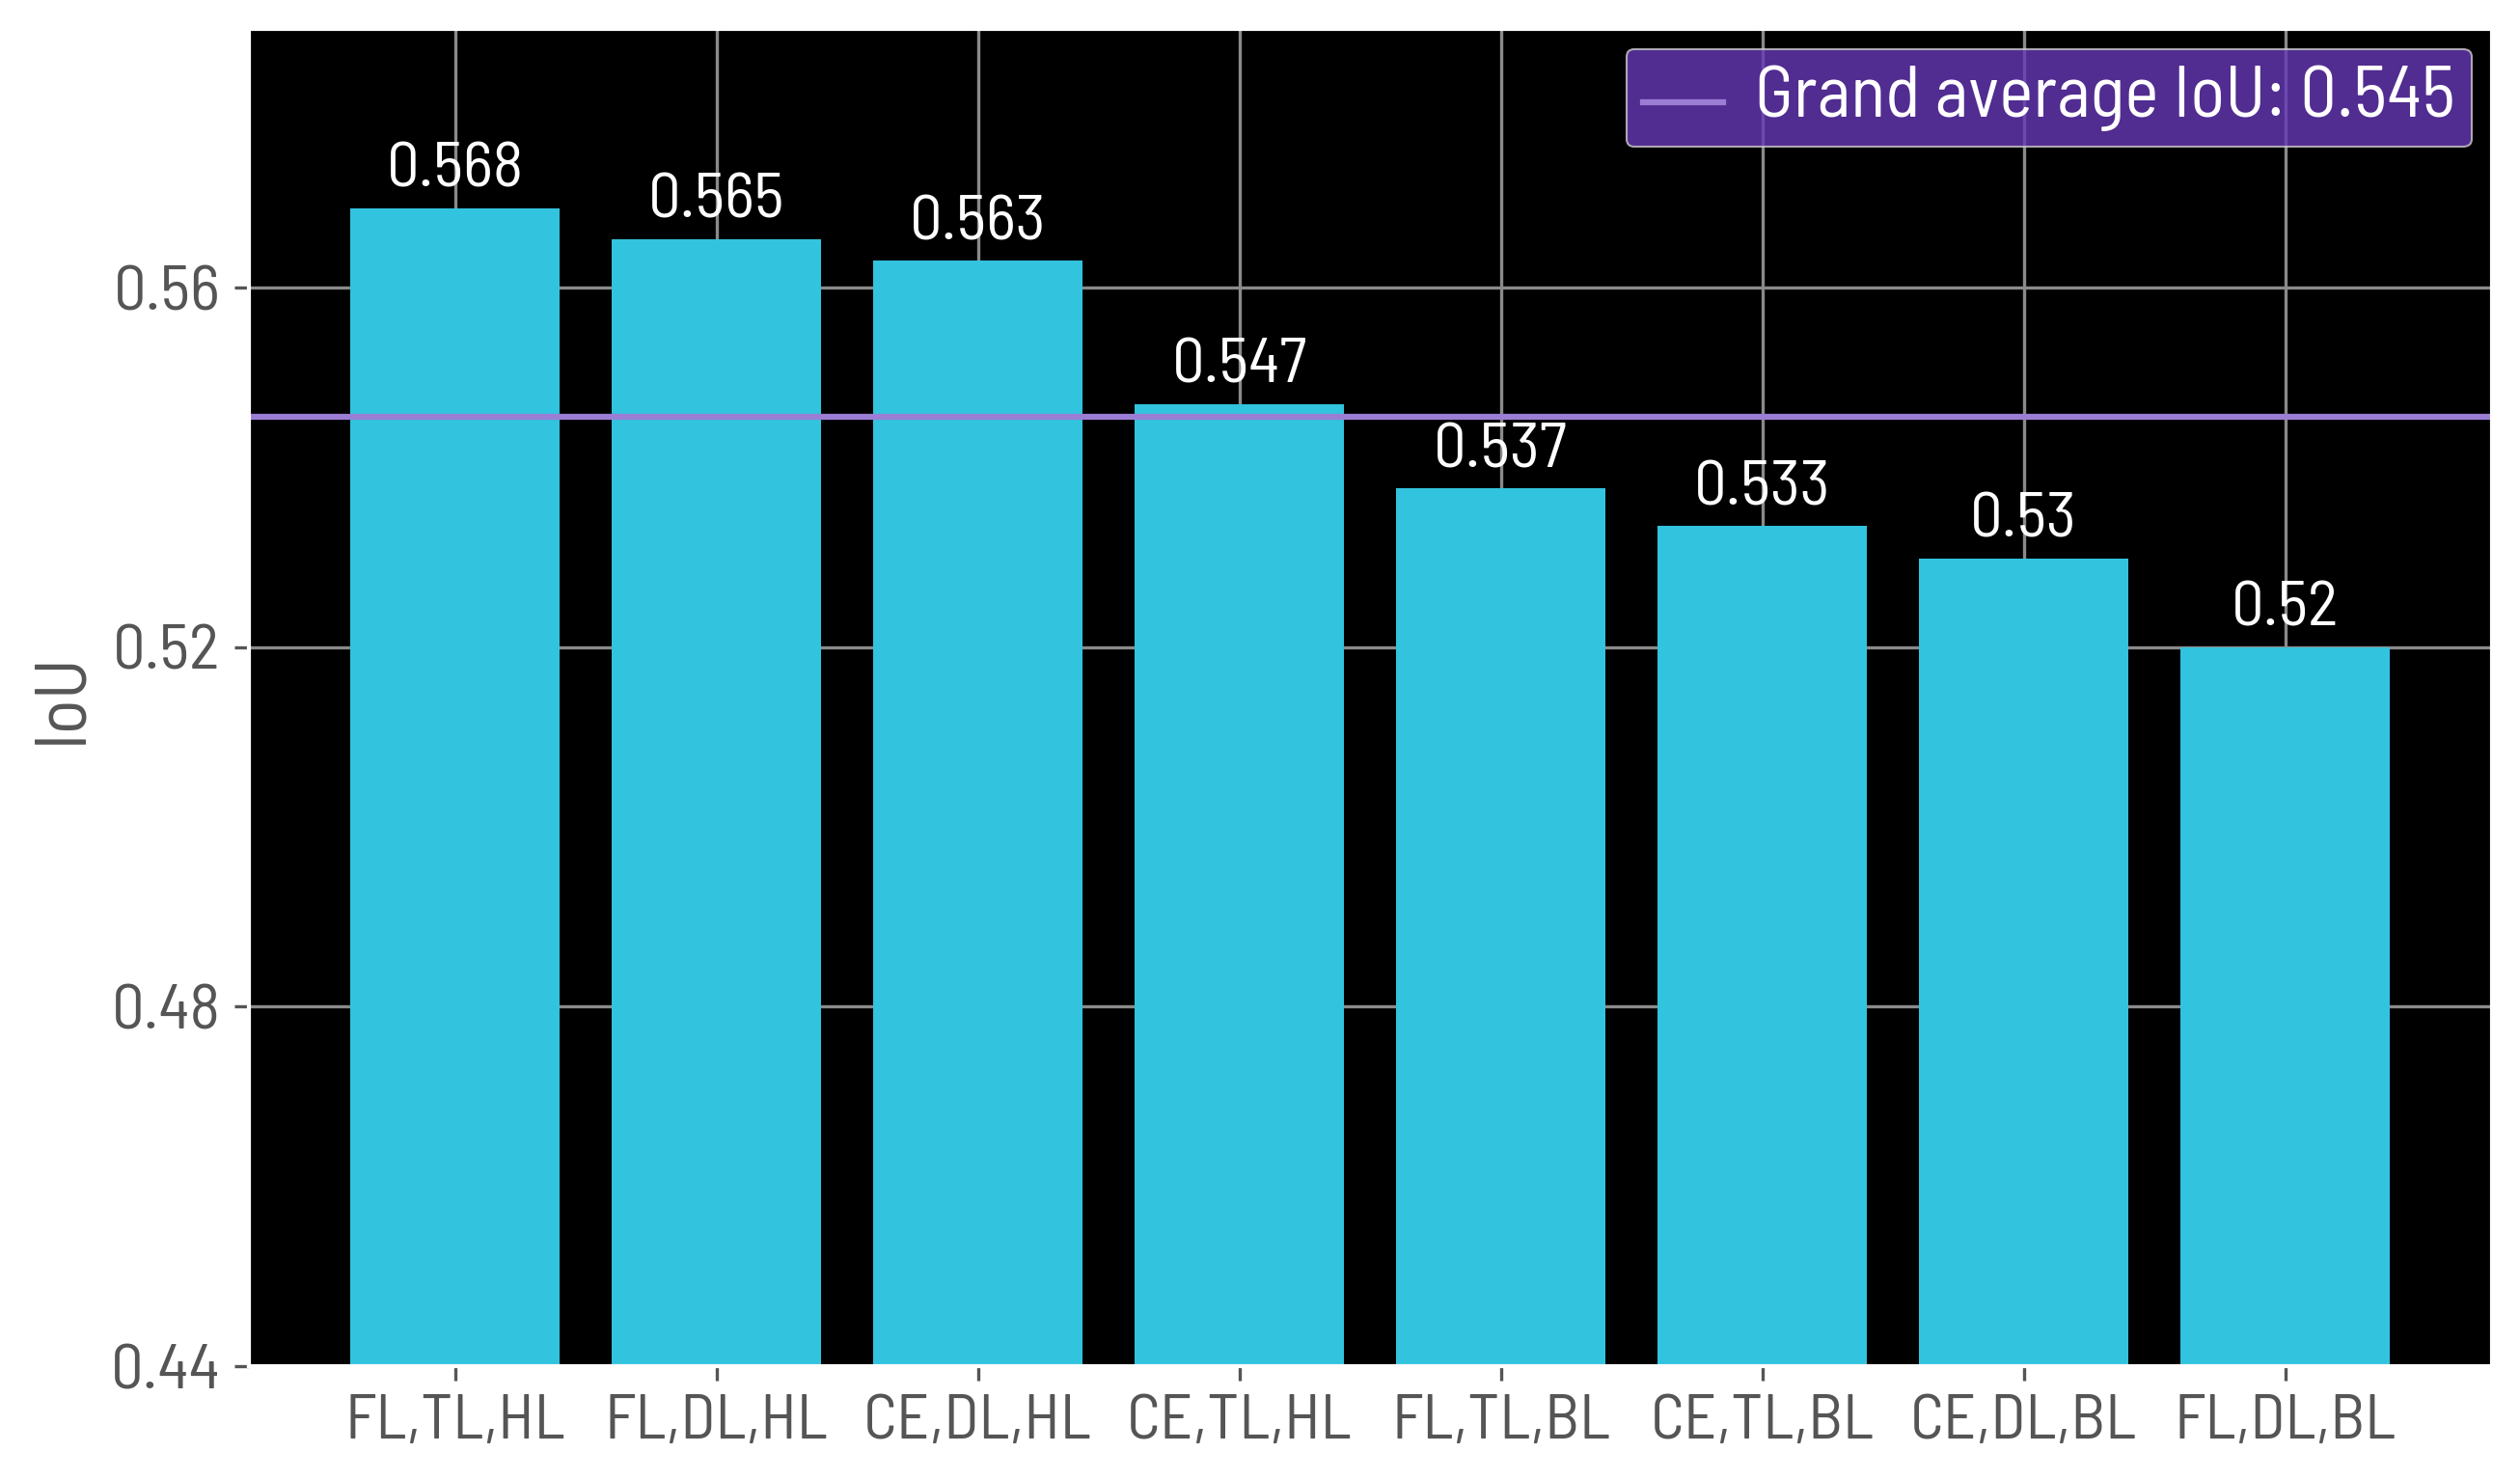
\includegraphics[width=\imgWidthcustom]{images/loss_combination_results_melanoma_triple_short_total.png}}
  \caption[Average IoU for Loss Combination (Skin Lesion)]{The figures showcase the average \ac{IoU} for loss combination, as well as their corresponding selection percentages, derived from an extensive set of 360 models trained on the \ac{SLD}.}
  \label{loss_combination_results_melanoma_short}
\end{figure}

\textbf{Merge strategy results}\newline
\figref{merge_strategy_results_melanoma_short} displays the average performance categorized by merge strategy. In the case of the Medaka Fish, the AVG strategy ranked among the top strategies for all loss combinations. However, for the \ac{SLD}, AVG only reached the fifth position for dual loss combinations and the fourth for triple loss combinations. Meanwhile, the static weighting strategies, WS and NWS, showed stable performance on average for both dual and triple loss combinations.
\begin{figure}[H]%[htbp]
  \centering
  \subfigure[Average IoU for Each Double Merge Strategy]{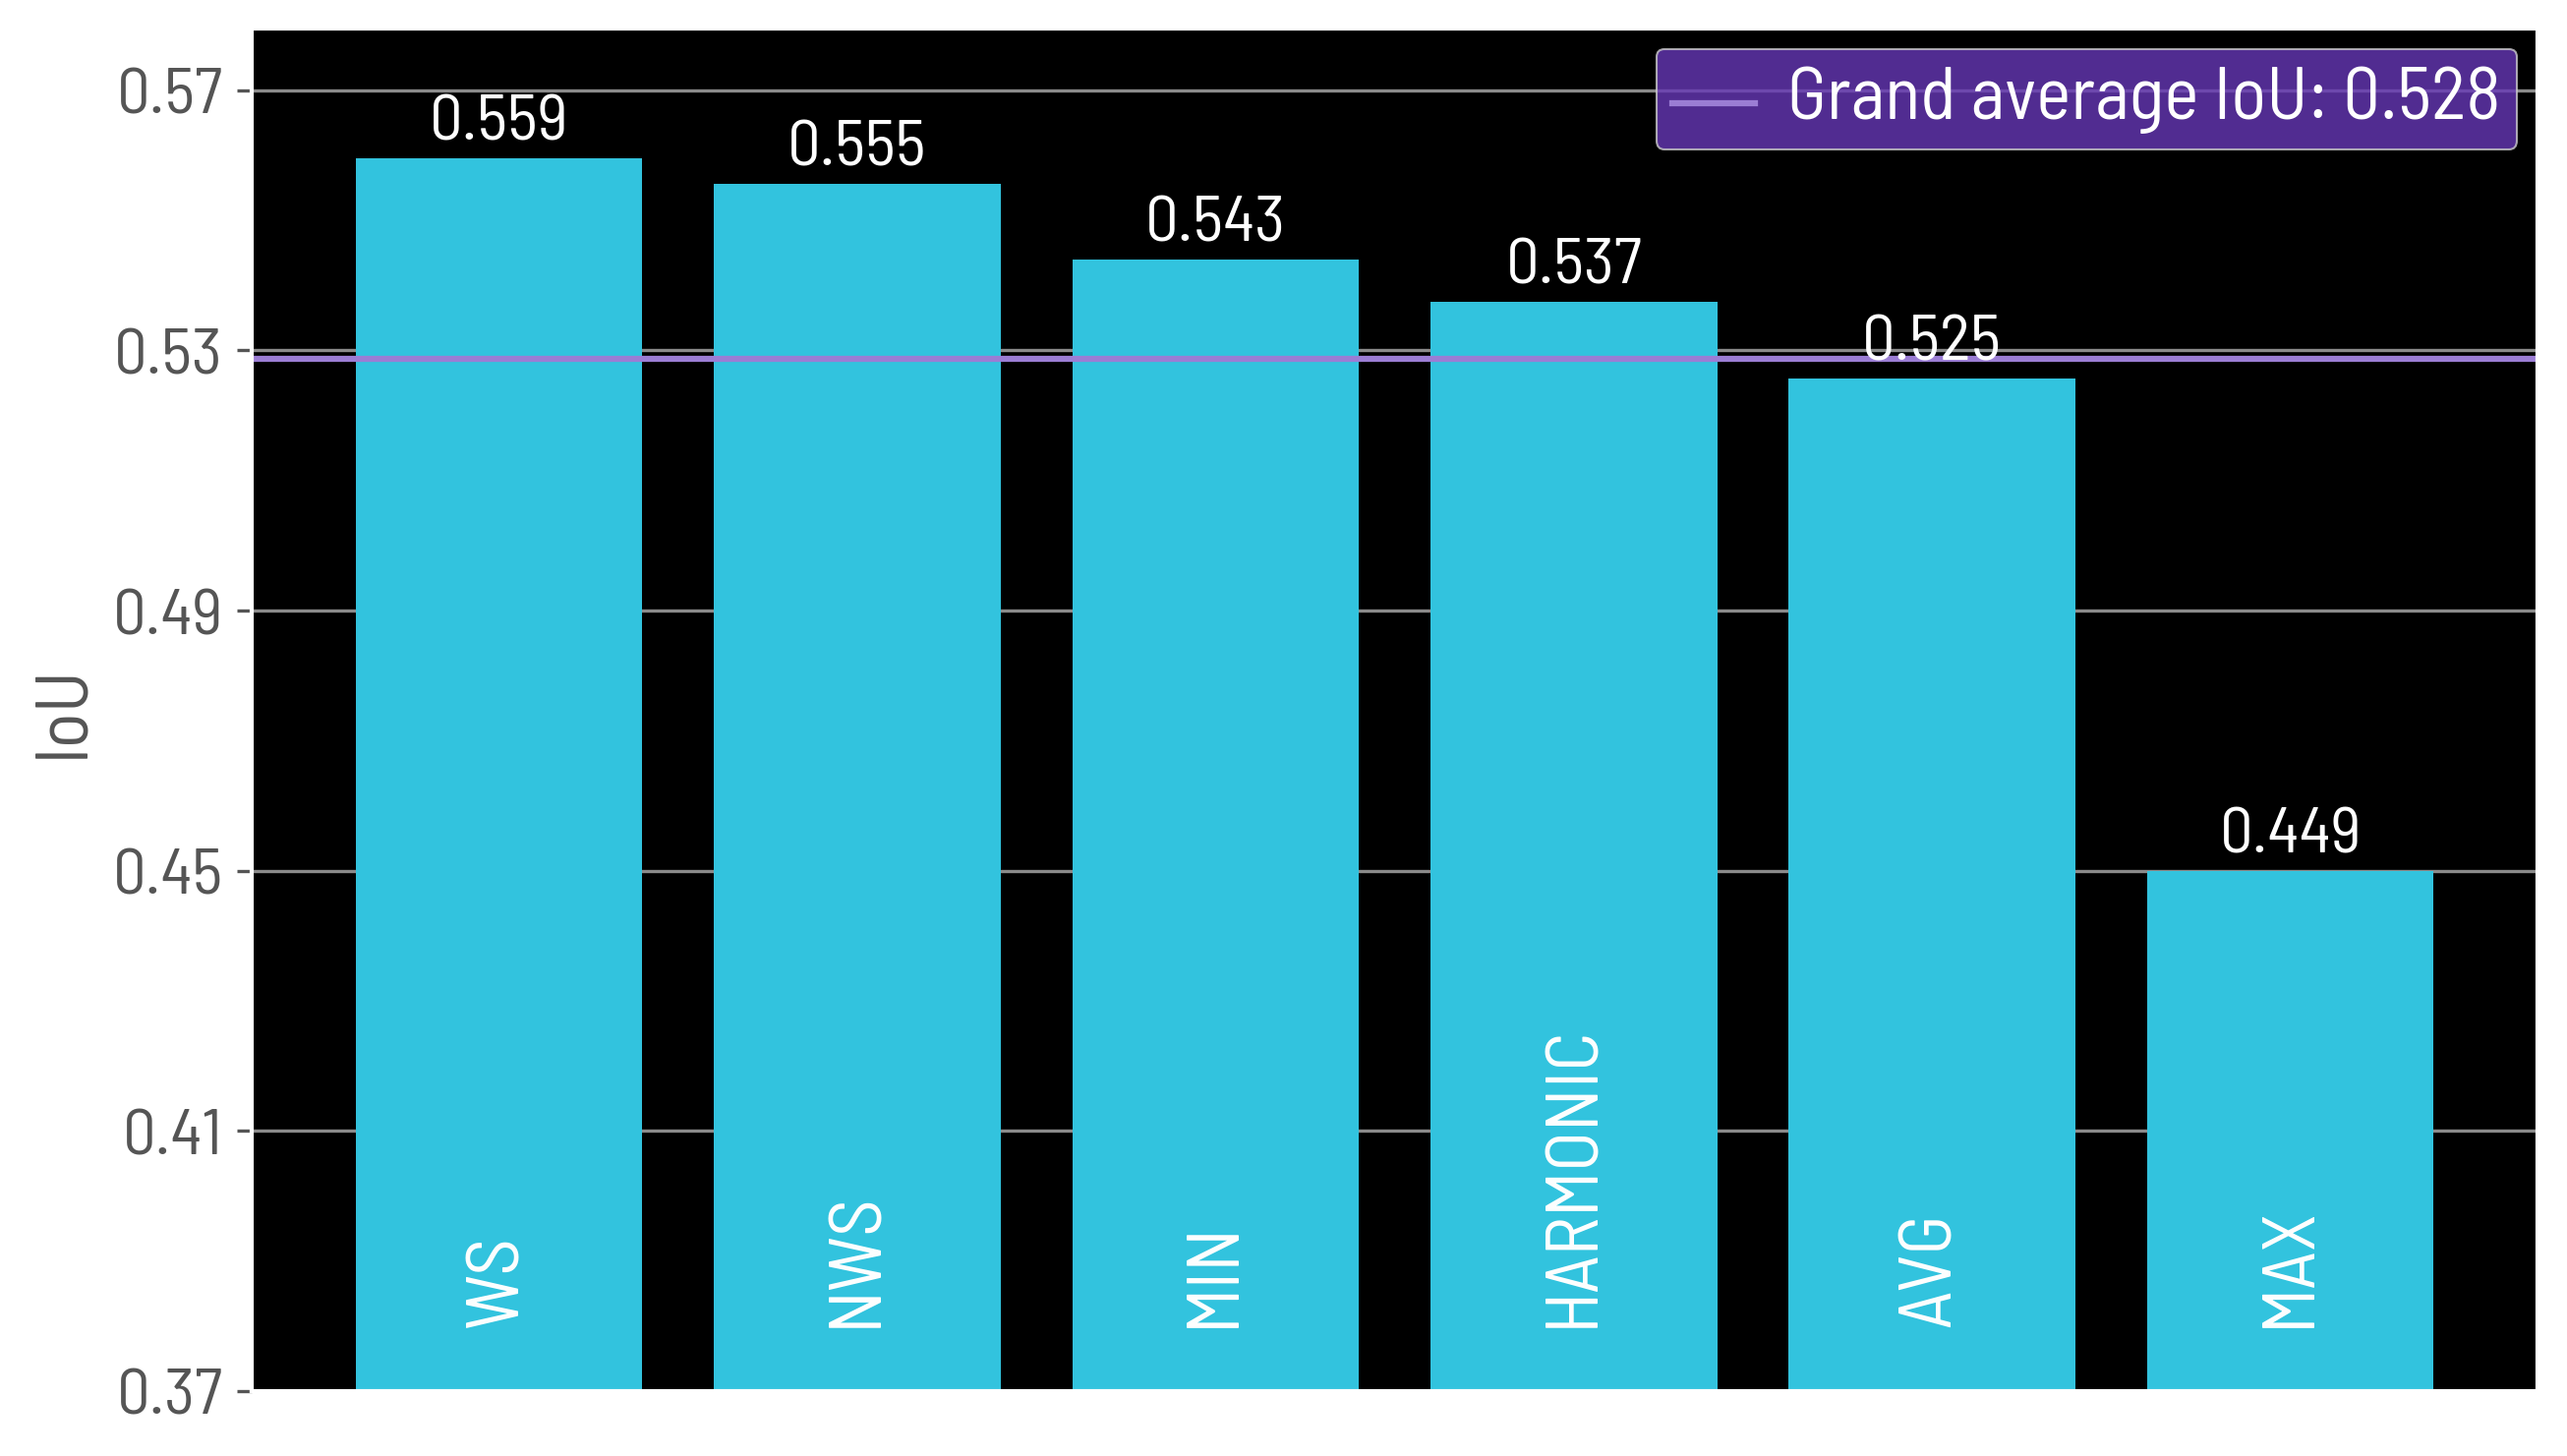
\includegraphics[width=\imgWidthcustom]{images/merge_strategy_results_melanoma_double_short_total.png}}
  \subfigure[Average IoU for Each Triple Merge Strategy]{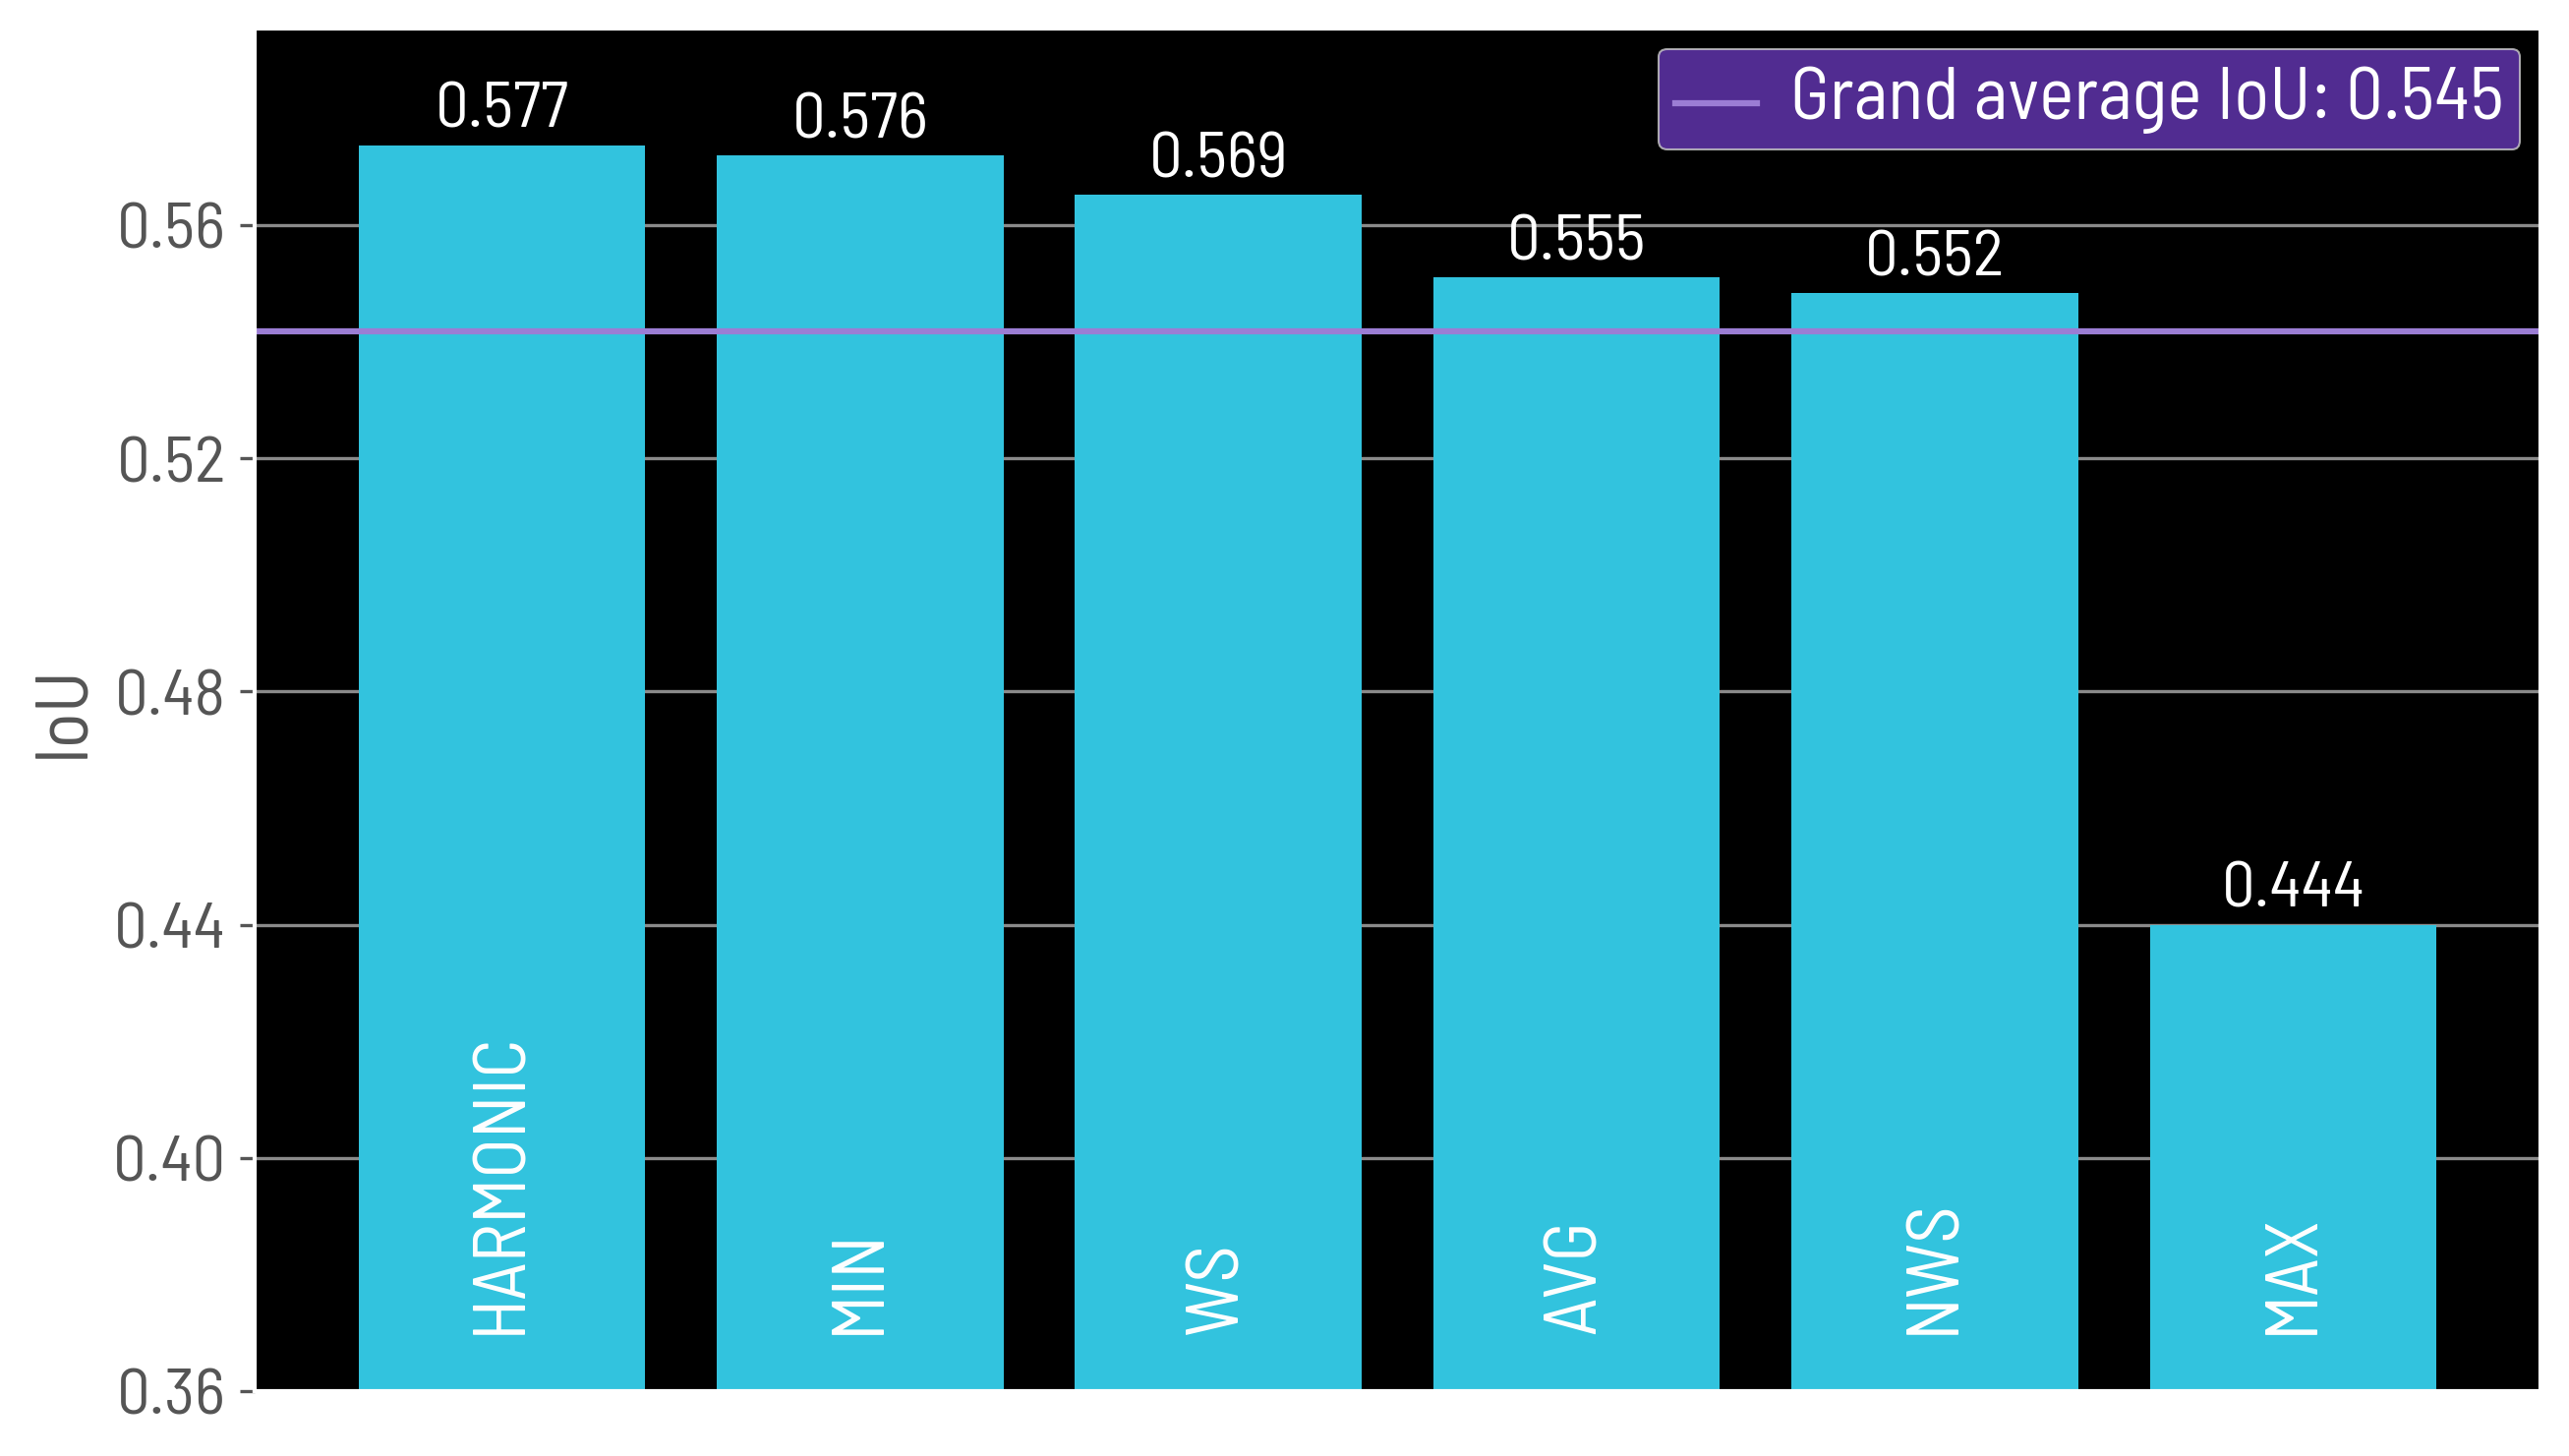
\includegraphics[width=\imgWidthcustom]{images/merge_strategy_results_melanoma_triple_short_total.png}}
  \caption[Average IoU for Each Merge Strategy (Skin Lesion)]{The figures showcase the average \ac{IoU} for each merge strategy, as well as their corresponding selection percentages, derived from an extensive set of 360 models trained on the \ac{SLD}.}
  \label{merge_strategy_results_melanoma_short}
\end{figure}
Upon examining the top-performing results in the appendix, specifically in tables \ref{tab:merge_strategy_results_melanoma_double_long} and \ref{tab:merge_strategy_results_melanoma_triple_long}, we find that no average loss combination outperforms the top baseline models summarized in table \ref{tab:baseline_skin_lesion_long}. However, there are individual exceptions. Specifically, model no. 37 and 91 from table \ref{tab:merge_strategy_results_melanoma_double_long}, as well as models no. 28 and 37 from table \ref{tab:merge_strategy_results_melanoma_double_long}, outperform the top-performing baseline model no. 1 from table \ref{tab:baseline_skin_lesion_long}.

%----------------------------------CONTINOUS PERFORMANCE (Skin Lesion)-------------------%
\subsubsection*{Continuous Performance}
\figref{continous_loss_combination_results_melanoma_short} displays the performance-based results obtained from continuous configuration no. 8. defined in table \ref{tab:final_configuration_list}. Interestingly, the two best results from the double loss combinations (a) include the \ac{HL}, which generally seemed to have been performing rather decent for this dataset. The \ac{BL} combinations performed rather low again. The triple-based loss combinations of the CE, TL, and HL displayed a decent result consisting of the average of 13 trained models with a performance close to the best baseline model average.  
\label{subsubsec:continous_melanoma}
\begin{figure}[H]%[htbp]
  \centering
  \subfigure[Average IoU for Each Double Loss Combination]{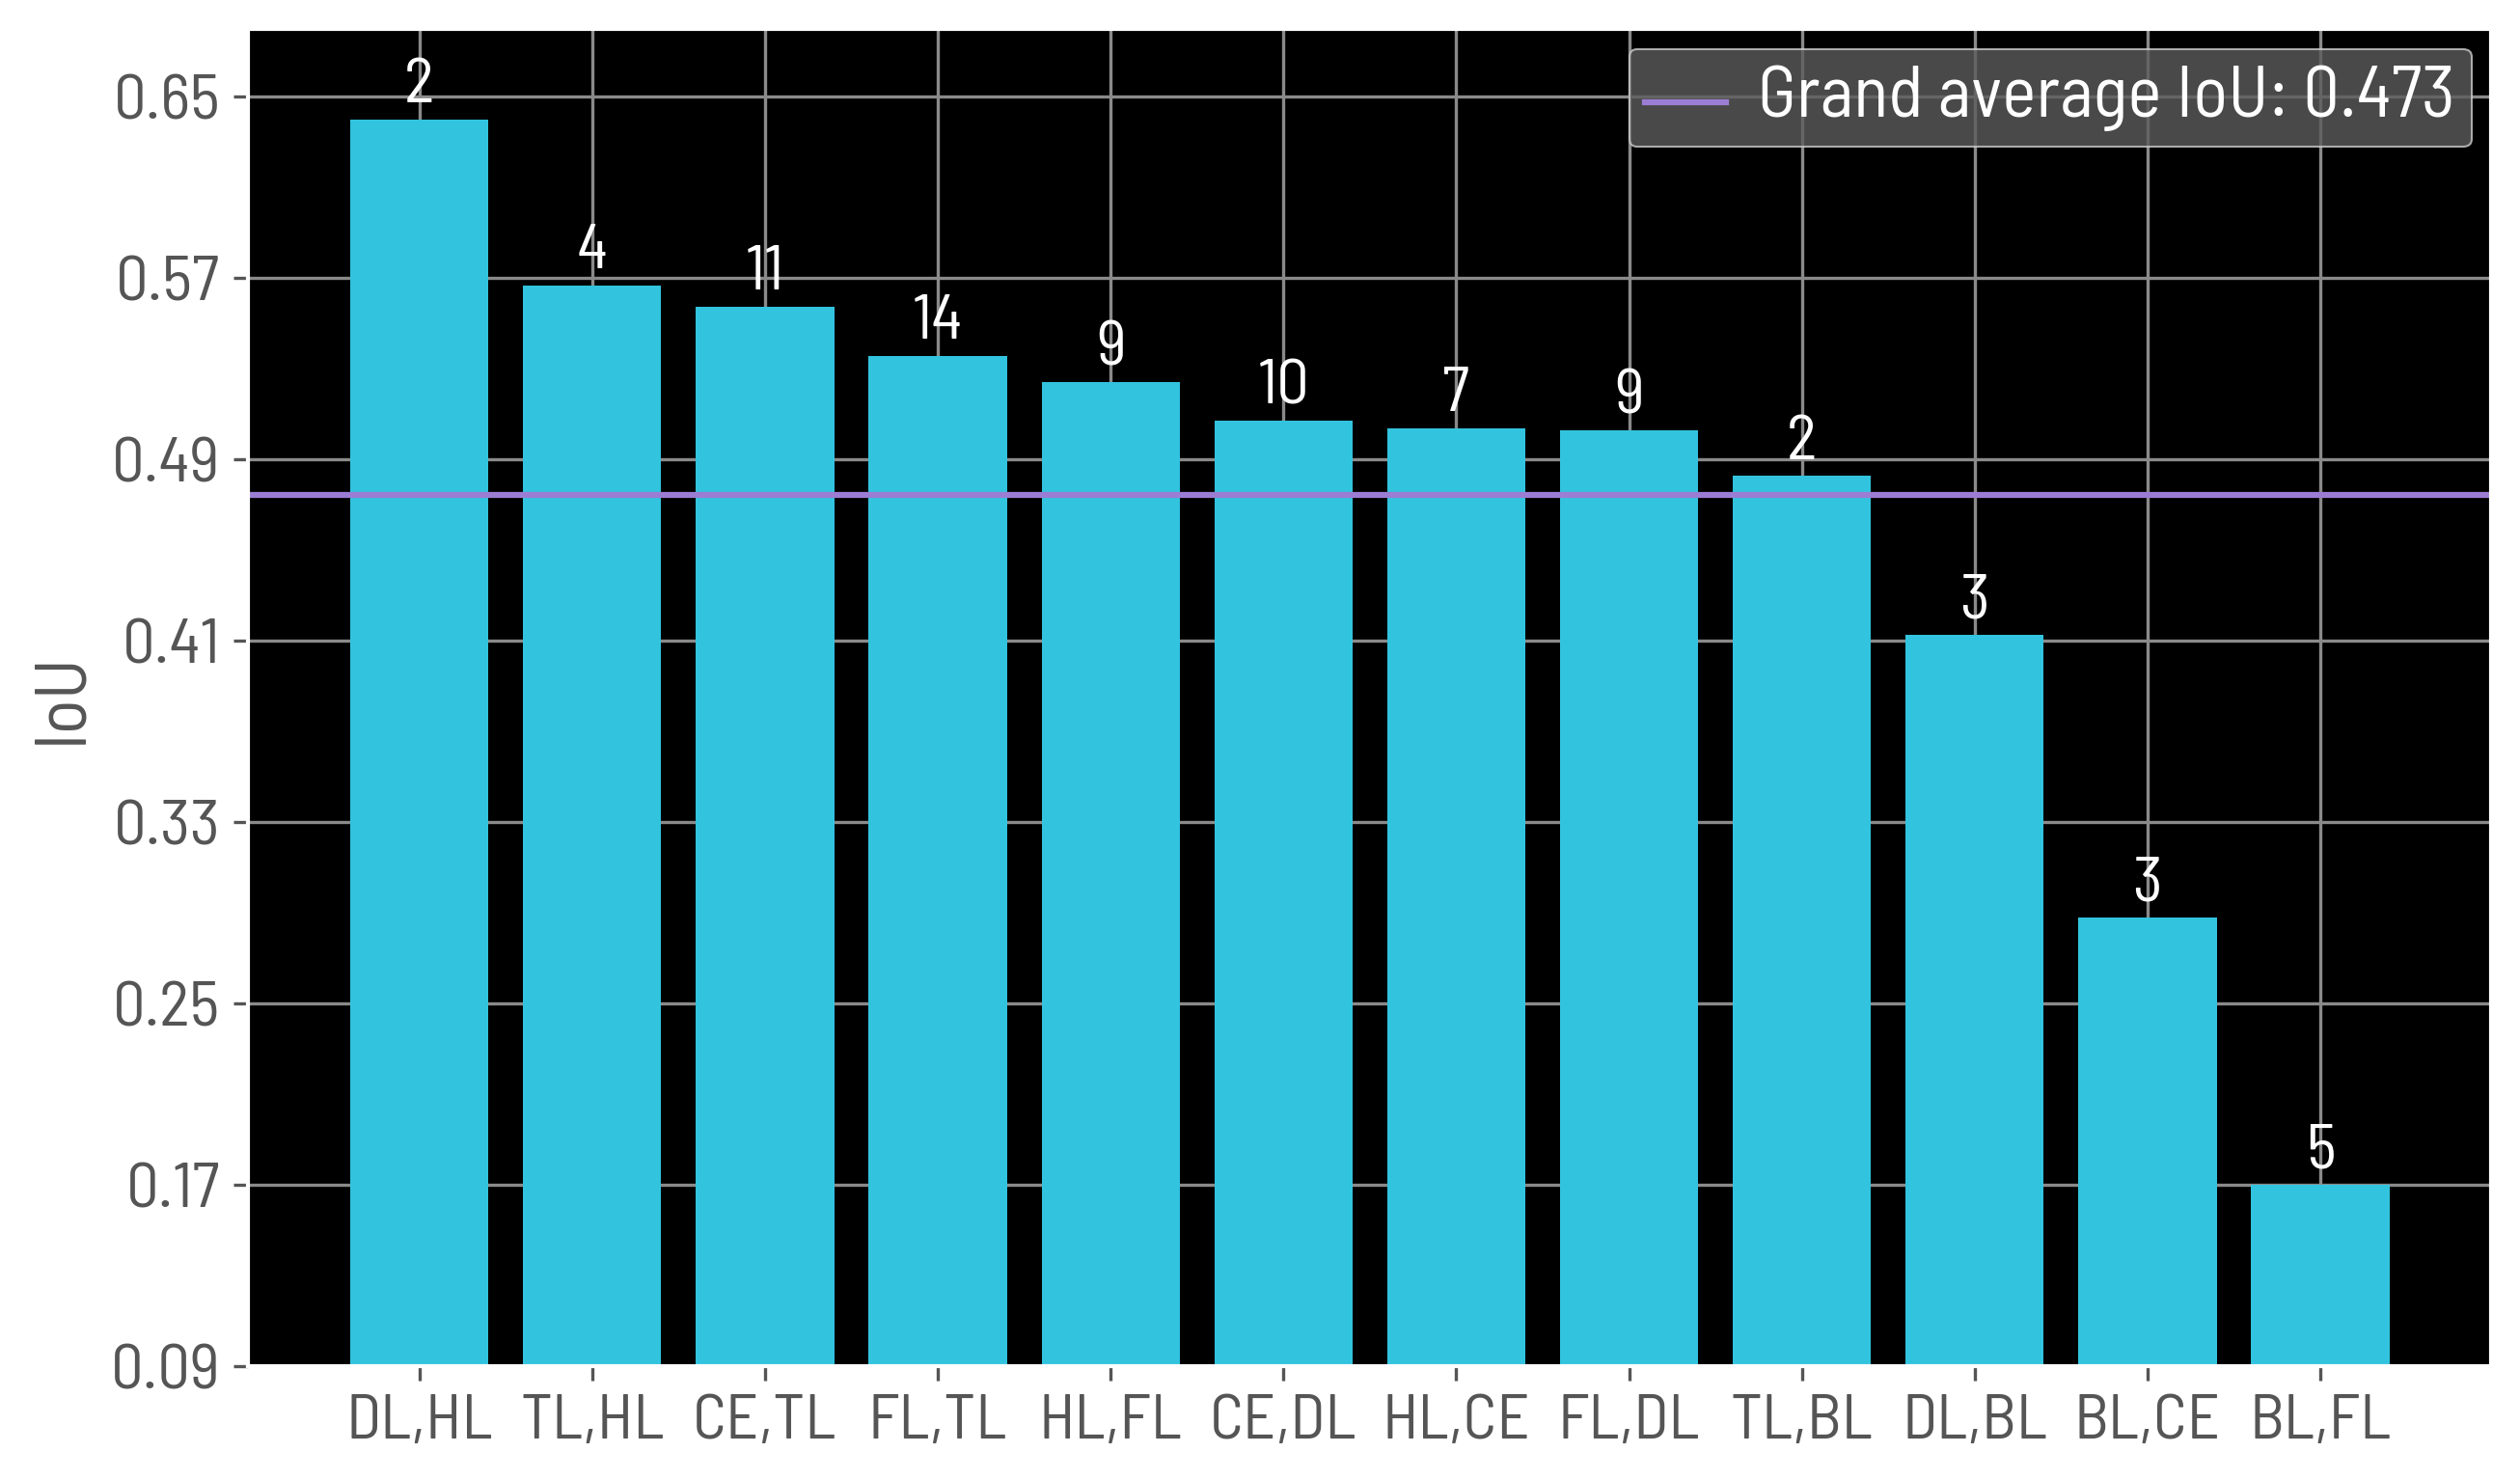
\includegraphics[width=\imgWidthcustom]{images/continous_loss_combination_results_melanoma_double_short_total.png}}
  \subfigure[Average IoU for Each Triple Loss Combination]{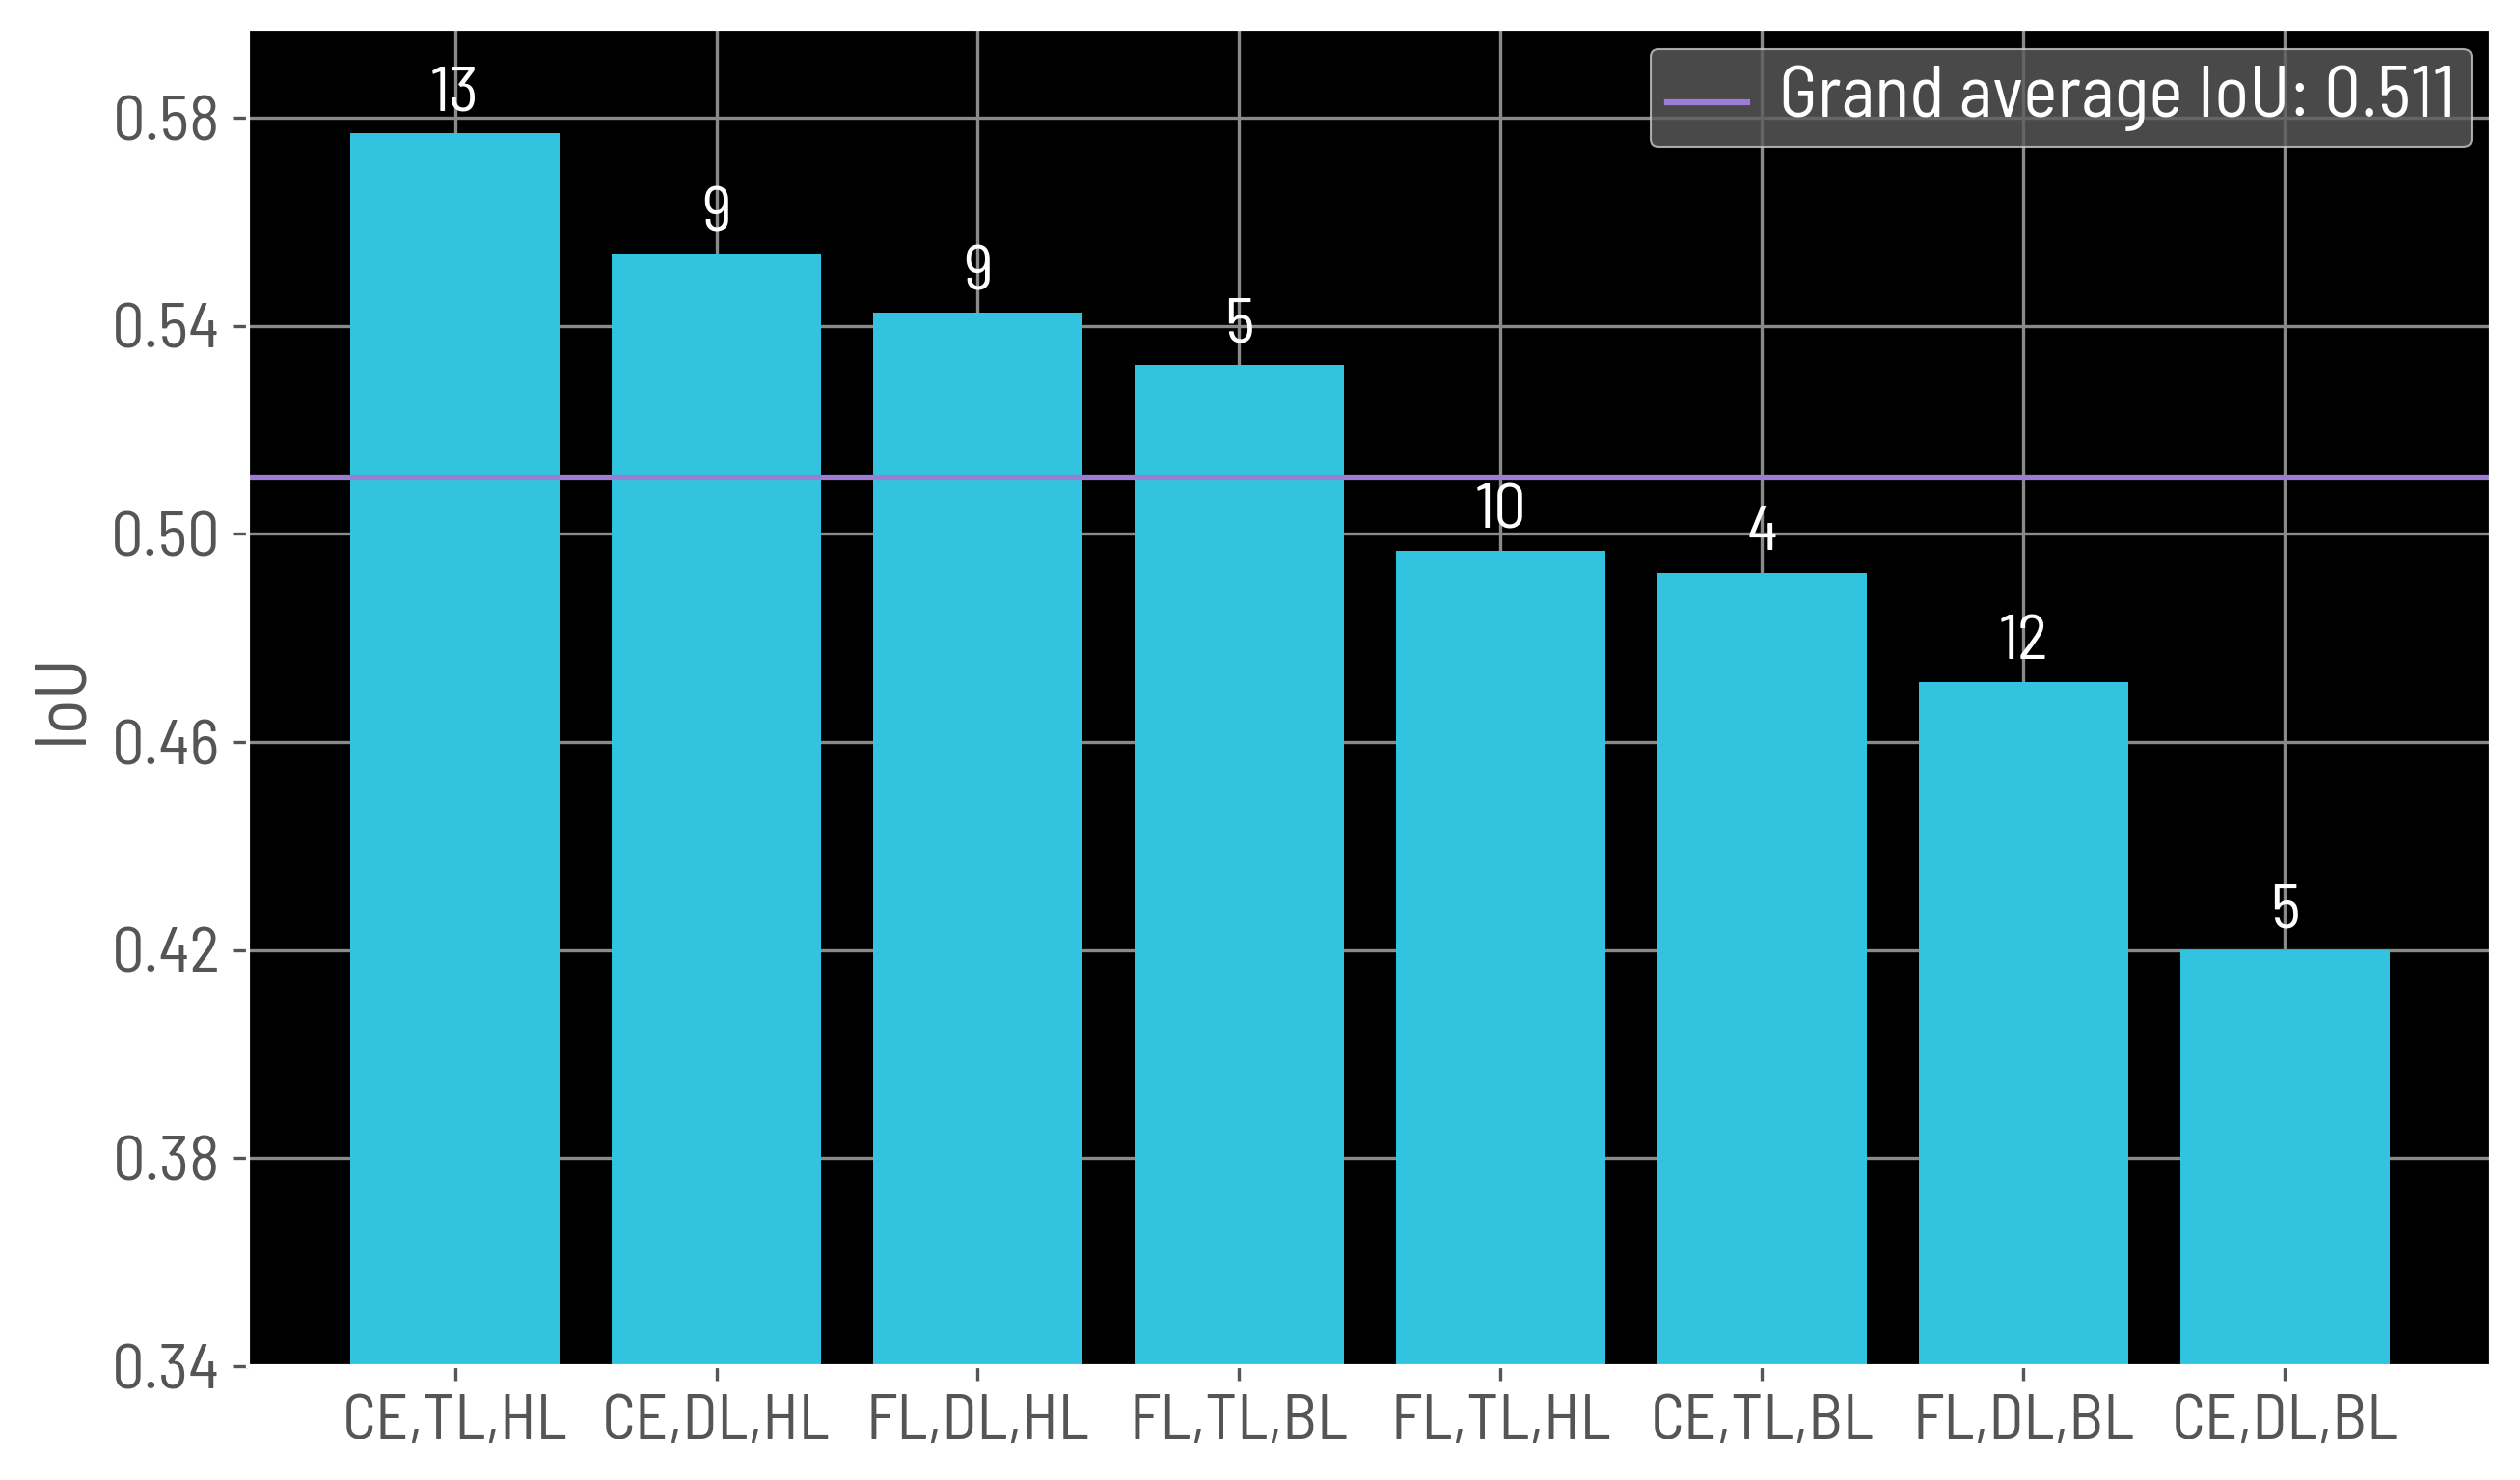
\includegraphics[width=\imgWidthcustom]{images/continous_loss_combination_results_melanoma_triple_short_total.png}}
  \caption[Average IoU for Loss Combination (Skin Lesion)]{The figures showcase the average \ac{IoU} for loss combination, derived from an extensive set of 217 models trained on the \ac{SLD} using the performance-based merge strategy.}
  \label{continous_loss_combination_results_melanoma_short}
\end{figure}
\figref{continous_results_total_melanoma} examines the two hyperparameters \texttt{pbm\_alpha} and \texttt{pbm\_I} where the graph for the former does not show a clear trend while the latter indicates that models with a higher \texttt{pbm\_I} are performing better.
\begin{figure}[H]%[htbp]
  \centering
  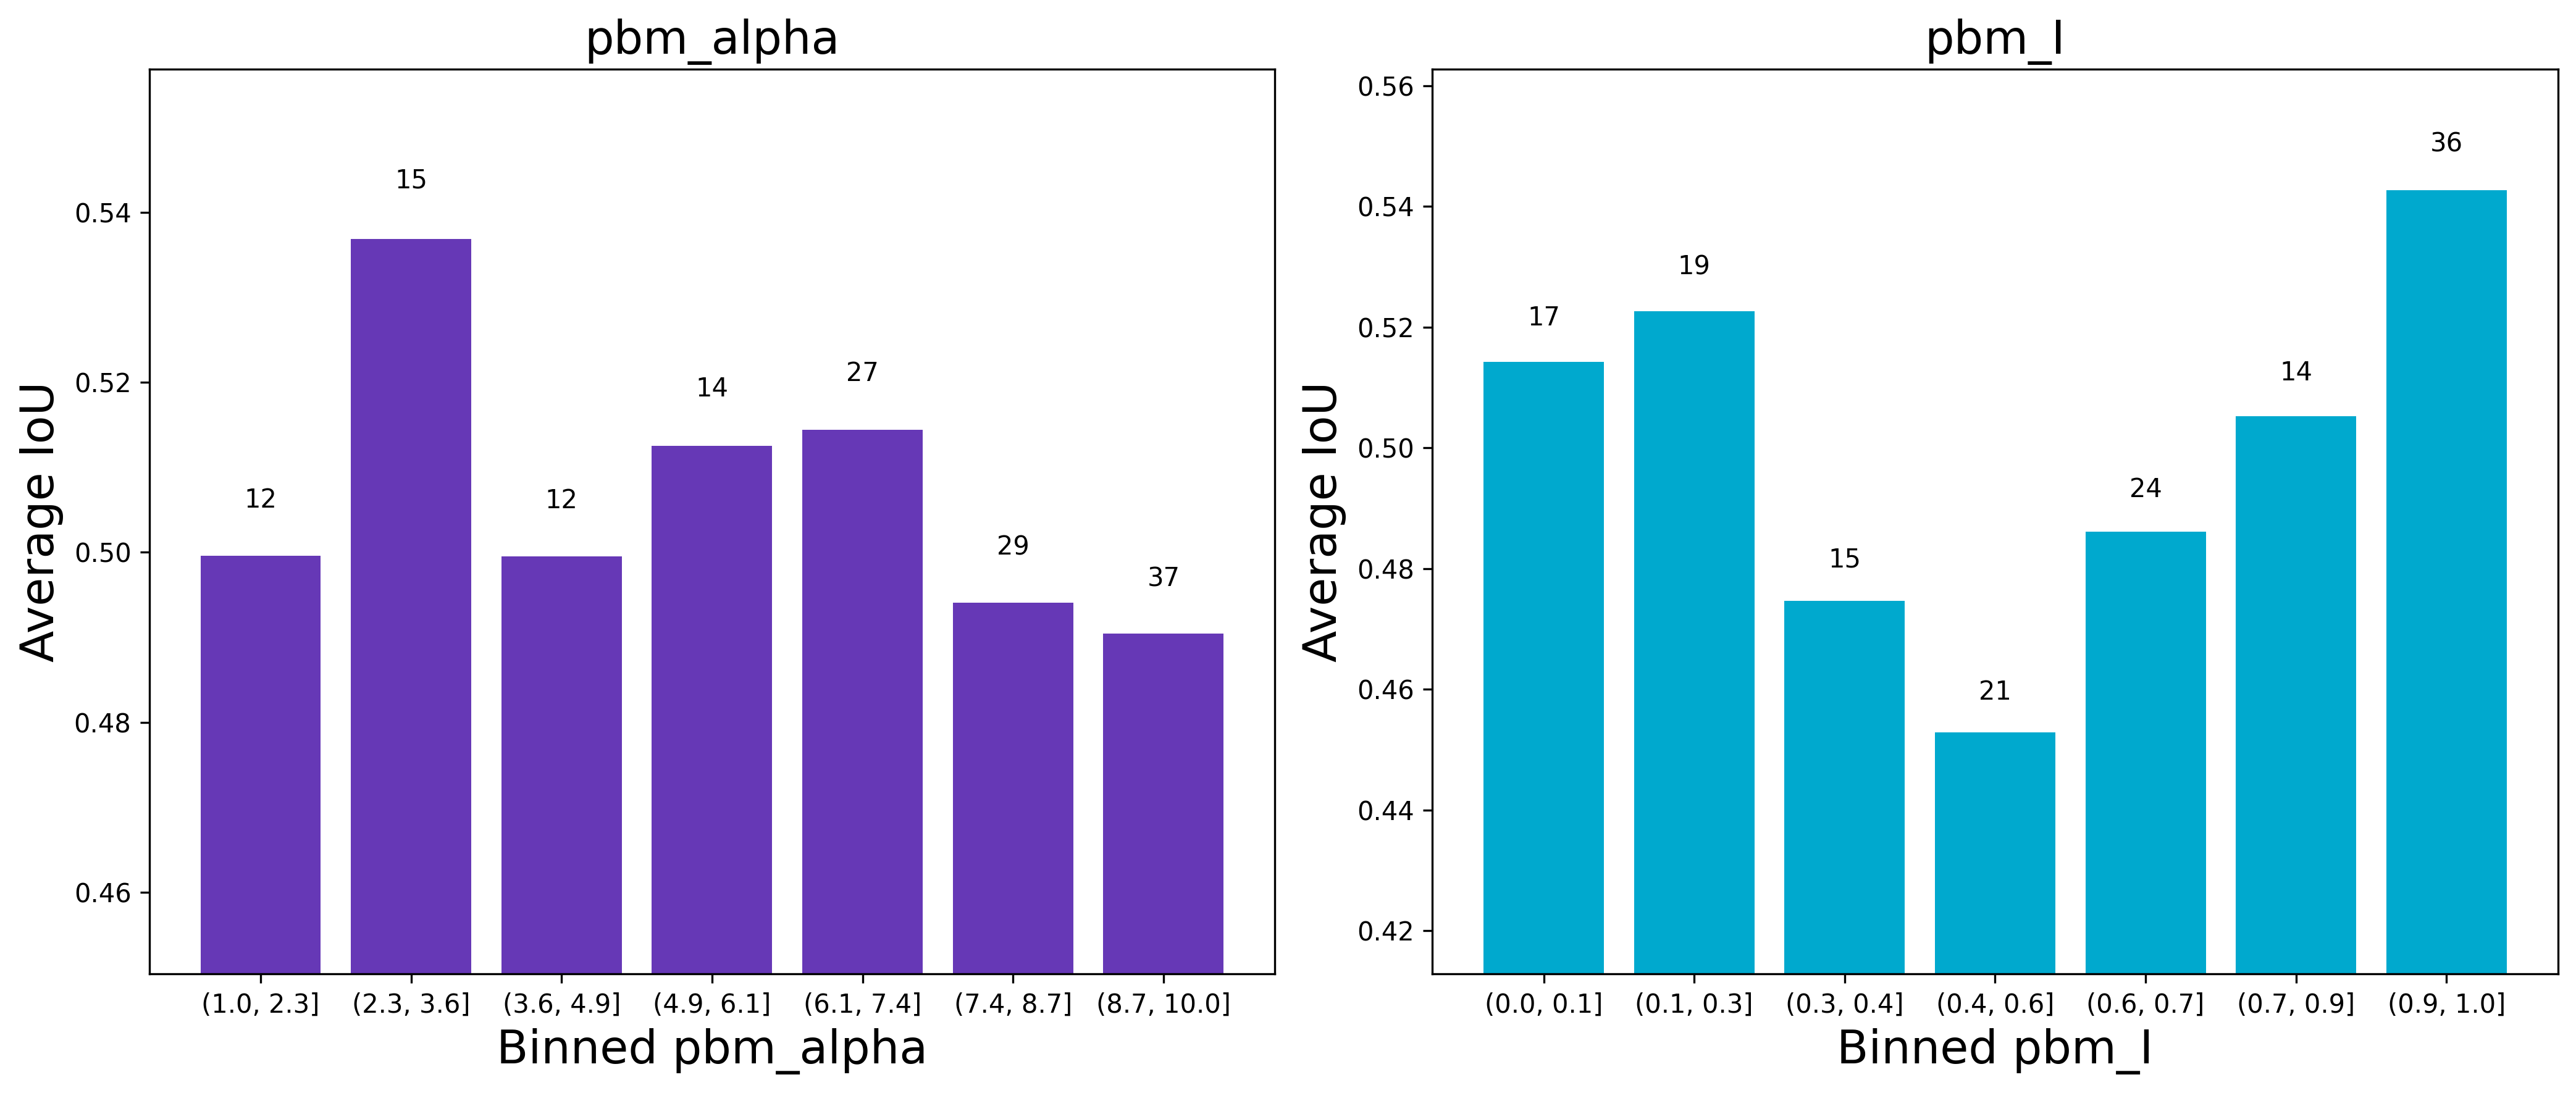
\includegraphics[width=\imgWidthL]{images/continous_hyperparameter_total_melanoma.png}
  \caption[Hyperparameter analysis]{Hyperparameter analysis for performance-based merging. The x-axis corresponds to the hyperparameter \texttt{pbm\_alpha} and \texttt{pbm\_I} defined in table \ref{tab:hyperparameters} and \secref{sec:configuration}. Both values are float with \texttt{pbm\_alpha} $\in (1,10]$ and \texttt{pbm\_I}$\in [0,1]$. The bars are labeled with the model count and represent the average \ac{IoU} for the indicated range.}
  \label{continous_results_total_melanoma}
\end{figure}

\subsubsection*{Specific Performance}
As a specific loss-merge combination for the specific configuration no.10 defined in table \ref{tab:final_configuration_list}, the NWS strategy along the combinations of \ac{CE} and \ac{TL} was used and resulted in a grand average of $0.645$ for 18 models trained, surpassing the discrete average by 3.5\% as well as the best average baseline implementation by 5.1\%. The detailed results for each model can be viewed in \secref{subsec:specific_combination_melanoma}.

%----------------------------------------------------------------------------------------%
%---------------------------------------IDRID--------------------------------------------%
%----------------------------------------------------------------------------------------%
\subsection{IDRID}
\label{subsec:idrid}
The third dataset comprises retinal images from patients with diabetic retinopathy and contains five classes, including the background. The \ac{IDRID} dataset is highly challenging due to its small size, with only 81 images, and significant class imbalance, where the background region averages 92.2\%. Furthermore, the classes are dispersed across the entire retina, adding an extra layer of difficulty for proper segmentation. As with the other datasets, the results are presented for the four configurations in table \ref{tab:final_configuration_list} (rows 11 to 14), which include the baseline, one discrete, and two continuous merge strategy configurations.

%------------------------------BASELINE PERFORMANCE (Idrid)------------------------------%
\subsubsection*{Baseline Performance}
\label{subsubsec:baseline_performance_idrid}
This subsection presents the baseline results for the \ac{IDRID}. The models for this baseline training were obtained using configuration no. 11 from the configuration table \ref{tab:final_configuration_list}. 

Configuration no. 11 was trained six times to provide a robust performance estimate. Table \ref{tab:baseline_idrid_short} displays the average results of the six models for each loss function introduced earlier. The \ac{CE} achieves the best performance, with an average \ac{IoU} of $0.341$. The grand average across all losses is 9.2\% lower at $0.249$. Note that due to the small dataset size, it was not further subdivided into smaller subsets.

\textbf{Distribution-based results}\newline
The distribution-based results with the \ac{CE} and the \ac{FL} are the top performers for this baseline training, where the \ac{CE} is even 3\% higher than the average models trained with the \ac{FL}. For both losses, it can be observed that the \ac{IoU} for the Haemorrhages and Microaneurysm classes were nearly zero. As expected, the background class displayed decent results, which can generally be neglected due to the high-class imbalance for this dataset, as illustrated in table \ref{tab:datasets}. The best meaningful results were achieved for the Optic Disc, representing the most straightforward class, followed by the Hard Exudates.

\textbf{Region-based results}\newline
The region-based loss functions performed worse on average, with up to 8.9\% less than the top model from the distribution-based results. The \ac{TL}, as expected, emphasized a higher \ac{TPR}, even if its overall performance was lower than models trained with the \ac{DL}.

\textbf{Boundary-based results}\newline
While the \ac{HL} appeared to converge, providing similar results to the region-based performance, the \ac{BL} seemed to fail, even for the background class.
% Please add the following required packages to your document preamble:
% \usepackage{graphicx}
% \usepackage[table,xcdraw]{xcolor}
% If you use beamer only pass "xcolor=table" option, i.e. \documentclass[xcolor=table]{beamer}
\begin{table}[H]
  \centering
  \resizebox{\textwidth}{!}{%
  \begin{tabular}{cc|l|c|c|c|c|c|c|c|c|c|}
  \hline
  \rowcolor[HTML]{000000} 
  \multicolumn{1}{|c|}{\cellcolor[HTML]{000000}{\color[HTML]{FFFFFF} No.}} &
    {\color[HTML]{FFFFFF} Loss type} &
    {\color[HTML]{FFFFFF} Loss} &
    {\color[HTML]{FFFFFF} Iou} &
    {\color[HTML]{FFFFFF} IoU 0} &
    {\color[HTML]{FFFFFF} IoU 1} &
    {\color[HTML]{FFFFFF} IoU 2} &
    {\color[HTML]{FFFFFF} IoU 3} &
    {\color[HTML]{FFFFFF} IoU 4} &
    {\color[HTML]{FFFFFF} PPV} &
    {\color[HTML]{FFFFFF} TPR} &
    {\color[HTML]{FFFFFF} PPV vs. TPR} \\ \hline
  \multicolumn{1}{|c|}{\textit{\textbf{1}}} &
    \cellcolor[HTML]{6638B6}{\color[HTML]{FFFFFF} \textit{\textbf{DB}}} &
    {\color[HTML]{000000} \textit{\textbf{CE}}} &
    {\color[HTML]{000000} \textit{\textbf{0.341}}} &
    {\color[HTML]{000000} \textit{\textbf{0.955}}} &
    {\color[HTML]{000000} \textit{\textbf{0.008}}} &
    {\color[HTML]{000000} \textit{\textbf{0.262}}} &
    {\color[HTML]{000000} \textit{\textbf{0.002}}} &
    {\color[HTML]{000000} \textit{\textbf{0.477}}} &
    {\color[HTML]{000000} \textit{\textbf{0.503}}} &
    {\color[HTML]{000000} \textit{\textbf{0.410}}} &
    \textit{\textbf{PPV}} \\ \hline
  \multicolumn{1}{|c|}{2} & \cellcolor[HTML]{6638B6}{\color[HTML]{FFFFFF} DB} & FL                  & 0.311 & 0.944 & 0.002 & 0.253 & 0.020 & 0.337 & 0.517 & 0.388 & PPV \\ \hline
  \multicolumn{1}{|c|}{3} & \cellcolor[HTML]{00A9CE}{\color[HTML]{FFFFFF} RB} & DL                  & 0.275 & 0.931 & 0.025 & 0.183 & 0.033 & 0.202 & 0.431 & 0.360 & PPV \\ \hline
  \multicolumn{1}{|c|}{4} & \cellcolor[HTML]{00A9CE}{\color[HTML]{FFFFFF} RB} & TL                  & 0.252 & 0.956 & 0.000 & 0.000 & 0.000 & 0.301 & 0.287 & 0.292 & TPR \\ \hline
  \multicolumn{1}{|c|}{5} & \cellcolor[HTML]{99DDFD}{\color[HTML]{FFFFFF} BB} & HL\textsubscript{1} & 0.260 & 0.944 & 0.000 & 0.000 & 0.000 & 0.354 & 0.322 & 0.309 & PPV \\ \hline
  \multicolumn{1}{|c|}{6} & \cellcolor[HTML]{99DDFD}{\color[HTML]{FFFFFF} BB} & BL                  & 0.031 & 0.131 & 0.011 & 0.006 & 0.001 & 0.006 & 0.198 & 0.166 & PPV \\ \hline
   &
     &
    \cellcolor[HTML]{000000}{\color[HTML]{FFFFFF} \textit{\textbf{Grand Average}}} &
    \cellcolor[HTML]{000000}{\color[HTML]{FFFFFF} \textit{\textbf{0.249}}} &
    \cellcolor[HTML]{000000}{\color[HTML]{FFFFFF} \textit{\textbf{0.814}}} &
    \cellcolor[HTML]{000000}{\color[HTML]{FFFFFF} \textit{\textbf{0.009}}} &
    \cellcolor[HTML]{000000}{\color[HTML]{FFFFFF} \textit{\textbf{0.128}}} &
    \cellcolor[HTML]{000000}{\color[HTML]{FFFFFF} \textit{\textbf{0.010}}} &
    \cellcolor[HTML]{000000}{\color[HTML]{FFFFFF} \textit{\textbf{0.284}}} &
    \cellcolor[HTML]{000000}{\color[HTML]{FFFFFF} \textit{\textbf{0.386}}} &
    \cellcolor[HTML]{000000}{\color[HTML]{FFFFFF} \textit{\textbf{0.326}}} &
    \cellcolor[HTML]{000000}{\color[HTML]{FFFFFF} \textit{\textbf{PPV}}} \\ \cline{3-12} 
  \end{tabular}%
  }
  \caption[Overall baseline results for the IDRID]{The table presents a summary of the average values of various metrics for six baseline models corresponding trained for each loss function. The total number of models trained for this baseline result is 36. The columns $IoU_0,\hdots,IoU_4$ represent the five classes, Background, Haemorrhages, Hard Exudates, Microaneurys and Optic Disc. The column titled \squote{PPV vs. TPR}" illustrates the trade-off between a high \acf{PPV} and low \acf{TPR}, or vice versa, for each model.}
  \label{tab:baseline_idrid_short}
  \end{table}

%----------------------------------OVERALL PERFORMANCE (Idrid)---------------------------%
\subsubsection*{Overall Performance}
\label{subsubsec:idrid_overall_performance}
The following two heatmaps represent the average performance for every loss and merge strategy combination of the models obtained from configuration no. 12 and configuration no. 13 presented in \ref{tab:final_configuration_list}. Configuration no. 12 consists of a model count of $120\:\text{models} = 6\:\text{merge strategies} \times20\:\text{loss combinations}$. Even if the best practice could not be observed by training this configuration six times equally as the baseline, the configuration was trained two times to provide a more robust average with just a single run resulting in a total of 240 models from configuration no. 12. The heatmap additionally consists of the continuous configuration no. 13 with an additional model count of 430. Configuration no. 13 requires a search through a continuous hyperparameter space, so the model count is not set beforehand.

While the exact average for each loss combination and merge strategy is discussed in subsequent chapters, the heatmap already provides some valuable intuition about suitable or unsuitable combinations for this dataset. The average top-performing loss/merge combination for the double combo achieves a substantial increase of 4.9 \% in terms of \ac{IoU} compared to the top-performing baseline models. It can also be seen that some loss combinations or merge strategies fail to provide meaningful results, such as the MIN strategy or the TL, HL loss combination. 
\begin{figure}[H]%[htbp]
  \centering
  \subfigure[Overall performance of double combinations]{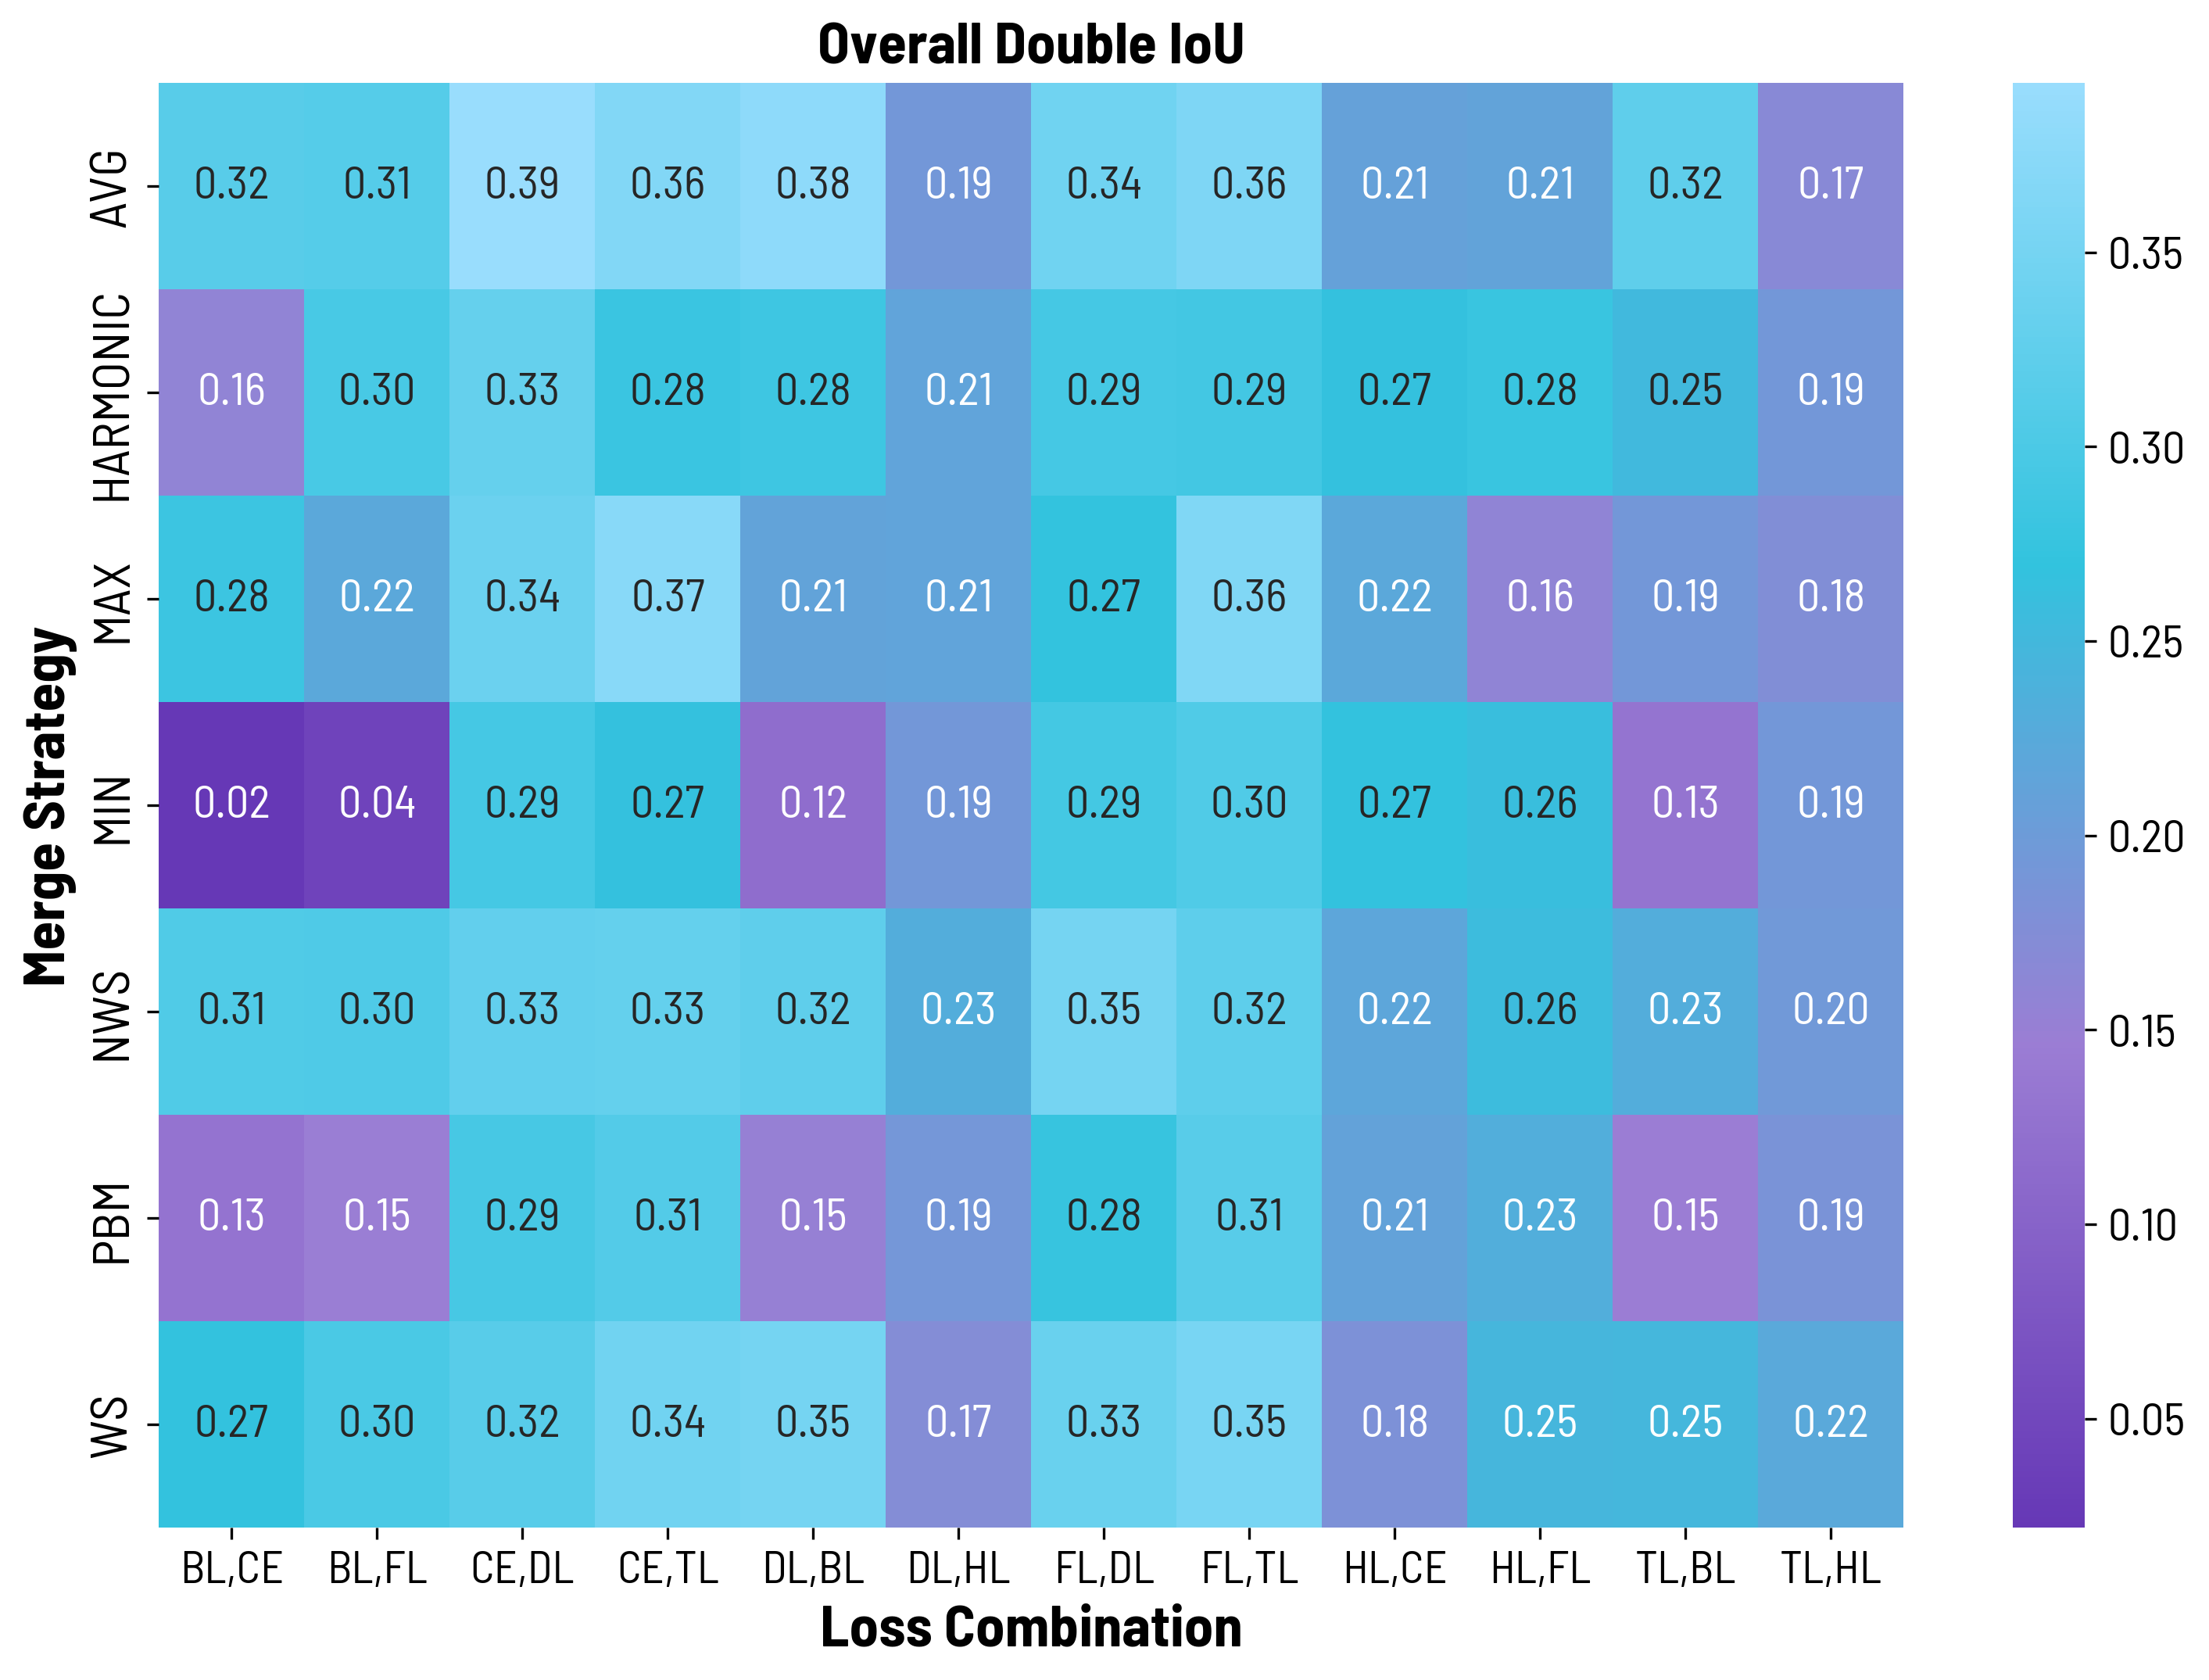
\includegraphics[width=\imgWidthcustom]{images/overall_results_double_idrid.png}}
  \subfigure[Overall performance of triple combinations]{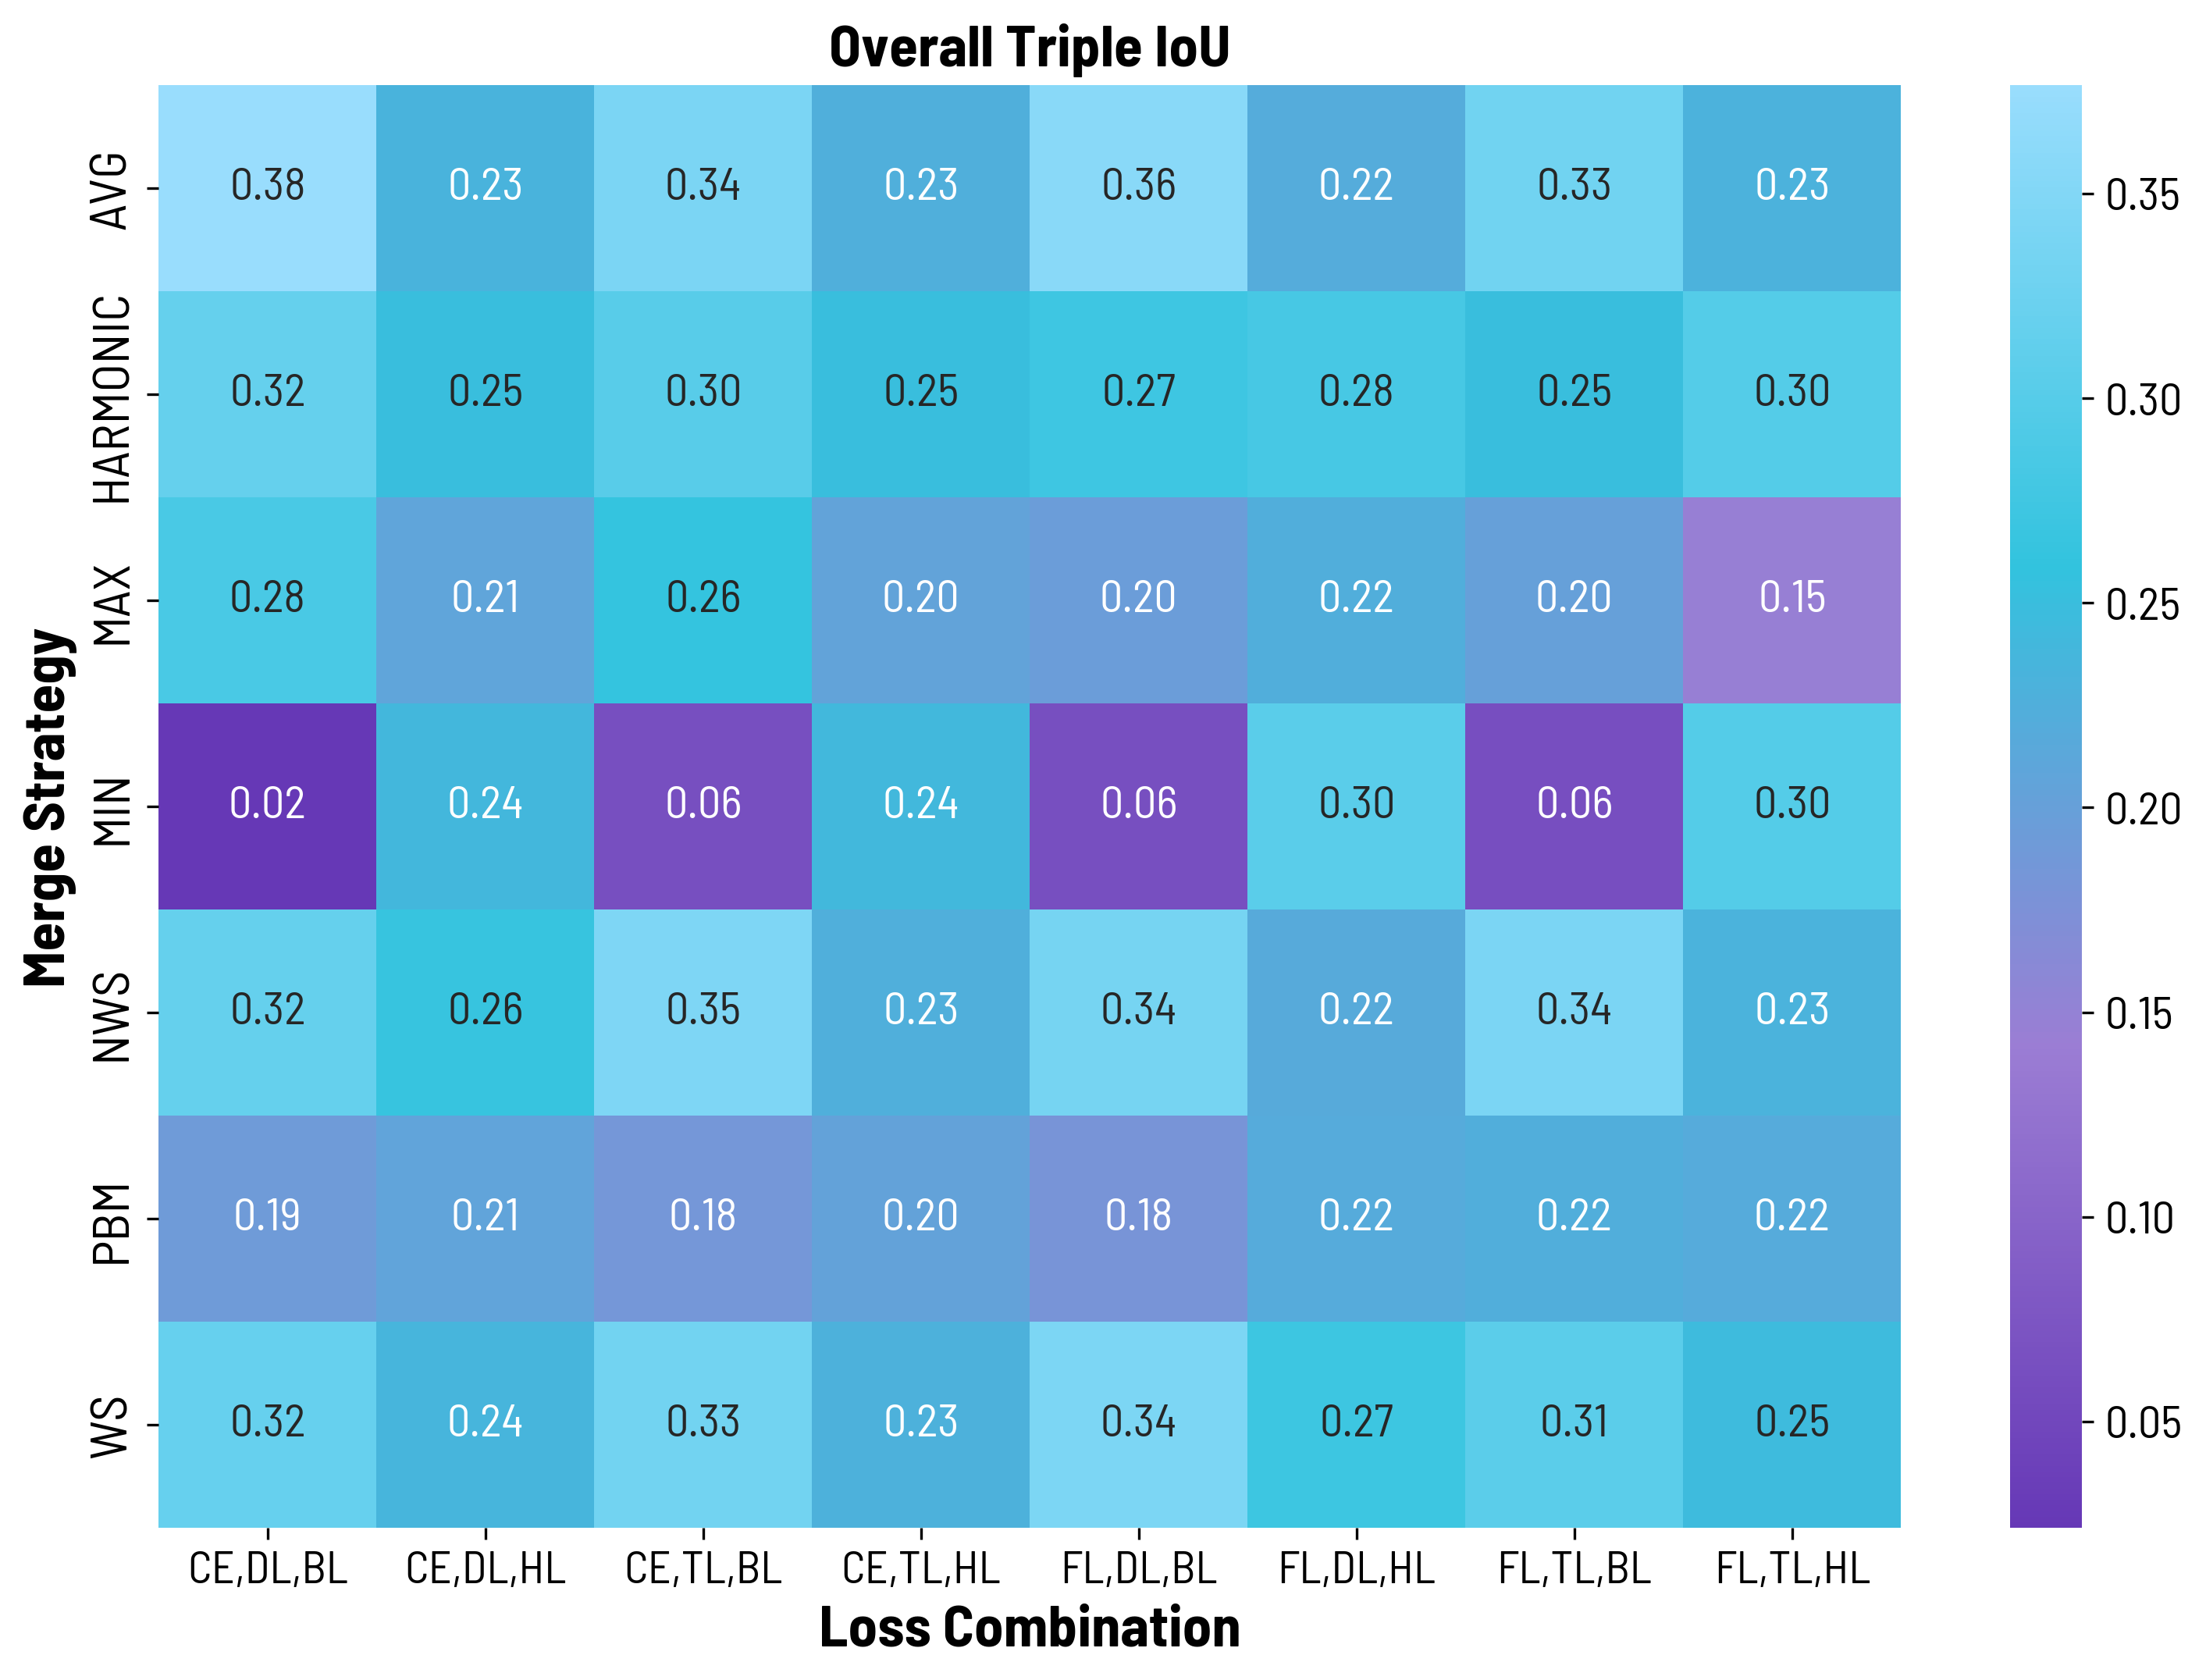
\includegraphics[width=\imgWidthcustom]{images/overall_results_triple_idrid.png}}
  \caption[Overall performance of triple combinations]{Average \ac{IoU} for all double and triple loss-merge combinations.}
  \label{overall_double_triple_idrid}
\end{figure}

A noticeable similarity comparing heatmap (a) from \ref{overall_double_triple_idrid} with heatmap (b) from \ref{overall_double_triple_idrid} is that the MIN and PBM strategies performed very low in both results. \figref{min_strategy_idrid_hd_ce} illustrates an example where a generally low-performing loss with small values gets selected exclusively as the high-performing loss initiates with larger values.
\begin{figure}[H]%[htbp]
  \centering
  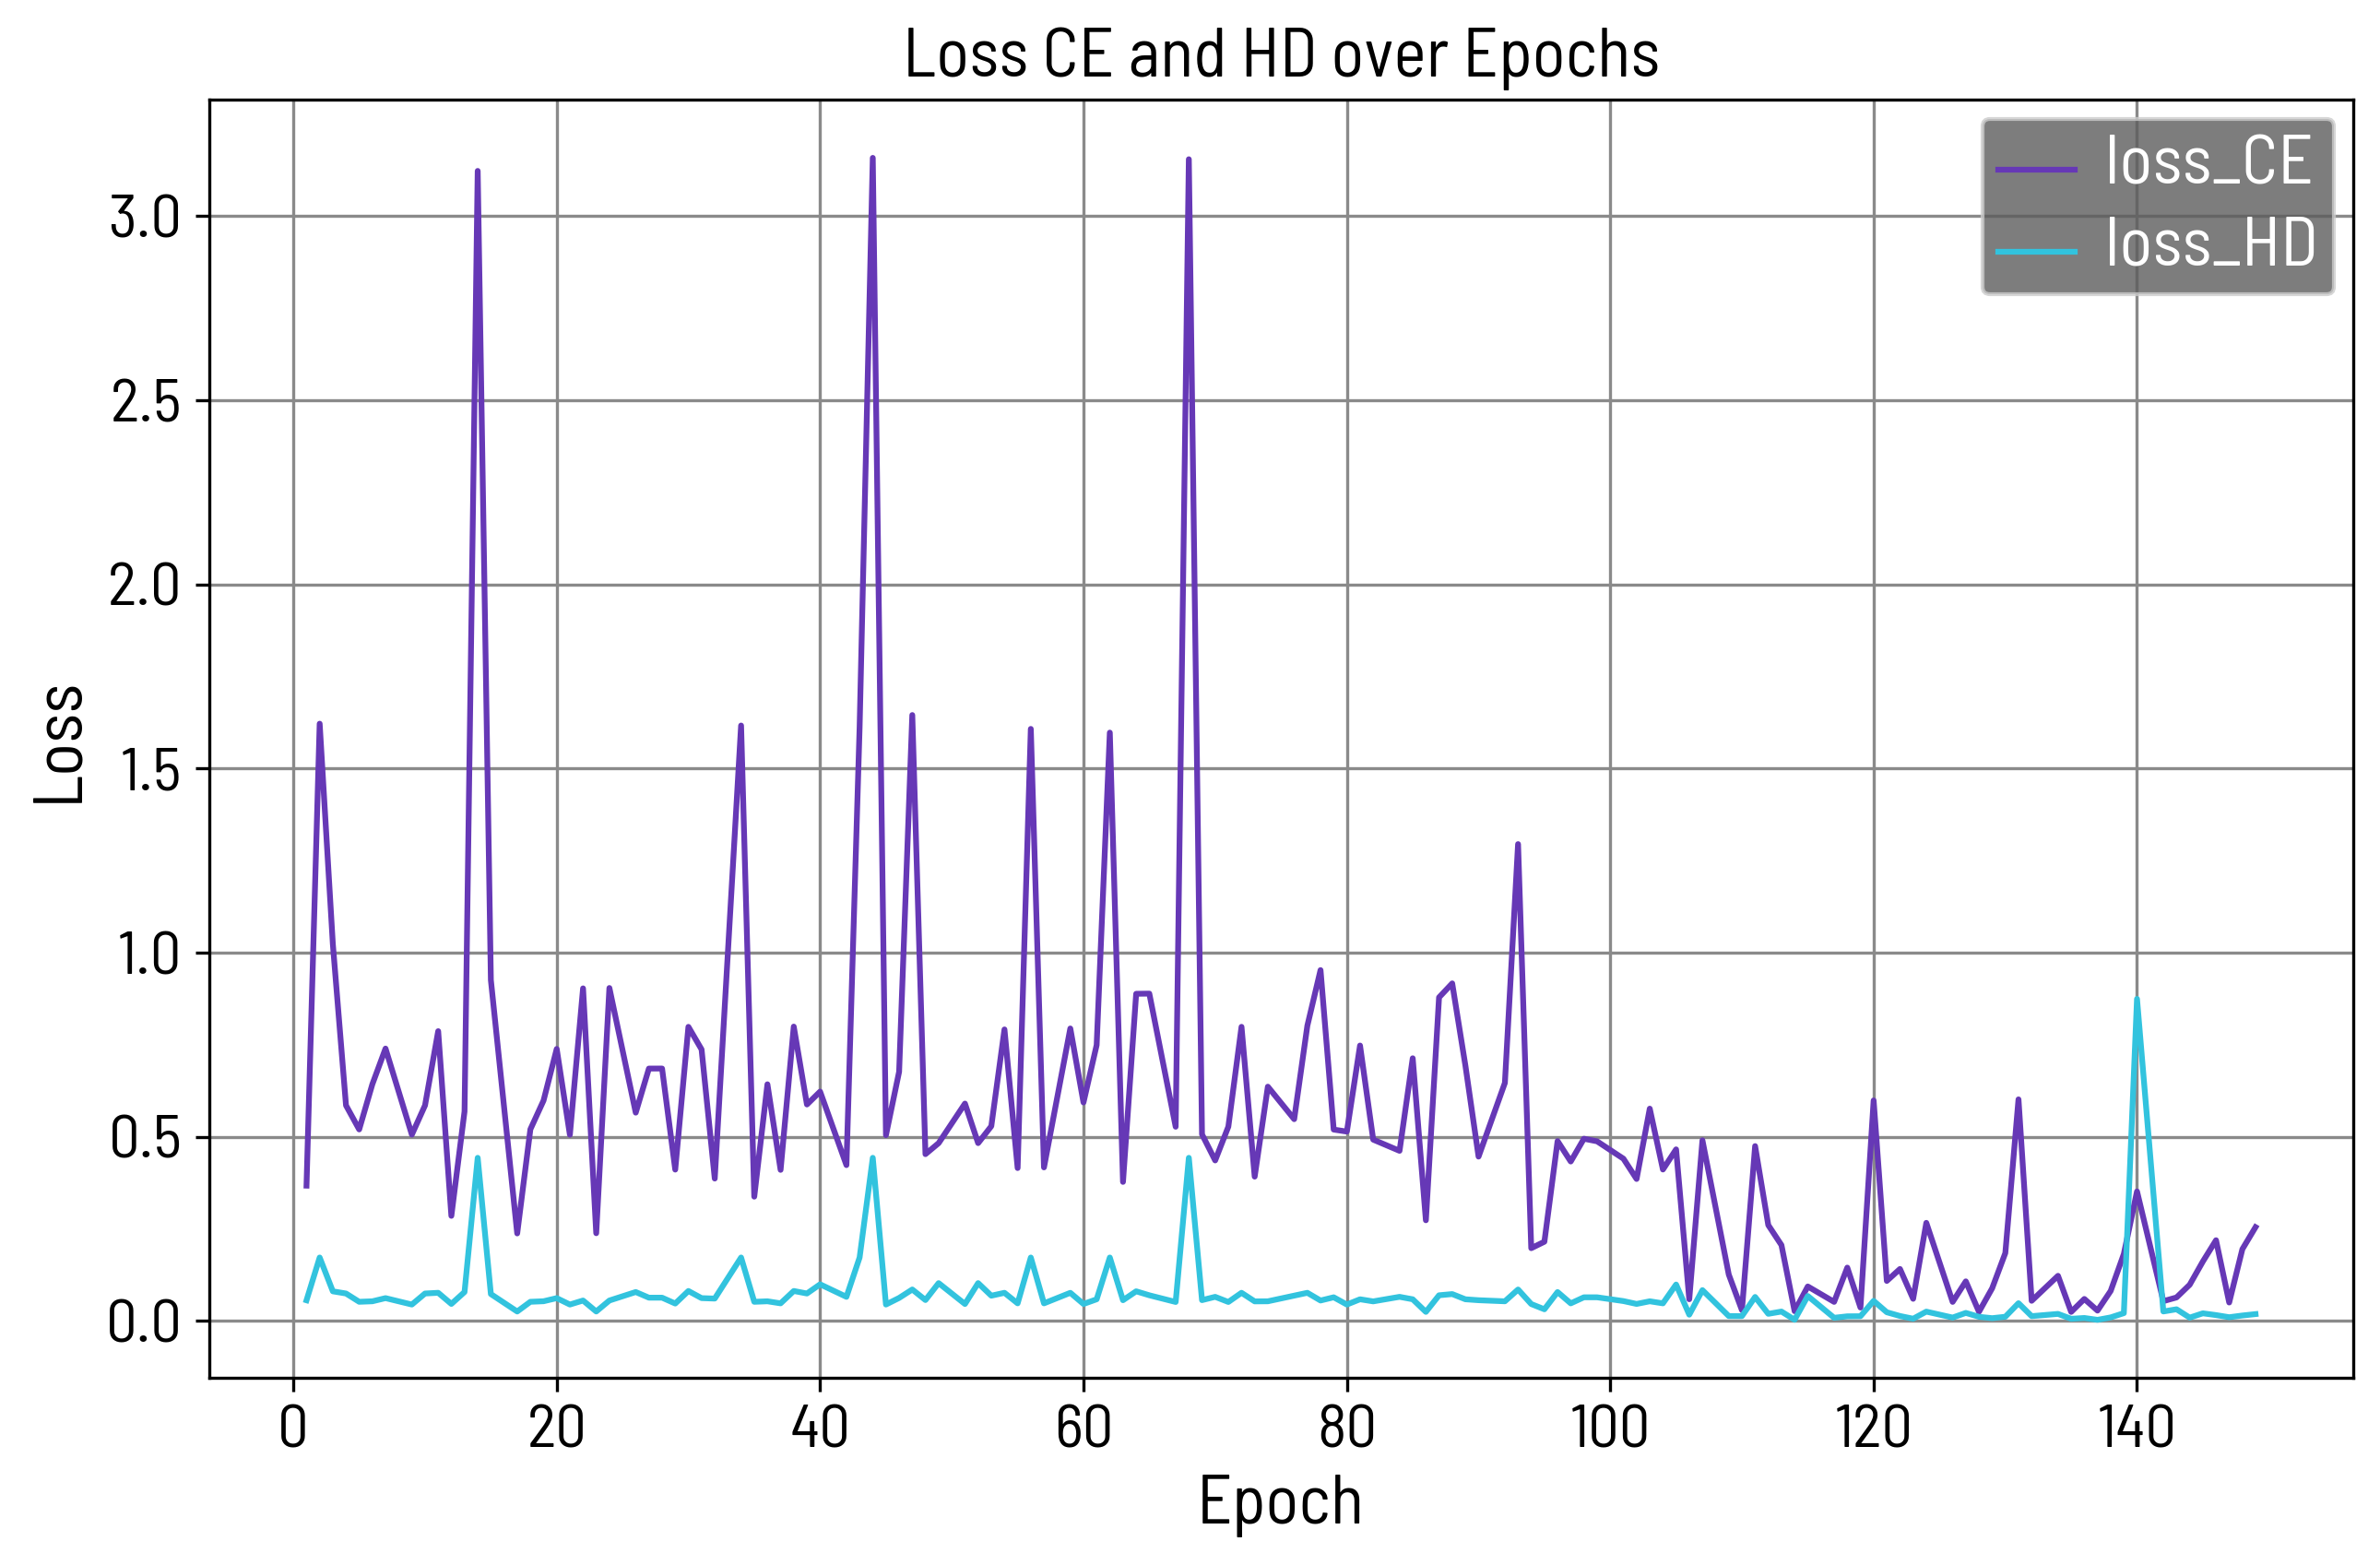
\includegraphics[width=\imgWidthM]{images/min_strategy_idrid_hd_ce.png}
  \caption[MIN strategy learning curves]{Learning curves for a model trained with a \ac{HL}\ac{CE} combination using the MIN strategy. It can be seen that the strategy always selects the \ac{HL} as feedback for gradient descent, completely ignoring the \ac{CE} due to its higher initial values.}
  \label{min_strategy_idrid_hd_ce}
\end{figure}
The following section provides a detailed result for every loss combination and merge strategy.

%----------------------------------DISCRETE PERFORMANCE (Idrid)--------------------------%
\subsubsection*{Discrete Performance}
This section exclusively presents the models obtained from configuration no. 12 presented in table \ref{tab:final_configuration_list}. The configuration is named discrete as it does not require an extensive search of hyperparameters and consists of a fixed number of models for every configuration run. The following results are presented from the loss combination and merge strategy perspective, illustrated as bar plots sorted by the best-performing averages.

\textbf{Loss combination results}\newline
\figref{discrete_loss_combination_results_idrid_short} illustrates the average performance for all 240 models created from training configuration no. 12, by double and triple loss combinations. The height of each bar represents the average results in terms of \ac{IoU} corresponding to the average of the respective column of the double or triple heatmap presented earlier. 

For the double loss combinations, it can be immediately seen that the average results obtained from using distribution and region-based loss combinations outperformed any combination containing a boundary-based loss function. The top four loss combination averages lay above an \ac{IoU} of $0.3$, close to the best-performing baseline averages. Looking at the \ref{tab:loss_combination_results_idrid_double_long}, which lists the top performing results from double loss combinations for the \ac{IDRID}, we see that the CE, TL average, is 3.1\% higher than the average of the top three baseline models represented by model no. 1 to 3 from table \ref{tab:baseline_idrid_long}.

The triple loss combinations resulted in a lower performance indicating that boundary-based loss functions could not improve the performance compared to double loss combinations. Comparing the top three performing models (No. 13,14,15) from table \ref{tab:loss_combination_results_idrid_triple_long} to the baseline top three results from the baseline, we can observe an increase of 2.2 \%.

\begin{figure}[H]%[htbp]
  \centering
  \subfigure[Average IoU for Each Double Loss Combination]{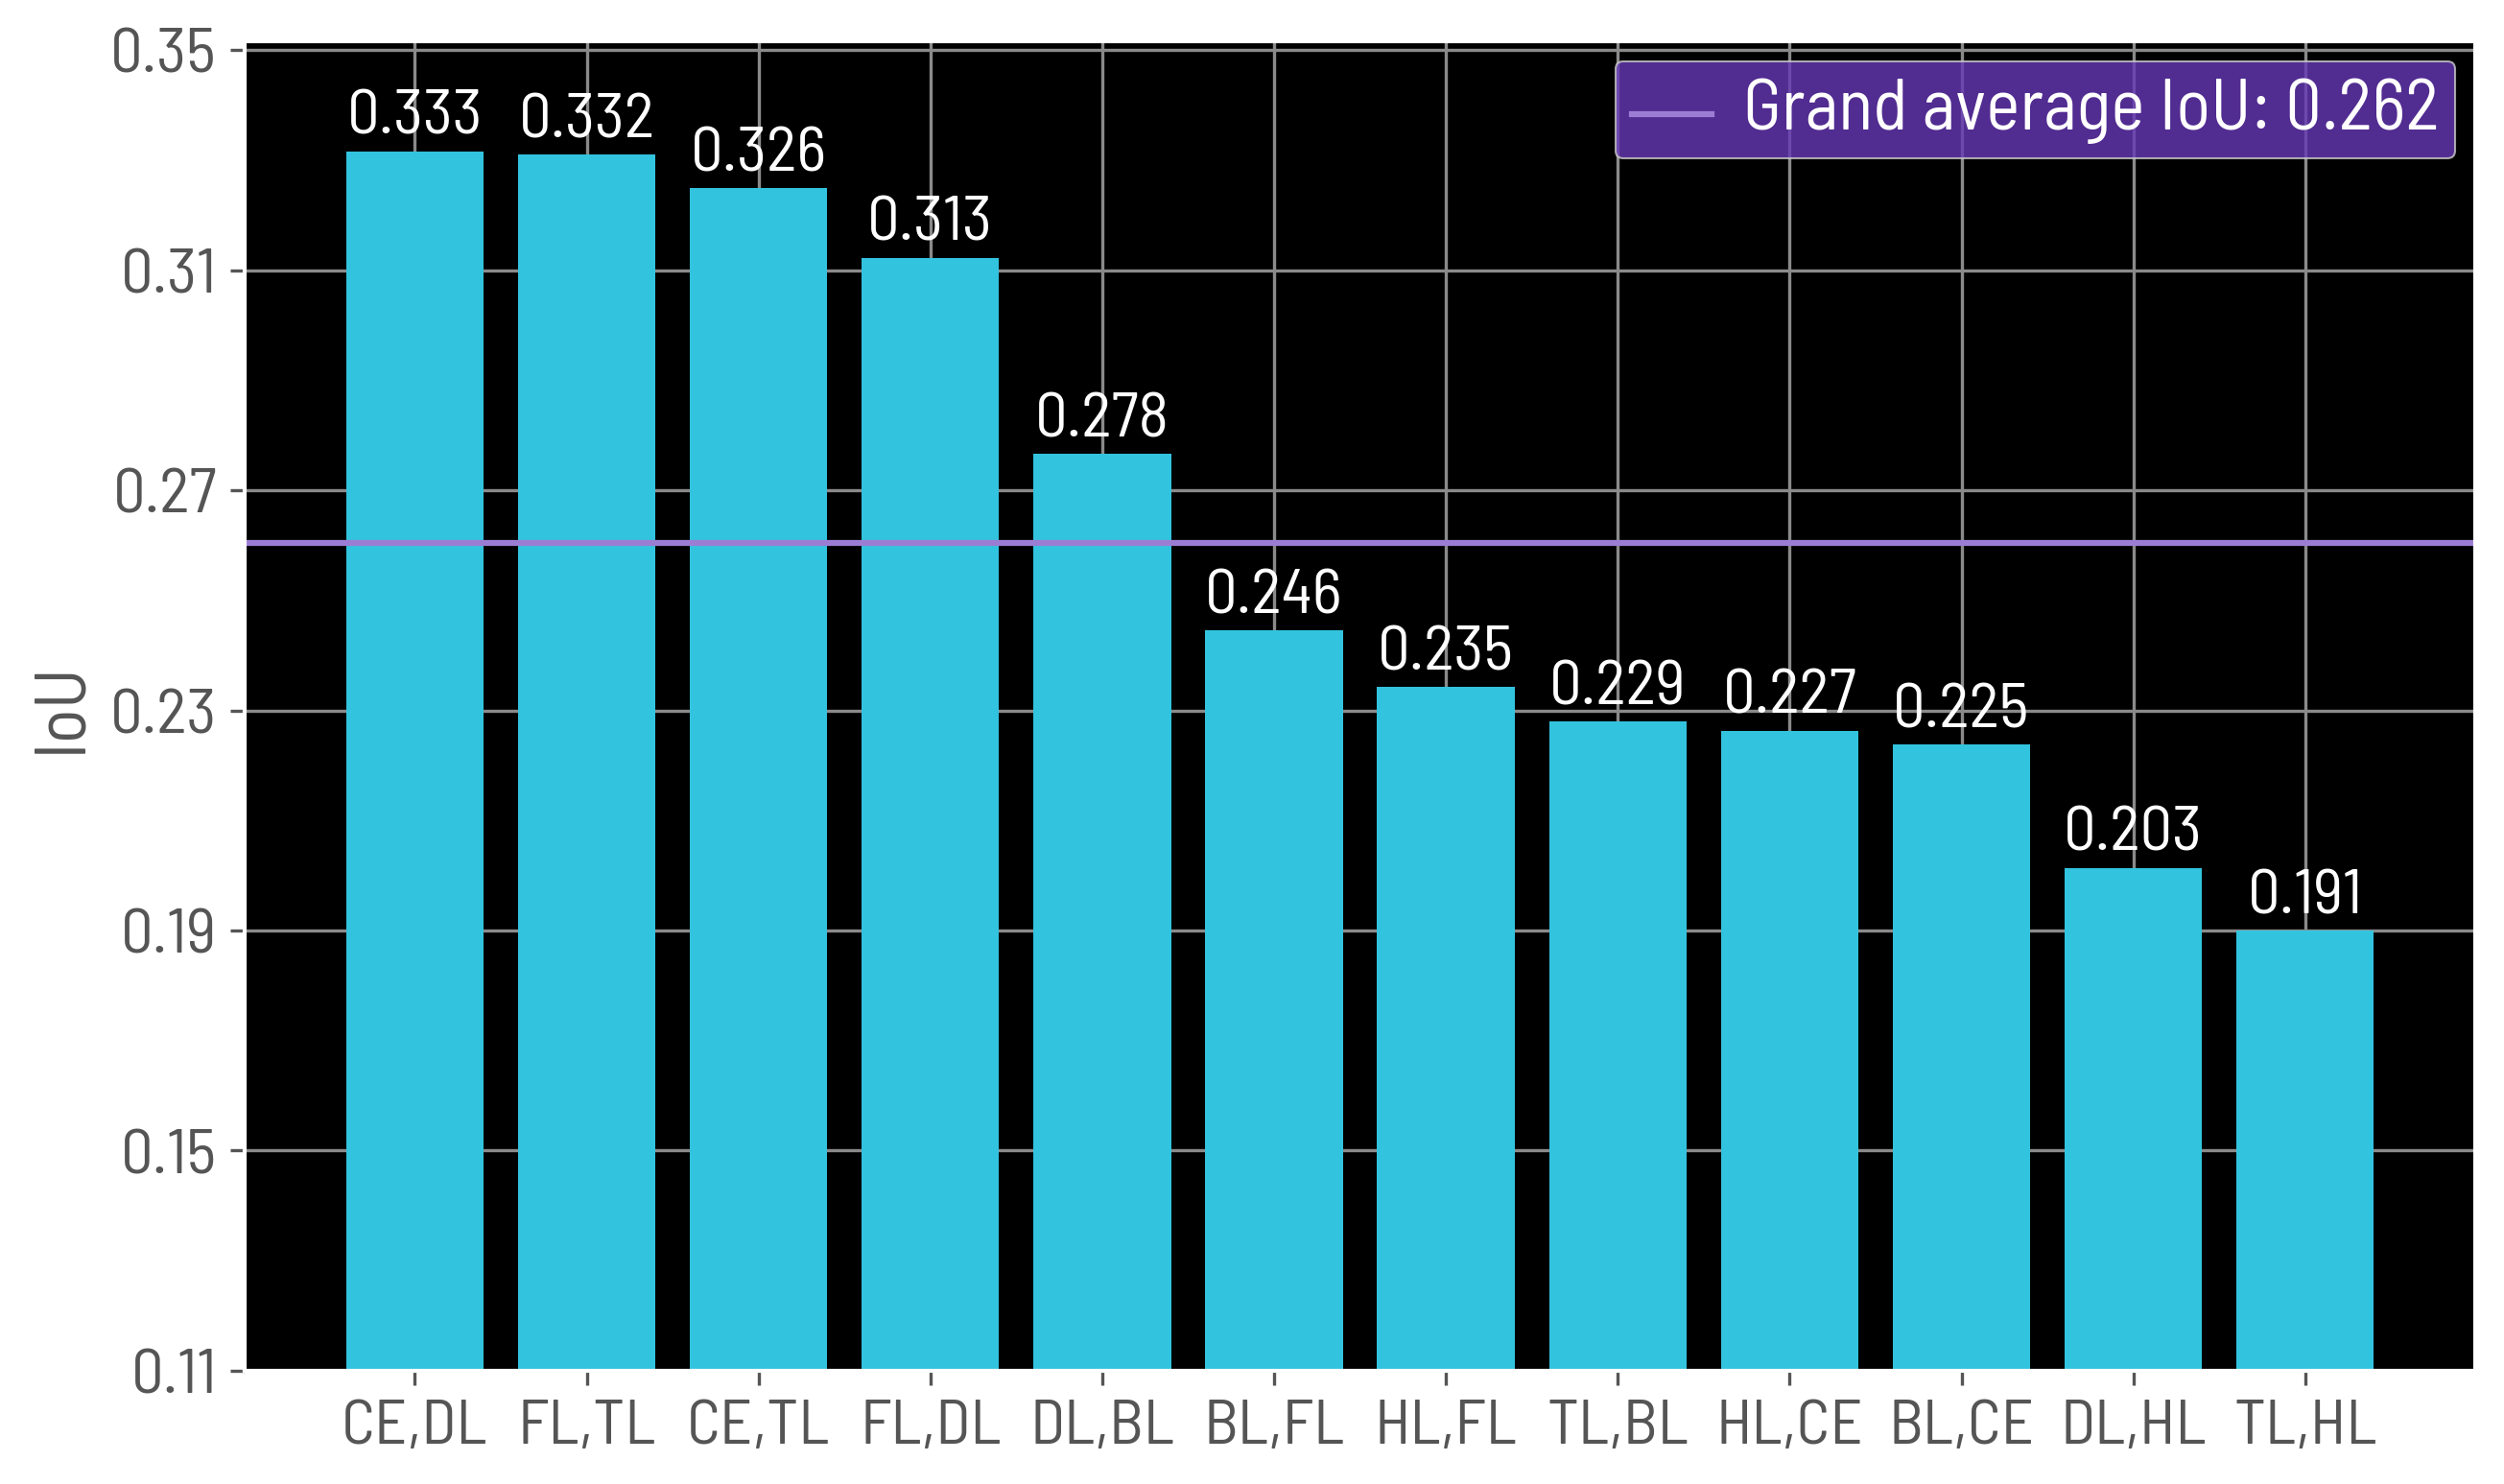
\includegraphics[width=\imgWidthcustom]{images/loss_combination_results_idrid_double_short_total.png}}
  \subfigure[Average IoU for Each Triple Loss Combination]{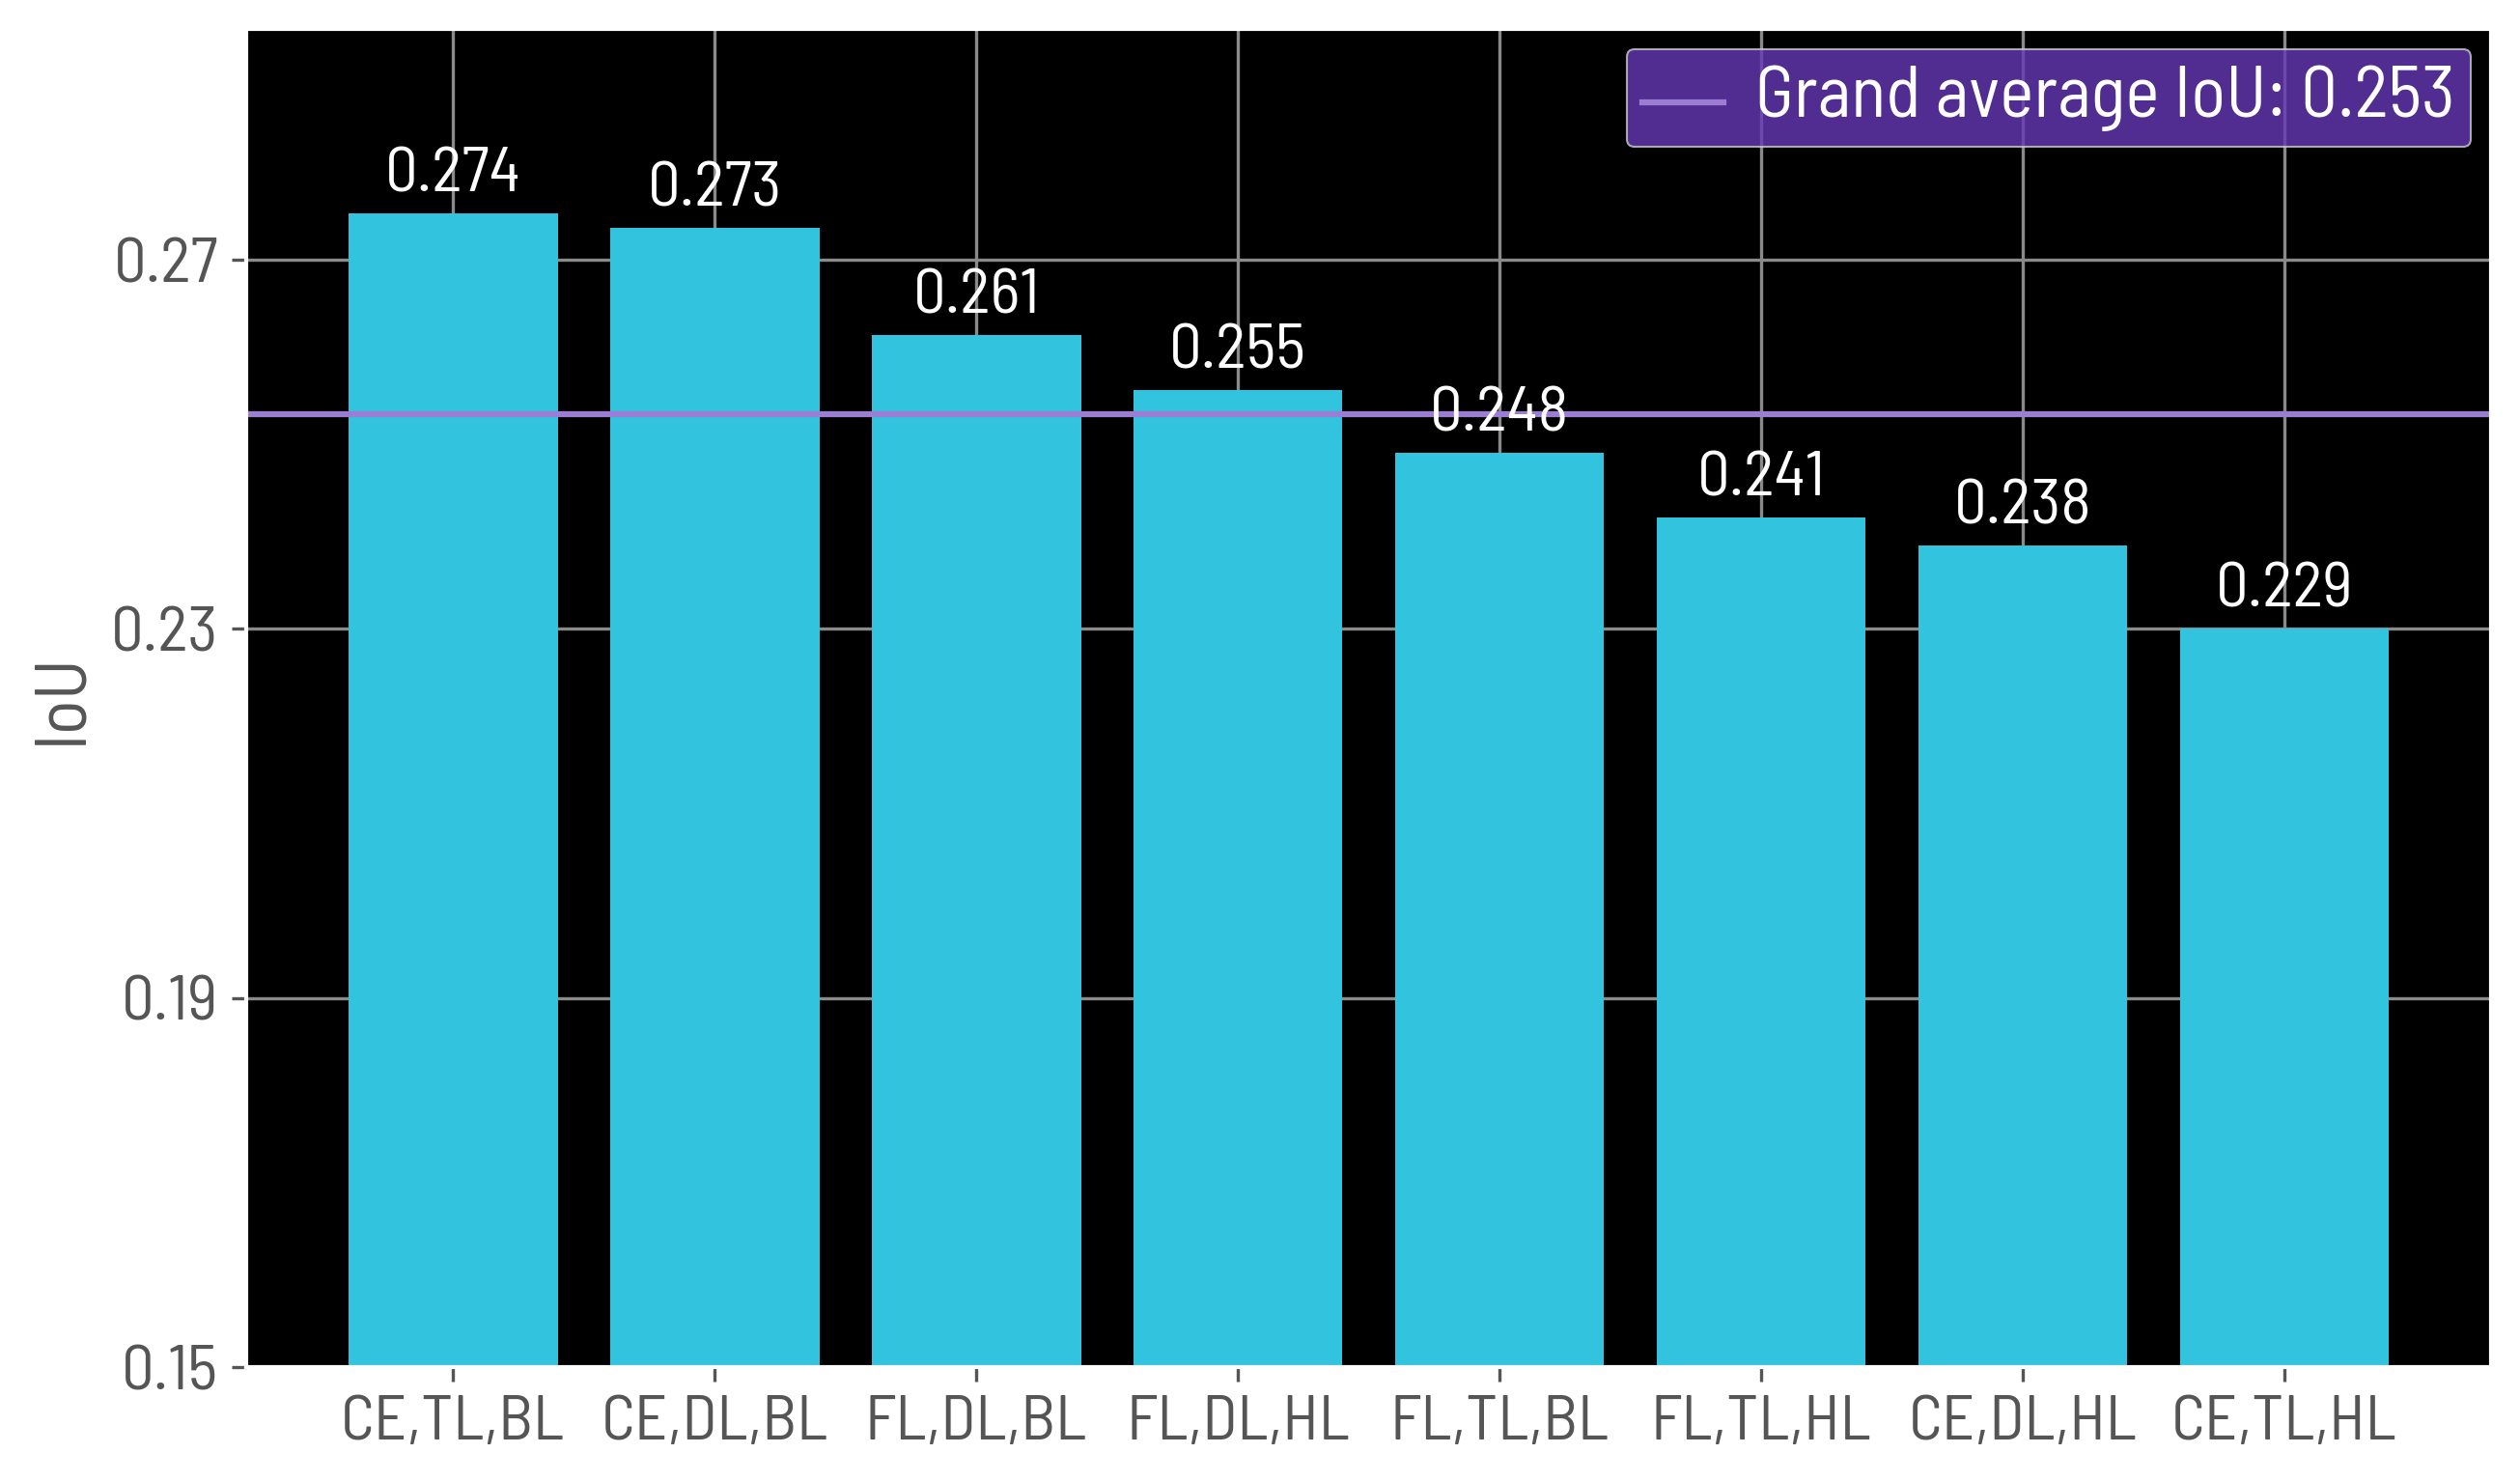
\includegraphics[width=\imgWidthcustom]{images/loss_combination_results_idrid_triple_short_total.png}}
  \caption[Average IoU for Loss Combination (IDRID)]{The figures showcase the average \ac{IoU} for loss combination, derived from an extensive set of 240 models trained on the \acf{IDRID}.}
  \label{discrete_loss_combination_results_idrid_short}
\end{figure}
\textbf{Merge strategy results}\newline
\figref{discrete_merge_strategy_results_idrid_short} showcases the average \ac{IoU} for each merge strategy. The averaging and static weighting strategies outperform others, while the extreme point strategies lag. Interestingly, despite the overall low performance of the MAX strategy, table \ref{tab:merge_strategy_results_idrid_double_long} reveals that it was used by the second-highest performing models (No. 7,8,9). A closer examination of \ref{overall_double_triple_idrid}, displaying the overall results heatmap, reveals a mixed performance for the MAX strategy, with some decent outcomes counterbalanced by several poor ones.
\begin{figure}[H]%[htbp]
  \centering
  \subfigure[Average IoU for Each Double Merge Strategy]{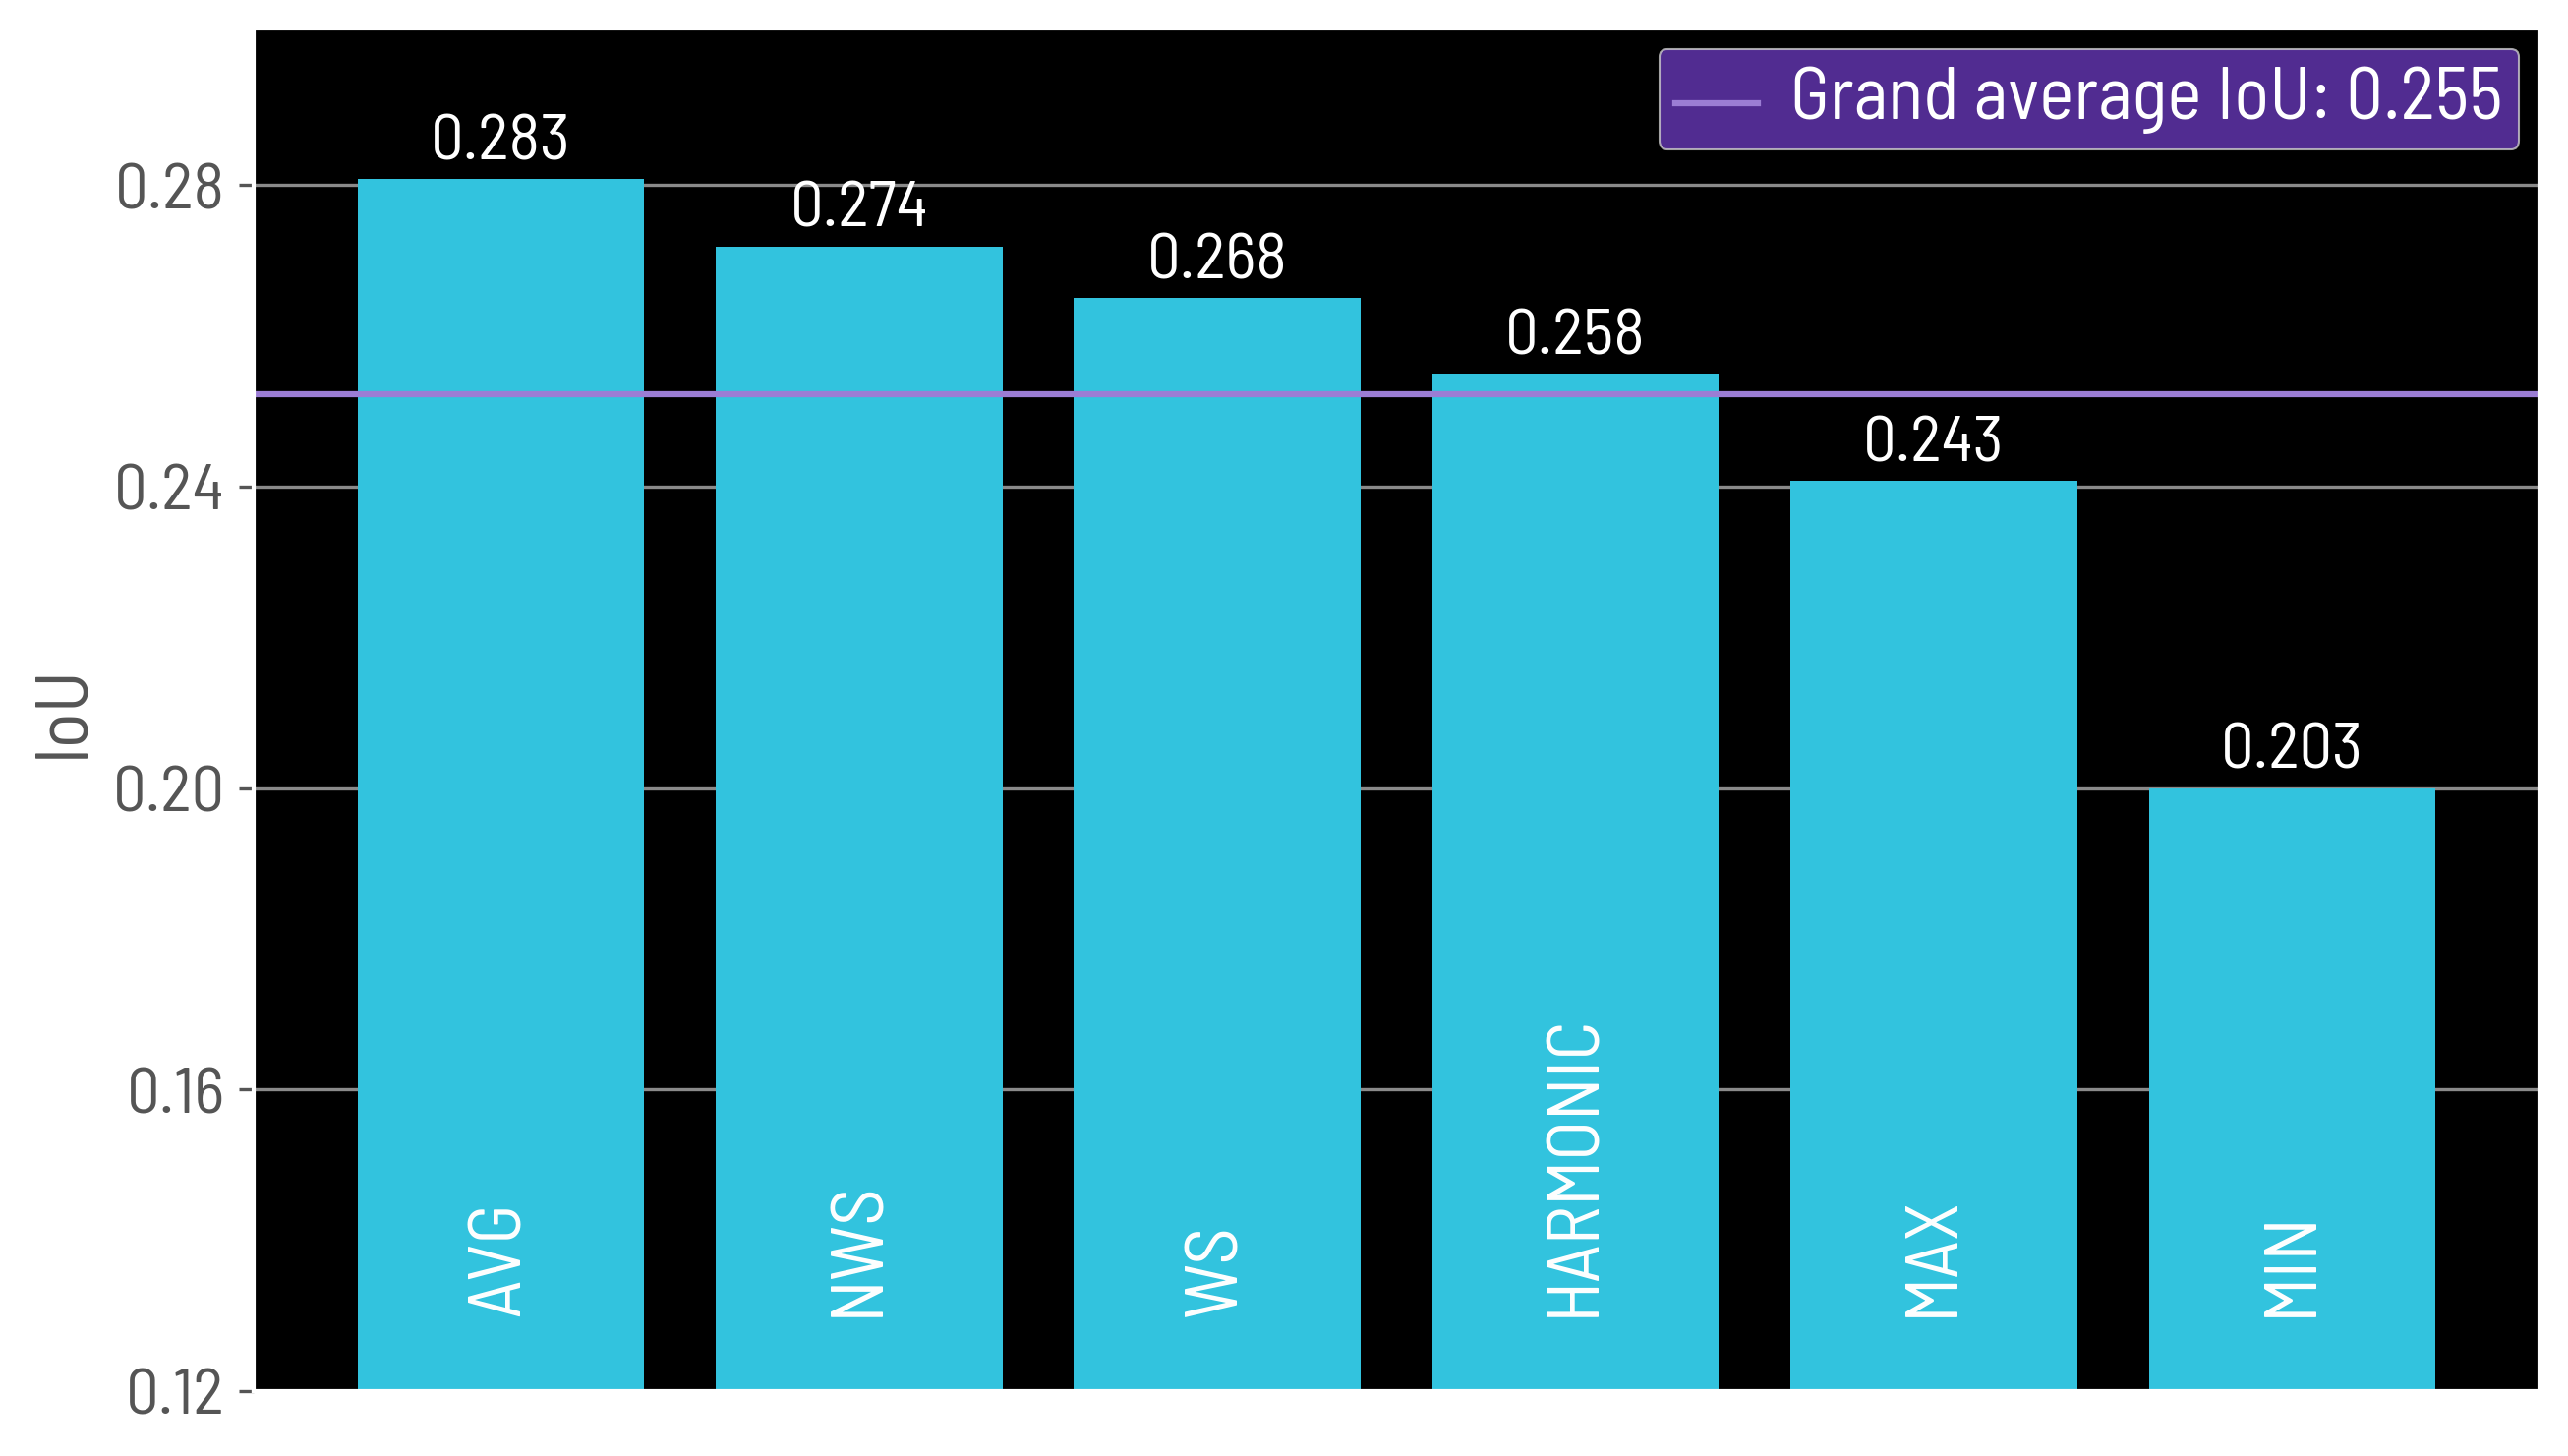
\includegraphics[width=\imgWidthcustom]{images/merge_strategy_results_idrid_double_short_total.png}}
  \subfigure[Average IoU for Each Triple Merge Strategy]{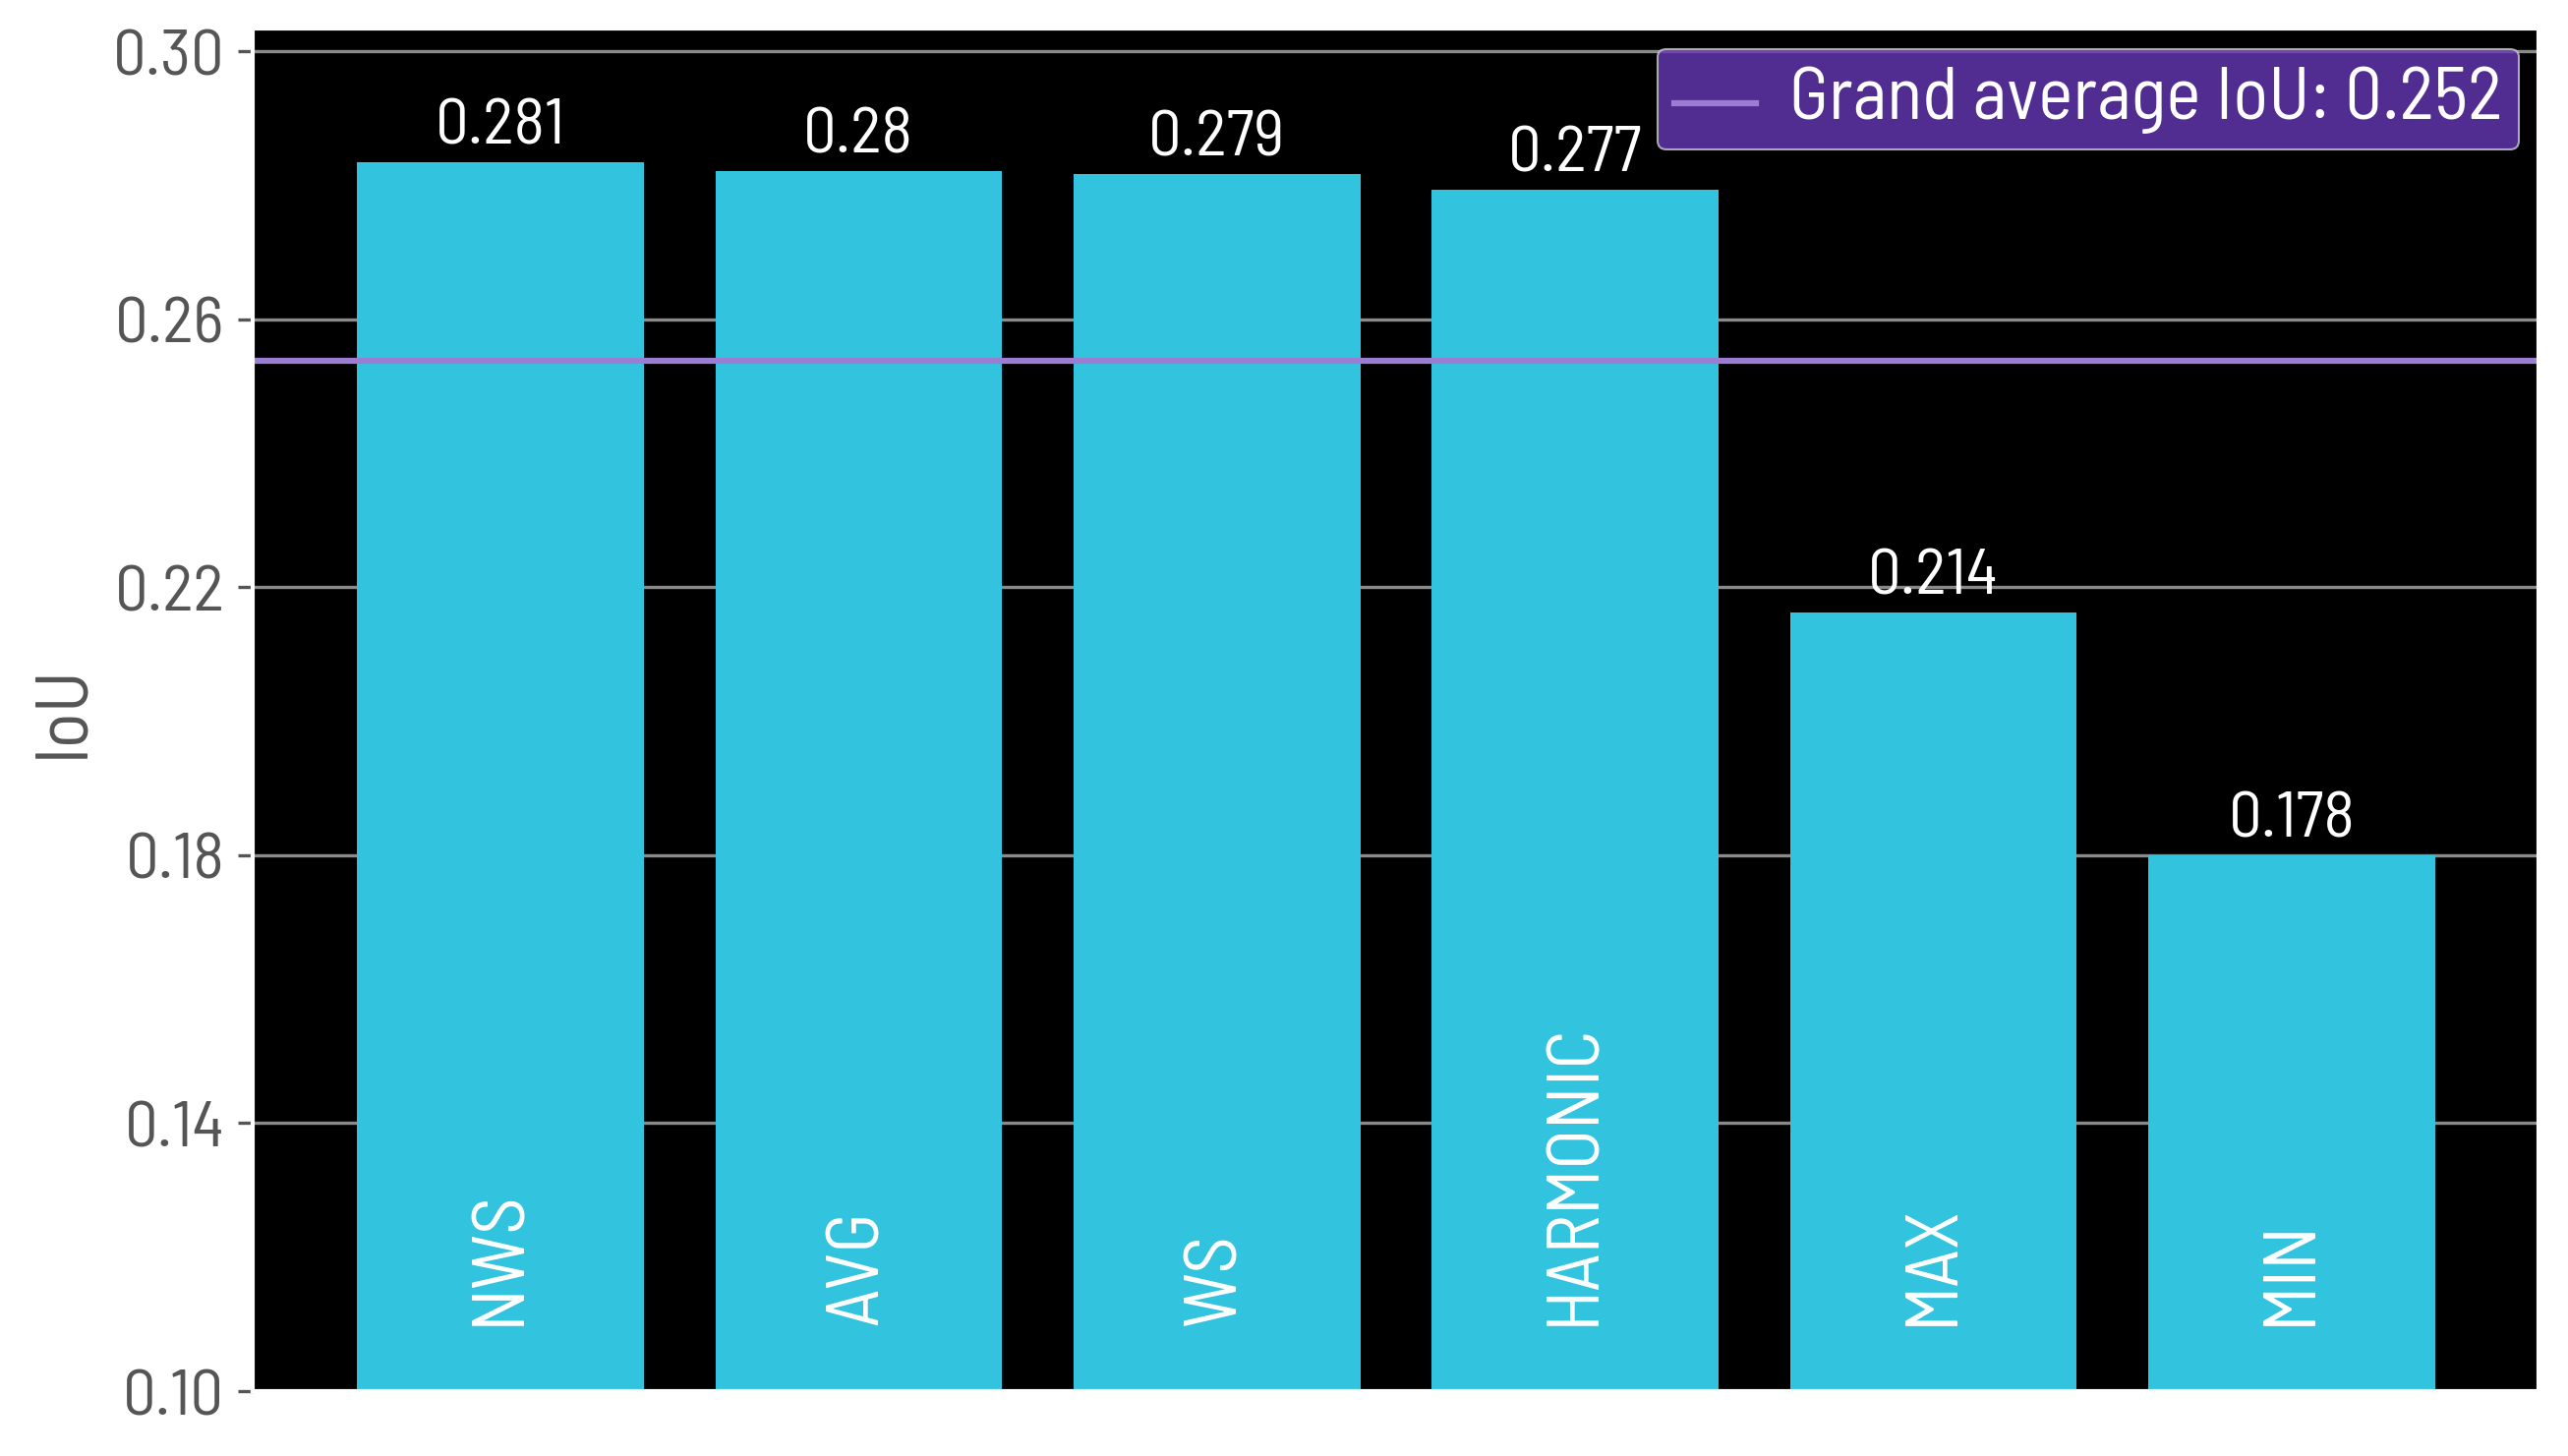
\includegraphics[width=\imgWidthcustom]{images/merge_strategy_results_idrid_triple_short_total.png}}
  \caption[Average IoU for Each Merge Strategy (IDRID)]{The figures showcase the average \ac{IoU} for each merge strategy, derived from an extensive set of 240 models trained on the \acf{IDRID}.}
  \label{discrete_merge_strategy_results_idrid_short}
\end{figure}

%----------------------------------CONTINOUS PERFORMANCE (Idrid)-------------------------%
\subsubsection*{Continuous Performance}
\figref{continous_results_total_idrid} presents the average performance for each loss function, employing the performance-based merge strategy from configuration no. 13 as outlined in \ref{tab:final_configuration_list}. The graph also highlights the model count for each loss combination, which is significantly larger for the \ac{IDRID} dataset, owing to its reduced computational resource requirements. The Hyperband search algorithm preferentially selected combinations that showed promise, as evidenced by the higher model count associated with combinations that achieved a greater average \ac{IoU}. However, the overall performance of the performance-based strategy was noticeably lower than that of the top-performing discrete strategies, partly due to a few underperforming combinations such as BL, CE, or TL, BL in the double loss combination results.

Despite the different model counts and the need to traverse a continuous hyperparameter space, making a direct comparison to discrete strategies challenging, some insights can still be gained. Although the average performance was somewhat low, table \ref{tab:continous_loss_combination_idrid_double_long} reveals that several high-performing models could match those from the discrete configurations, demonstrating the efficacy of the hyperparameter selection in the performance-based strategy.
\begin{figure}[H]%[htbp]
  \centering
  \subfigure[Average IoU for Each Double Loss Combination]{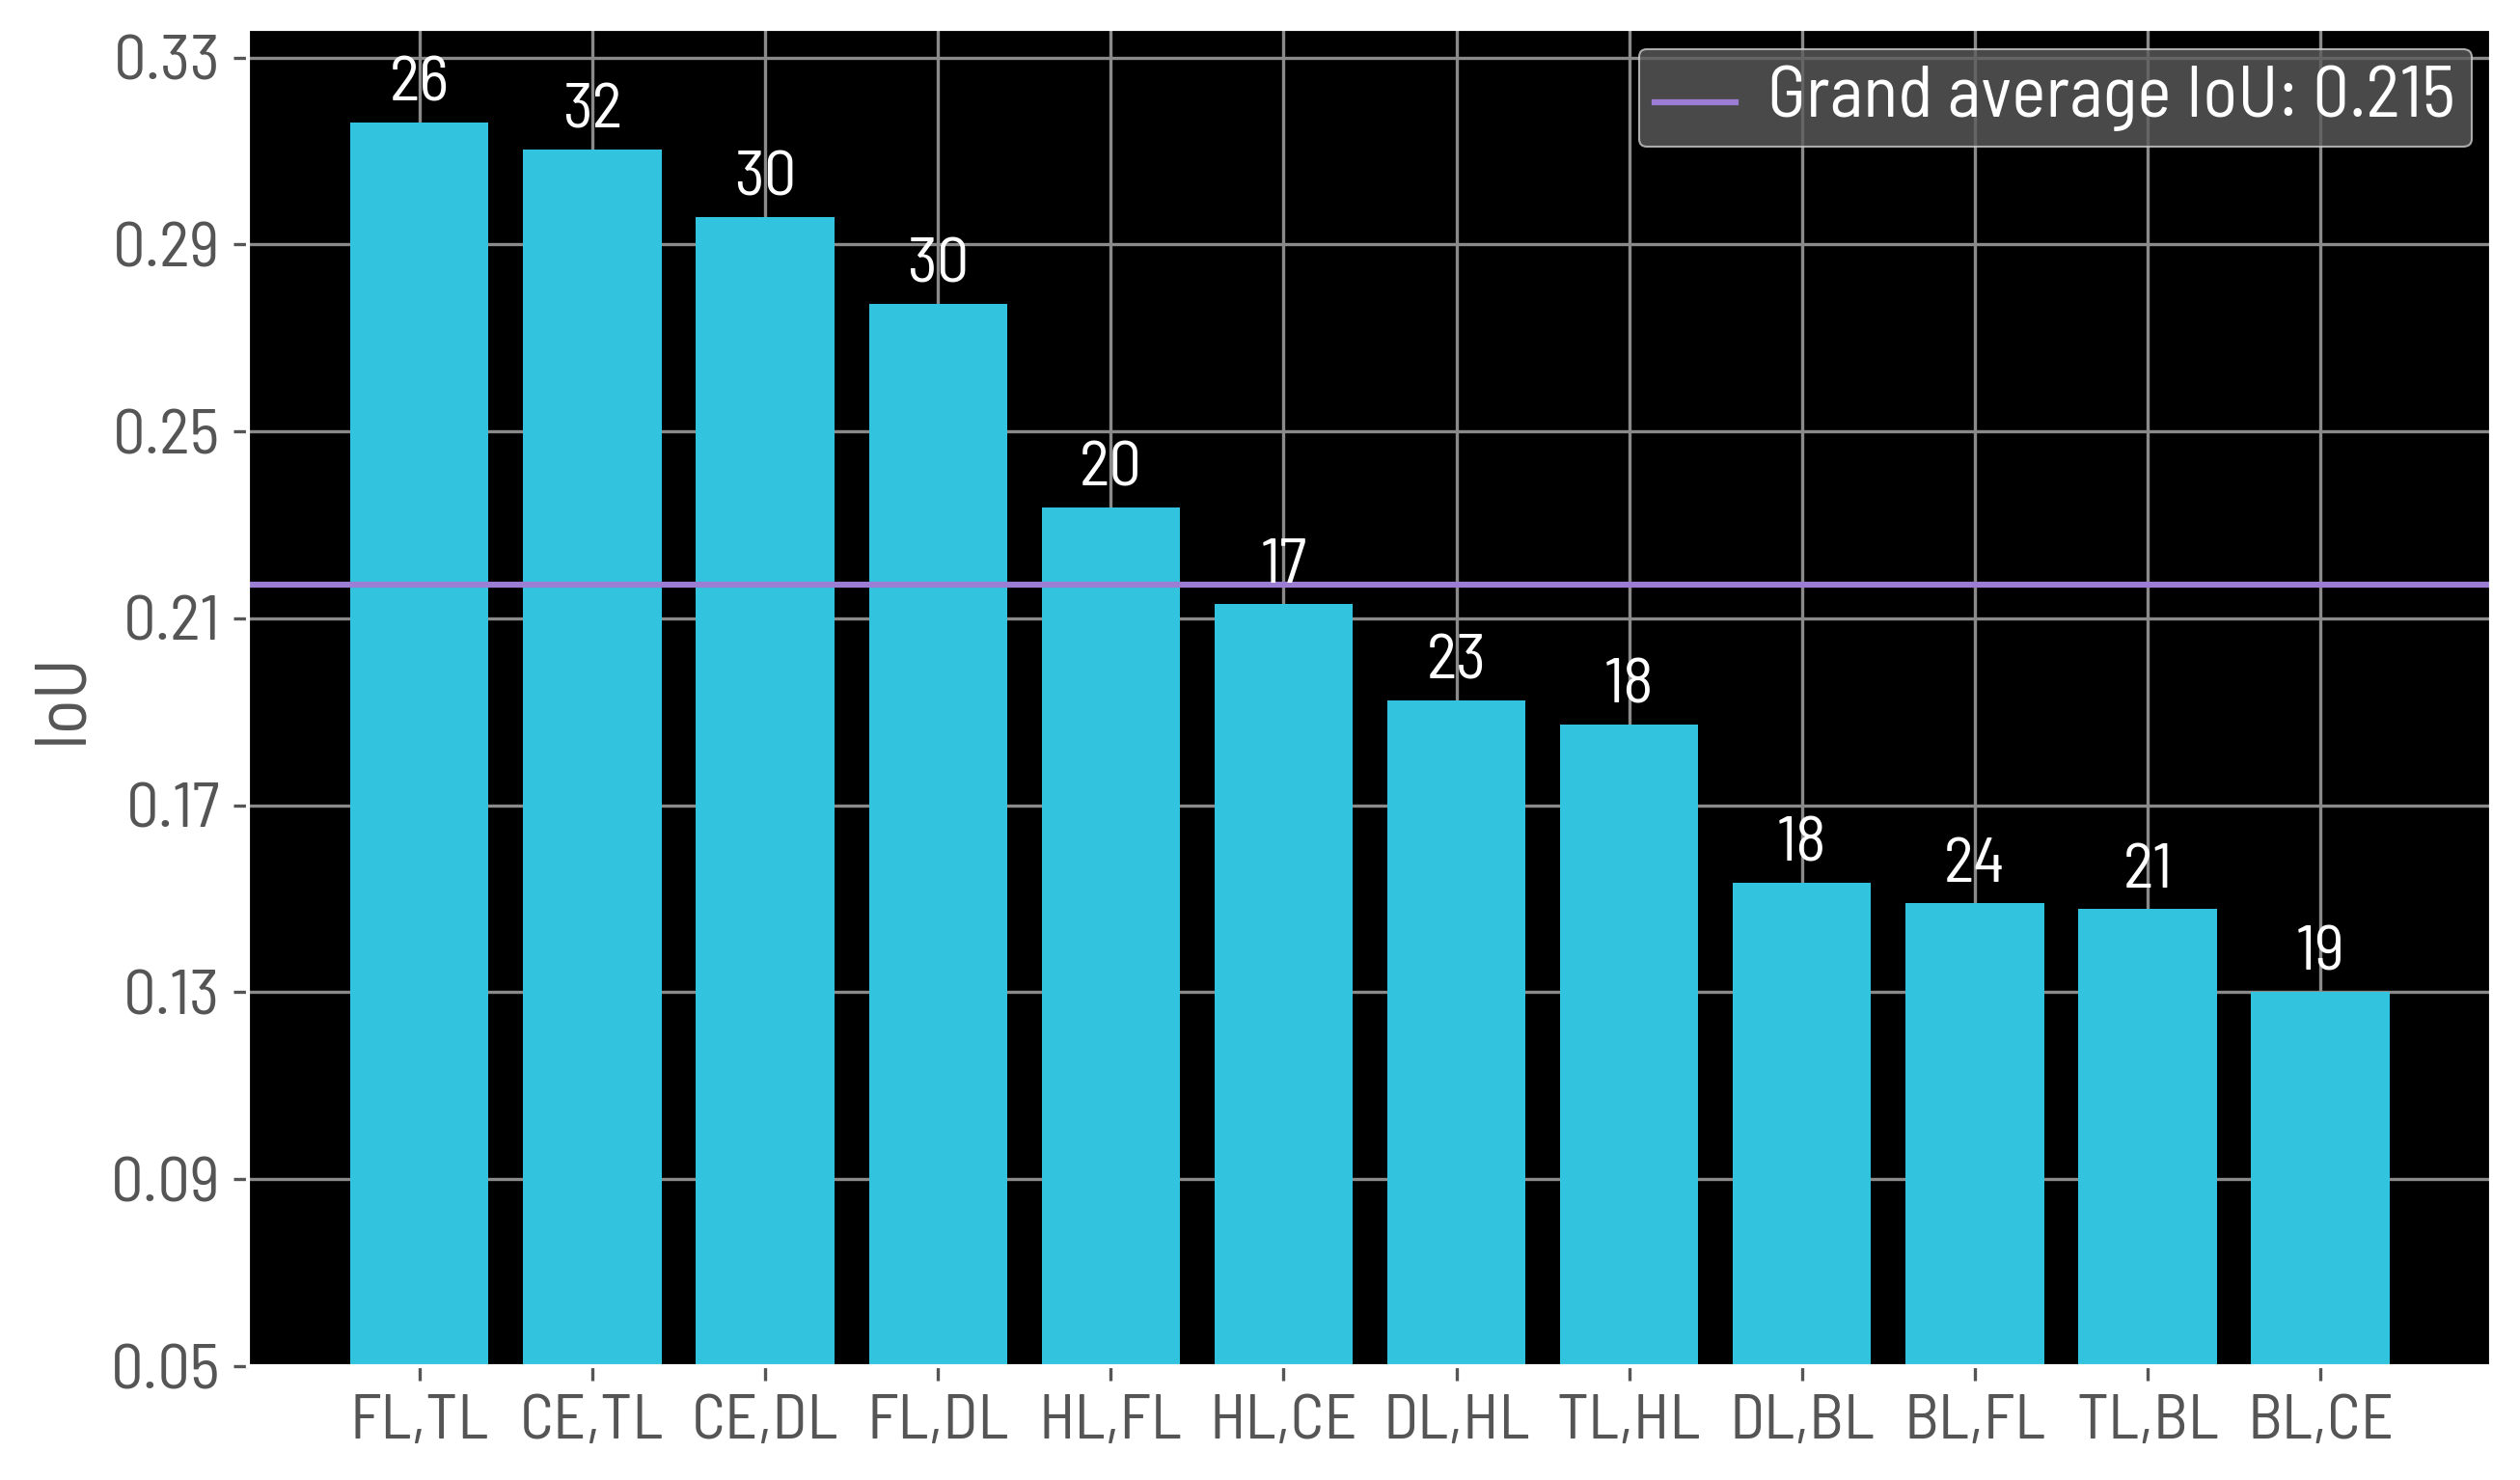
\includegraphics[width=\imgWidthcustom]{images/continous_loss_combination_results_idrid_double_short_total.png}}
  \subfigure[Average IoU for Each Triple Loss Combination]{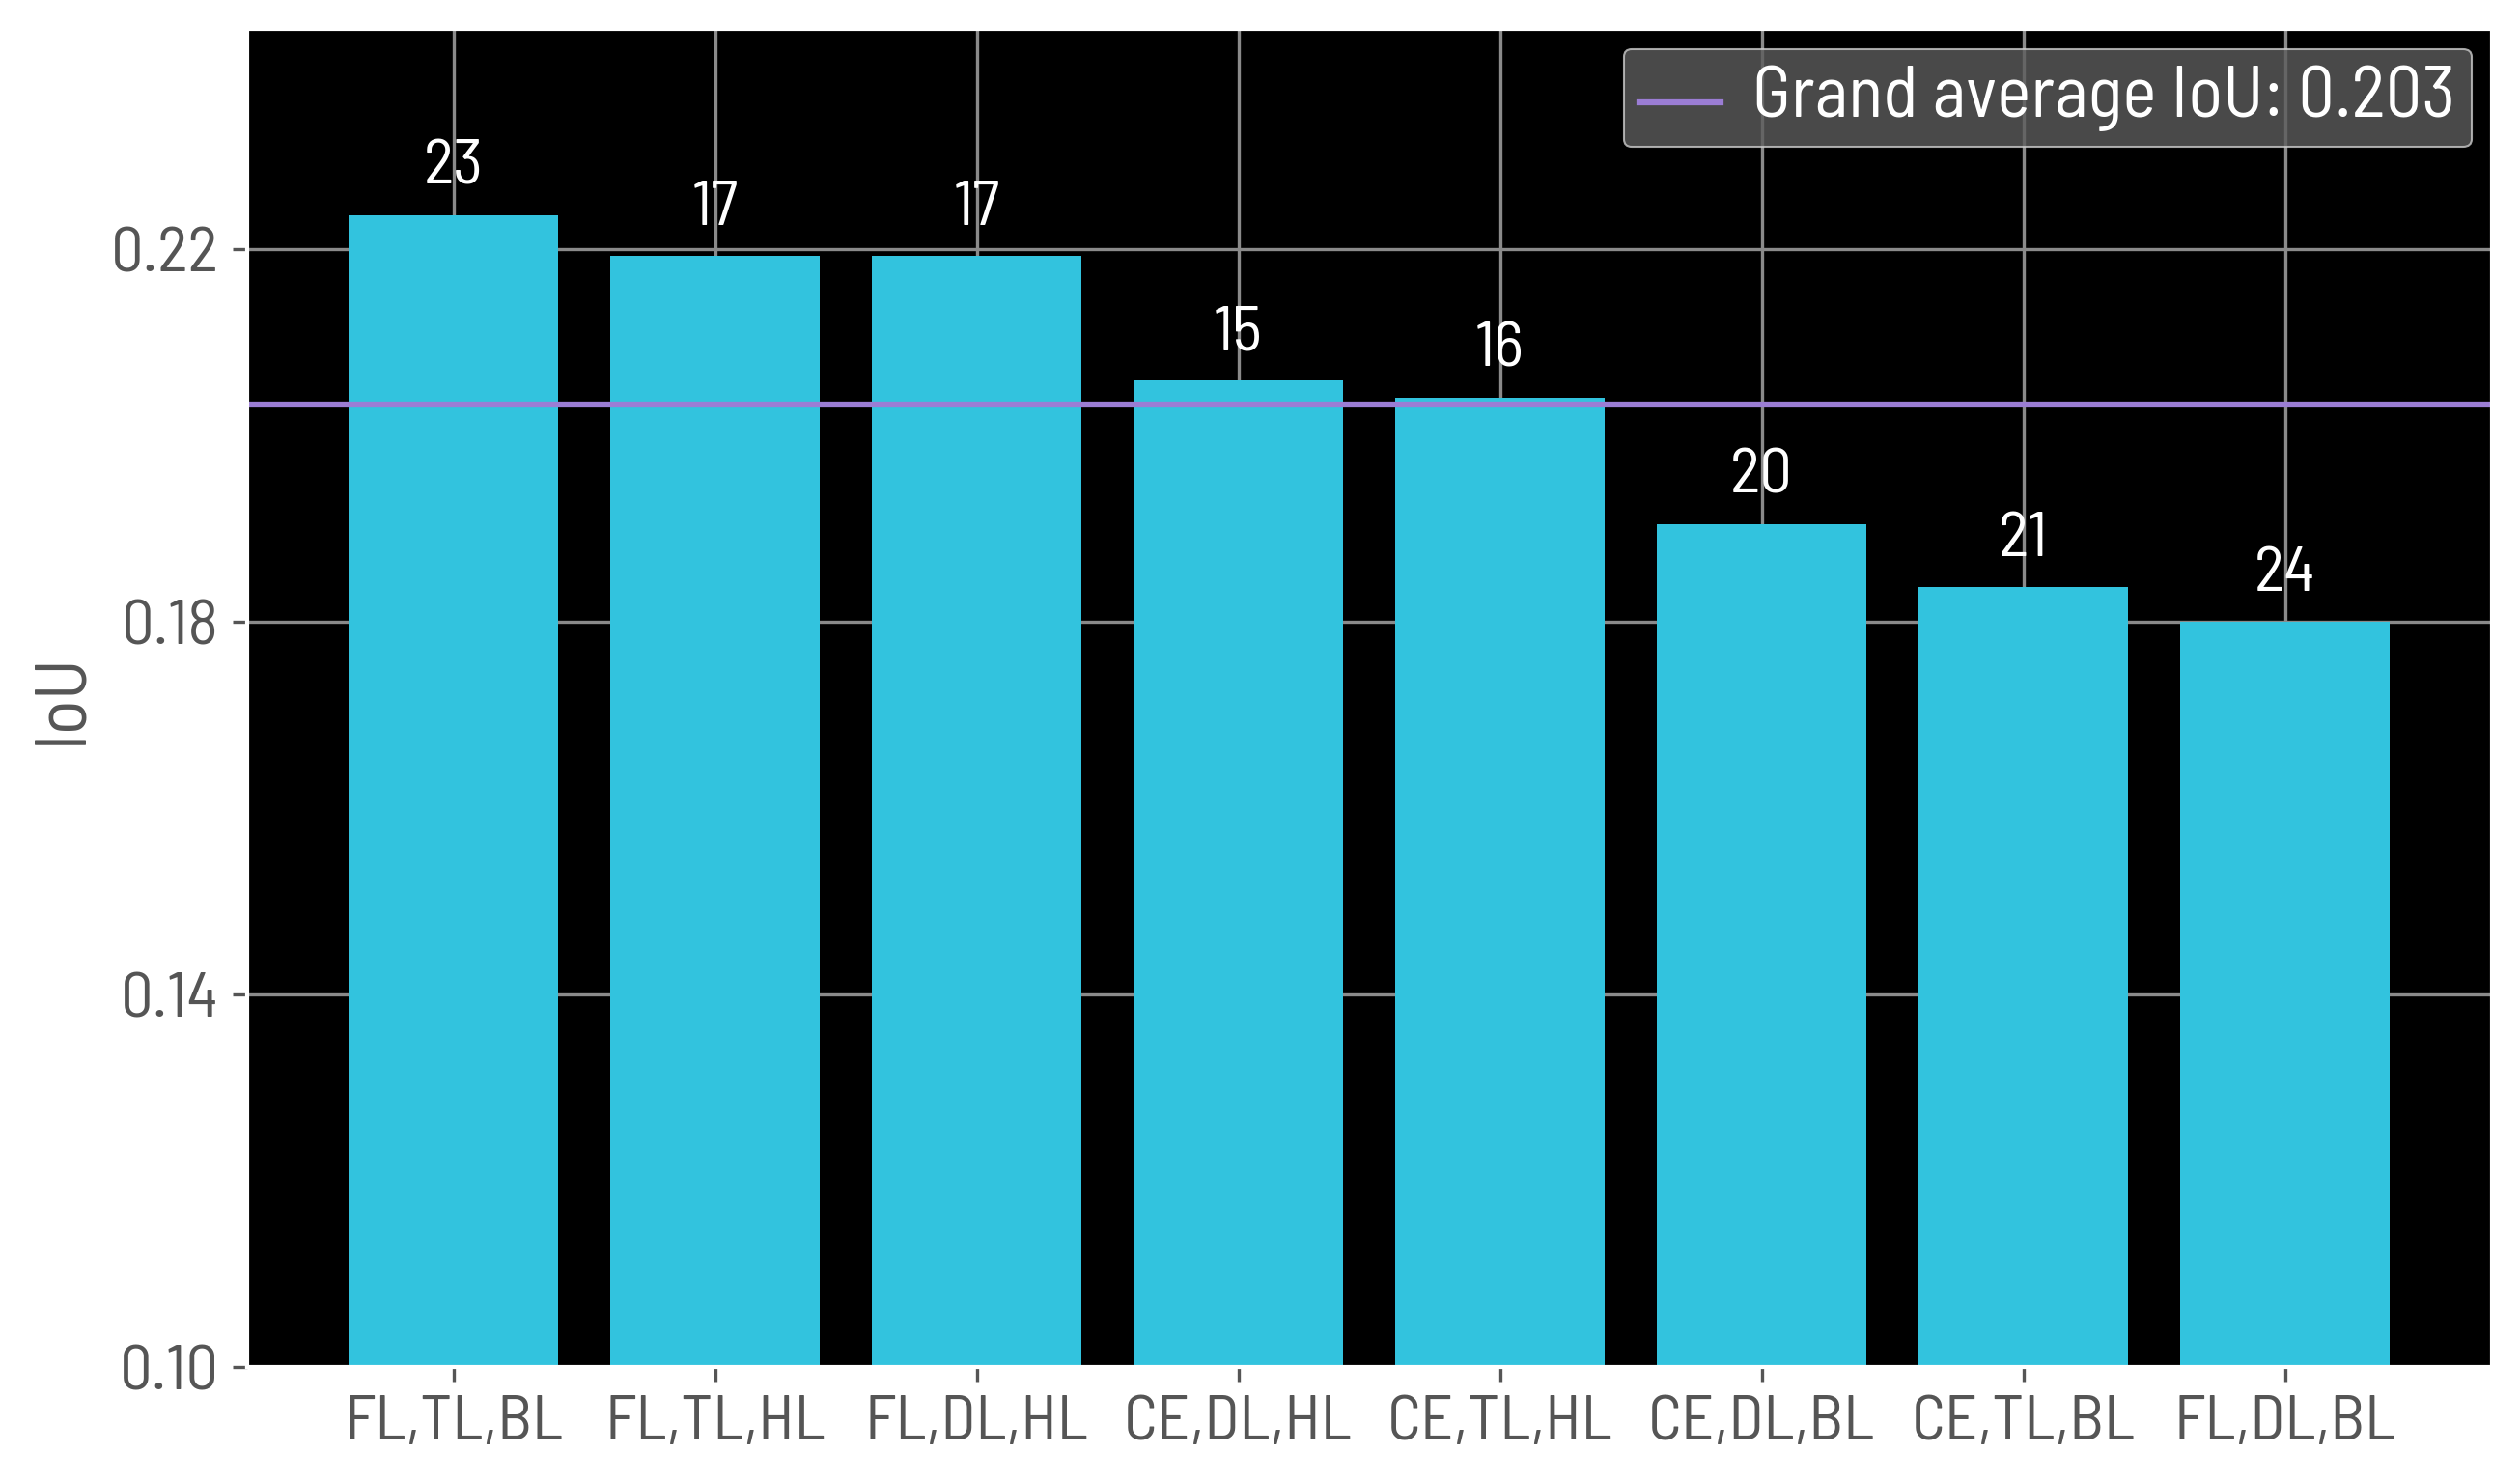
\includegraphics[width=\imgWidthcustom]{images/continous_loss_combination_results_idrid_triple_short_total.png}}
  \caption[Average IoU for Loss Combination (IDRID)]{The figures showcase the average \ac{IoU} for loss combination, derived from an extensive set of 432 models trained on the \acf{IDRID} using the performance-based merge strategy.}
  \label{continous_loss_combination_results_idrid_short}
\end{figure}
\figref{continous_results_total_idrid} shows the average \ac{IoU} corresponding to different model counts, illustrating a notable trend that a \texttt{pbm\_I} value approximating one yields better performance. The results concerning \texttt{pbm\_alpha} indicate optimal performance around $6.5$. Upon reviewing the top-performing results enumerated in table \ref{tab:continous_loss_combination_idrid_double_long} and table \ref{tab:continous_loss_combination_idrid_triple_long}, it is observed that the average values for \texttt{pbm\_alpha} and \texttt{pbm\_I} were $3.57$ and $0.795$ for the former, and $4.448$ and $0.802$ for the latter, respectively.

\begin{figure}[H]%[htbp]
  \centering
  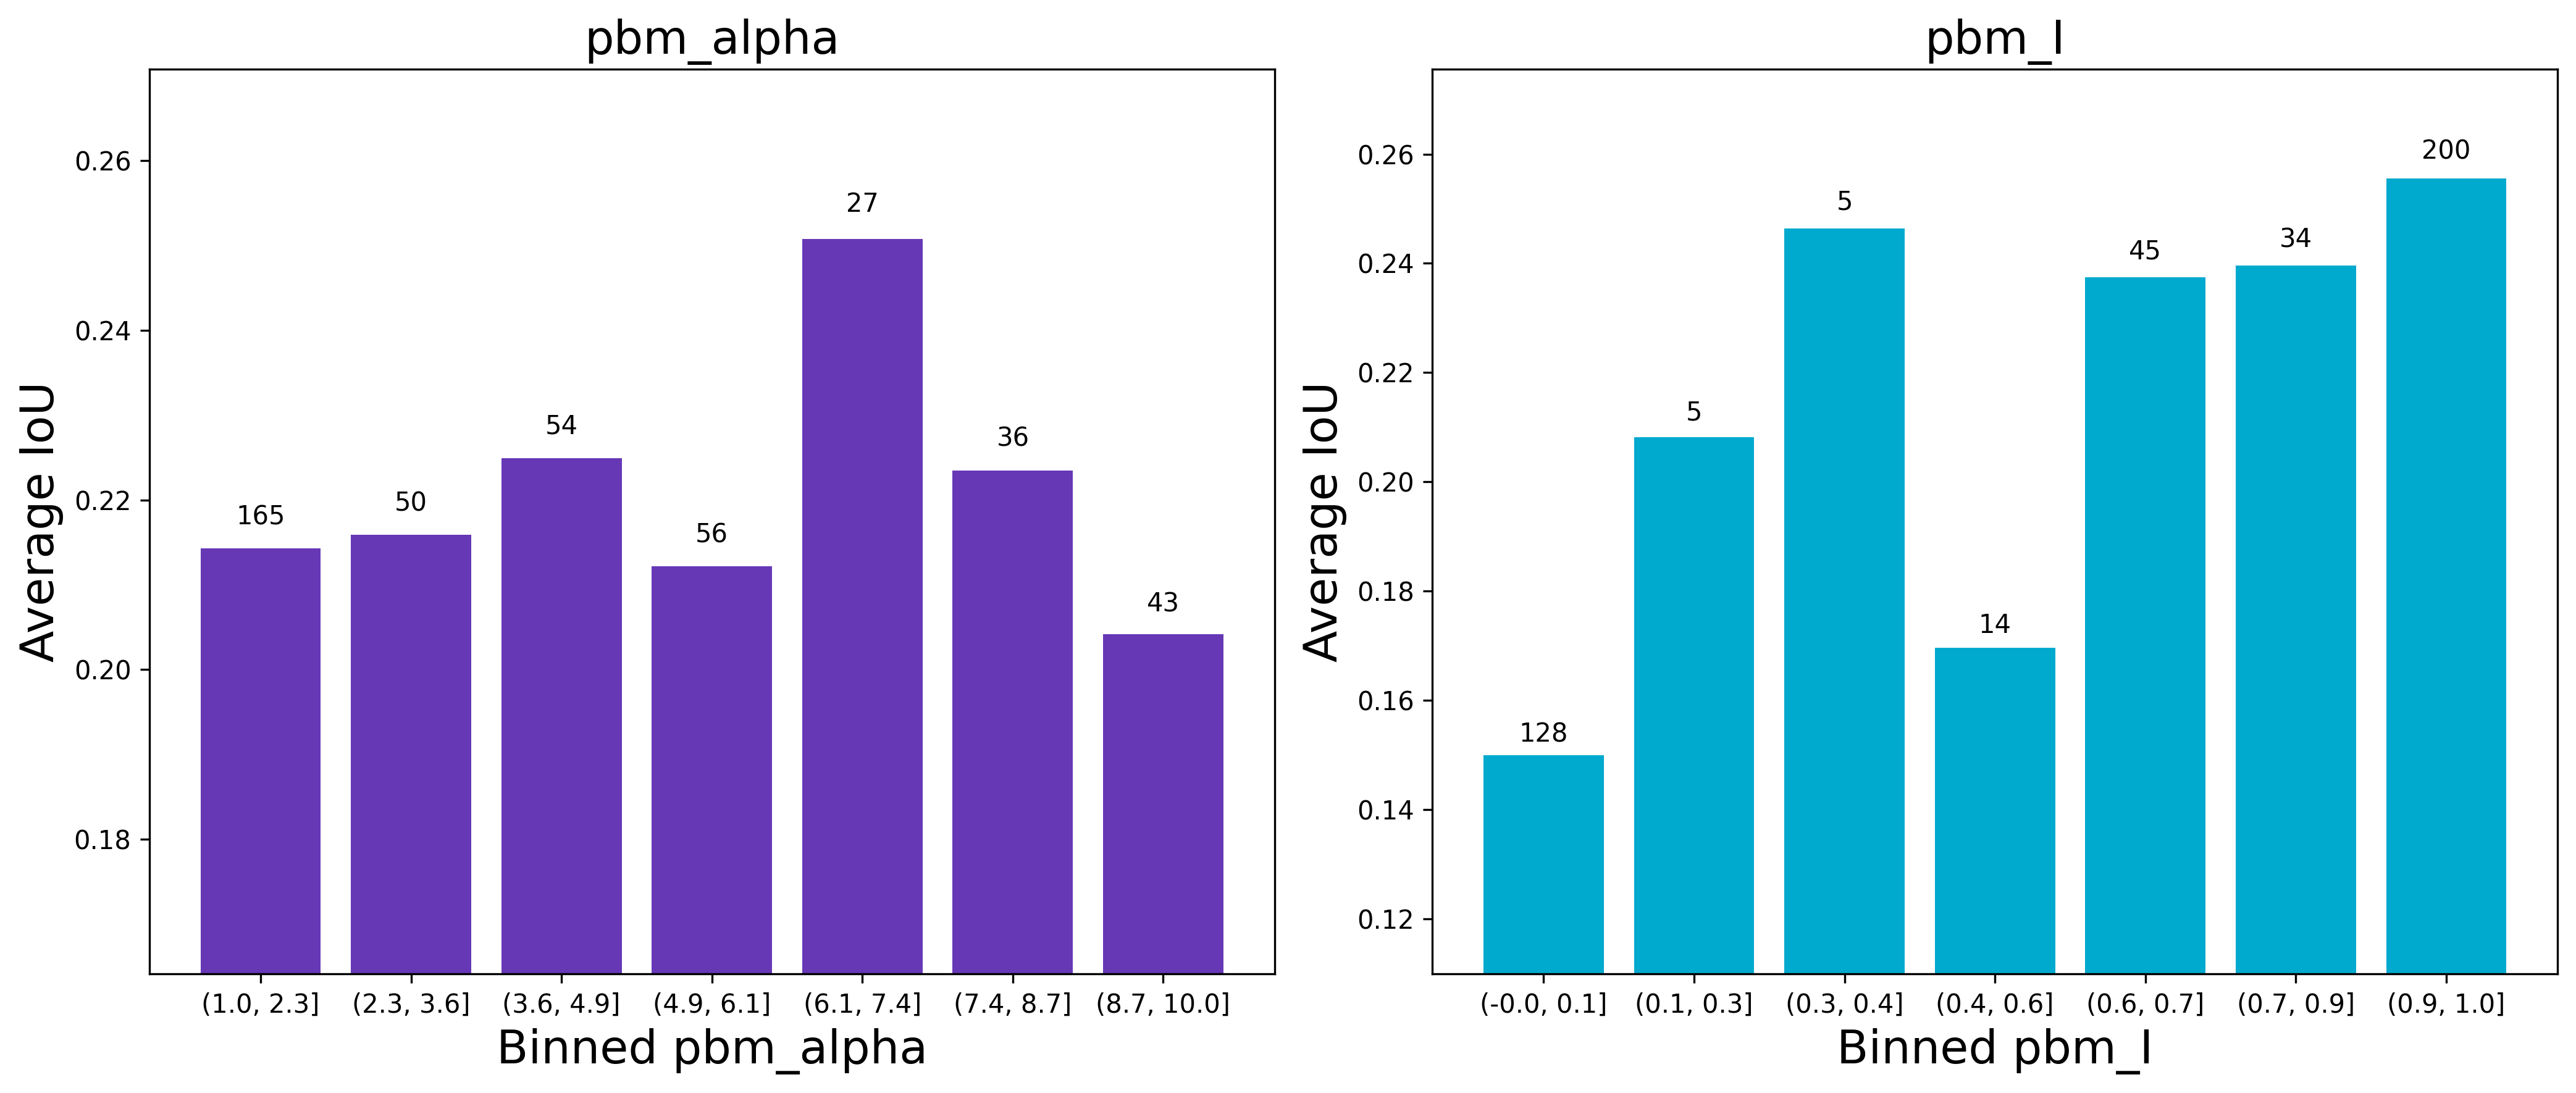
\includegraphics[width=\imgWidthL]{images/continous_hyperparameter_total_idrid.png}
  \caption[Hyperparameter analysis]{Hyperparameter analysis for performance-based merging. The x-axis corresponds to the hyperparameter \texttt{pbm\_alpha} and \texttt{pbm\_I} defined in table \ref{tab:hyperparameters} and \secref{sec:configuration}. Both values are float with \texttt{pbm\_alpha} $\in (1,10]$ and \texttt{pbm\_I}$\in [0,1]$. The bars are labeled with the model count and represent the average \ac{IoU} for the indicated range.}
  \label{continous_results_total_idrid}
\end{figure}

\subsubsection*{Specific Performance}
As a specific loss-merge combination for the specific configuration no.15 defined in table \ref{tab:final_configuration_list}, the AVG strategy along the combinations of \ac{CE} and \ac{DL} was used, and resulted in a grand average of $0.38$ for 6 models trained, failing to reach the discrete by 1\% but outperforming the best baseline average by 3.9\%. The detailed results for each model can be viewed in \secref{subsec:specific_combination_idrid}.
%----------------------------------------------------------------------------------------%
%---------------------------------------Qualitative results------------------------------%
%----------------------------------------------------------------------------------------%
\section{Qualitative Results}
\label{sec:qualitative_results}
This section offers a comprehensive overview and qualitative analysis of the results derived from the proposed framework across the suggested datasets. The visual examination of these outcomes can be critical, as it enables a quick and intuitive understanding of the model's performance, identifies its shortcomings, and potentially signals system bugs. A qualitative review can also reveal issues that numerical metrics overlook, enabling the user to enrich the understanding of the model's capabilities.

While the principal aim was to show if the proposed implementation outperforms the standard baseline methods, detecting a visual performance increase may be challenging, mainly if improvements are minimal. Nevertheless, the subsequent sections will analyze five inputs for each dataset predicted by a baseline model and a model using the proposed loss merging framework.
%--------------------------------------MEDAKA--------------------------------------------%
\subsection{Medaka Fish}
% Please add the following required packages to your document preamble:
% \usepackage{graphicx}
% \usepackage[table,xcdraw]{xcolor}
% If you use beamer only pass "xcolor=table" option, i.e. \documentclass[xcolor=table]{beamer}
\begin{table}[H]
    \centering
    \resizebox{\textwidth}{!} &
      {\color[HTML]{FFFFFF} Strategy} &
      {\color[HTML]{FFFFFF} IoU} &
      {\color[HTML]{FFFFFF} IoU 0} &
      {\color[HTML]{FFFFFF} IoU 1} &
      {\color[HTML]{FFFFFF} IoU 2} &
      {\color[HTML]{FFFFFF} IoU 3} &
      {\color[HTML]{FFFFFF} PPV} &
      {\color[HTML]{FFFFFF} TPR} &
      {\color[HTML]{FFFFFF} PPV vs. TPR} \\ \hline
    1 &
      73 &
      CE &
      1.00 &
      - &
      0.697 &
      0.974 &
      0.756 &
      0.471 &
      0.586 &
      0.807 &
      0.832 &
      TPR \\ \hline
    2 &
      138 &
      HD,FL &
      1.00 &
      AVG &
      0.762 &
      0.984 &
      0.751 &
      0.607 &
      0.705 &
      0.874 &
      0.834 &
      PPV \\ \hline
    \end{tabular}%
    }
    \caption[Quantitative results for qualitative analysis (Medaka)]{The table presents two distinct models that will be used in this section for a qualitative comparison. Model no.1 is constructed using a baseline setup, while model no.2 has been trained with the proposed loss merging framework. The columns $IoU_0,\hdots,IoU_3$ represent the four classes, Background, Bulbus, Atrium and Ventricle.  The column titled \squote{PPV vs. TPR} illustrates the trade-off between a high \acf{PPV} and low \acf{TPR}, or vice versa, for each model.}
    \label{tab:qualitative_comparison_medaka}
    \end{table}
\figref{ce_medaka_base} displays the qualitative results of a baseline model trained on the \acf{MFD}. From Table \ref{tab:qualitative_comparison_medaka}, we observe that model no. 1 achieved an \ac{IoU} score of $0.697$, which is approximately 2\% higher than the top-performing baseline averages discussed in \secref{subsec:medaka_fish}. The Bulbus class exhibited the best prediction, with an \ac{IoU} score of 0.756. The images reveal minimal false positives for this class, indicating the model's superior recall performance compared to its precision.
\begin{figure}[H]%[htbp]
  \centering  
  \subfigure[]{
\includegraphics[width=\imgWidthFive]{images/ce_medaka_base/mask/ce_medaka_base_2_blended.png}}
  \subfigure[]{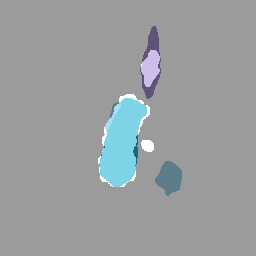
\includegraphics[width=\imgWidthFive]{images/ce_medaka_base/mask/ce_medaka_base_3_blended.png}}
  \subfigure[]{
\includegraphics[width=\imgWidthFive]{images/ce_medaka_base/mask/ce_medaka_base_5_blended.png}}
  \subfigure[]{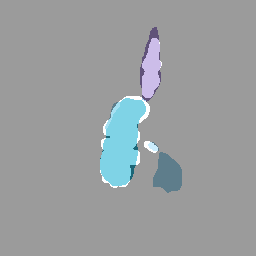
\includegraphics[width=\imgWidthFive]{images/ce_medaka_base/mask/ce_medaka_base_11_blended.png}}
  \subfigure[]{
\includegraphics[width=\imgWidthFive]{images/ce_medaka_base/mask/ce_medaka_base_18_blended.png}}
  \subfigure[]{\includegraphics[width=\imgWidthFive]{images/ce_medaka_base/input/rgb_mask_viewing_2_8de5348dd06ac1441888.png}}
  \subfigure[]{\includegraphics[width=\imgWidthFive]{images/ce_medaka_base/input/rgb_mask_viewing_3_3743a94d8a3da2ecb289.png}}
  \subfigure[]{\includegraphics[width=\imgWidthFive]{images/ce_medaka_base/input/rgb_mask_viewing_5_056a64513a2f6835d029.png}}
  \subfigure[]{\includegraphics[width=\imgWidthFive]{images/ce_medaka_base/input/rgb_mask_viewing_11_b5989a70492fd8b8d20a.png}}
  \subfigure[]{\includegraphics[width=\imgWidthFive]{images/ce_medaka_base/input/rgb_mask_viewing_18_c64c26a866df90443831.png}}
  \caption[Quantitative baseline analysis for the \ac{MFD}]{Image (a) to (e) illustrate baseline predictions as colored masks against the inverse of the ground truth mask colored in grey. We can see three classes to predict named \textbf{\textcolor{rwuvioletlight}{Bulbus}}, \textbf{\textcolor{rwucyan40}{Atrium}} and \textbf{\textcolor{rwucyan}{Ventricle}}. The corresponding quantitative results are listed in table \ref{tab:qualitative_comparison_medaka} as model no.1. Image (f) to (j) depict the input features for each prediction above.}
  \label{ce_medaka_base}
\end{figure}
\figref{hlfl_medaka_lossCombo} showcases the qualitative results of a model that has been trained using a combination of \ac{HL} and \ac{FL}, employing the arithmetic averaging strategy. The model attains an \ac{IoU} score of $0.762$. Compared to the baseline model, it achieves considerably higher precision, particularly noticeable for the Atrium class in images (a) through (e). Additionally, the Ventricle class improved significantly by 11.9\%.

\begin{figure}[H]%[htbp]
  \centering  
  \subfigure[]{
\includegraphics[width=\imgWidthFive]{images/hlfl_medaka_lossCombo/mask/hlfl_medaka_lossCombo_2_blended.png}}
  \subfigure[]{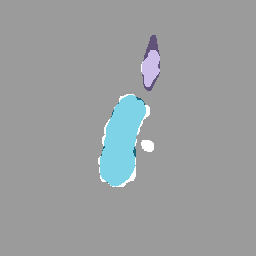
\includegraphics[width=\imgWidthFive]{images/hlfl_medaka_lossCombo/mask/hlfl_medaka_lossCombo_3_blended.png}}
  \subfigure[]{
\includegraphics[width=\imgWidthFive]{images/hlfl_medaka_lossCombo/mask/hlfl_medaka_lossCombo_5_blended.png}}
  \subfigure[]{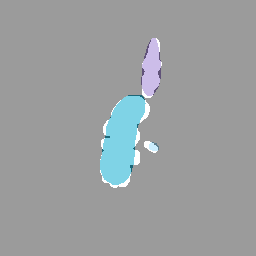
\includegraphics[width=\imgWidthFive]{images/hlfl_medaka_lossCombo/mask/hlfl_medaka_lossCombo_11_blended.png}}
  \subfigure[]{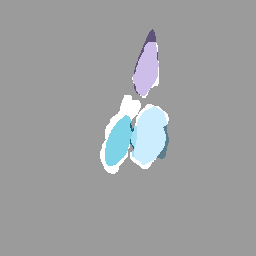
\includegraphics[width=\imgWidthFive]{images/hlfl_medaka_lossCombo/mask/hlfl_medaka_lossCombo_18_blended.png}}
  \subfigure[]{\includegraphics[width=\imgWidthFive]{images/hlfl_medaka_lossCombo/input/rgb_mask_viewing_2_8de5348dd06ac1441888.png}}
  \subfigure[]{\includegraphics[width=\imgWidthFive]{images/hlfl_medaka_lossCombo/input/rgb_mask_viewing_3_3743a94d8a3da2ecb289.png}}
  \subfigure[]{\includegraphics[width=\imgWidthFive]{images/hlfl_medaka_lossCombo/input/rgb_mask_viewing_5_056a64513a2f6835d029.png}}
  \subfigure[]{\includegraphics[width=\imgWidthFive]{images/hlfl_medaka_lossCombo/input/rgb_mask_viewing_11_b5989a70492fd8b8d20a.png}}
  \subfigure[]{\includegraphics[width=\imgWidthFive]{images/hlfl_medaka_lossCombo/input/rgb_mask_viewing_18_c64c26a866df90443831.png}}
  \caption[Quantitative loss merging analysis for the \ac{MFD}]{Image (a) to (e) illustrate loss merging predictions as colored masks against the inverse of the ground truth mask colored in grey. We can see three classes to predict named \textbf{\textcolor{rwuvioletlight}{Bulbus}}, \textbf{\textcolor{rwucyan40}{Atrium}} and \textbf{\textcolor{rwucyan}{Ventricle}}. The corresponding quantitative results are listed in table \ref{tab:qualitative_comparison_medaka} as model no.2. Image (f) to (j) depict the input features for each prediction above.}
  \label{hlfl_medaka_lossCombo}
\end{figure}
%--------------------------------------SKIN LESION---------------------------------------%
\subsection{Skin Lesion}
% Please add the following required packages to your document preamble:
% \usepackage{graphicx}
% \usepackage[table,xcdraw]{xcolor}
% If you use beamer only pass "xcolor=table" option, i.e. \documentclass[xcolor=table]{beamer}
\begin{table}[H]
  \centering
  \resizebox{\textwidth}{!} &
    {\color[HTML]{FFFFFF} Strategy} &
    {\color[HTML]{FFFFFF} IoU} &
    {\color[HTML]{FFFFFF} IoU 0} &
    {\color[HTML]{FFFFFF} IoU 1} &
    {\color[HTML]{FFFFFF} PPV} &
    {\color[HTML]{FFFFFF} TPR} &
    {\color[HTML]{FFFFFF} PPV vs. TPR} \\ \hline
  1 &
    158 &
    Focal &
    0.64 &
     &
    0.659 &
    0.821 &
    0.497 &
    0.832 &
    0.793 &
    PPV \\ \hline
  2 &
    185 &
    CE,TL &
    0.64 &
    NWS &
    0.671 &
    0.812 &
    0.529 &
    0.822 &
    0.814 &
    PPV \\ \hline
  \end{tabular}%
  }
  \caption[Quantitative results for qualitative analysis (Skin Lesion)]{The table presents two distinct models that will be used in this section for a qualitative comparison. Model no.1 is constructed using a baseline setup, while model no.2 has been trained with the proposed loss merging framework. The $IoU$ column reflects the average outcomes contrasting the foreground class against the background class where the columns $IoU_0,IoU_1$ represent the Background and Foreground class individually. The column titled \squote{PPV vs. TPR} illustrates the trade-off between a high \acf{PPV} and low \acf{TPR}, or vice versa, for each model.}
  \label{tab:qualitative_comparison_melanoma}
  \end{table}
\figref{ce_melanoma_baseV2} portrays the qualitative results of a baseline model (no. 1) that was trained using the \ac{FL}. The model obtained an \ac{IoU} score of $0.659$, which is 6.5\% higher than the average of the top-performing baselines discussed in \secref{subsec:skin_lesion}. The model also displayed a higher precision than recall, as evidenced by the PPV and TPR columns in Table \ref{tab:qualitative_comparison_medaka}. This attribute is reflected in the images, particularly in images (a) and (b), where a larger number of false negatives contribute to a lower true positive rate (TPR).
\begin{figure}[H]%[htbp]
  \centering  
  \subfigure[]{\includegraphics[width=\imgWidthFive]{images/ce_melanoma_baseV2/mask/ce_melanoma_baseV2_1_blended.png}}
  \subfigure[]{\includegraphics[width=\imgWidthFive]{images/ce_melanoma_baseV2/mask/ce_melanoma_baseV2_2_blended.png}}
  \subfigure[]{\includegraphics[width=\imgWidthFive]{images/ce_melanoma_baseV2/mask/ce_melanoma_baseV2_4_blended.png}}
  \subfigure[]{\includegraphics[width=\imgWidthFive]{images/ce_melanoma_baseV2/mask/ce_melanoma_baseV2_5_blended.png}}
  \subfigure[]{\includegraphics[width=\imgWidthFive]{images/ce_melanoma_baseV2/mask/ce_melanoma_baseV2_19_blended.png}}
  \subfigure[]{\includegraphics[width=\imgWidthFive]{images/ce_melanoma_baseV2/input/rgb_mask_viewing_1_ccf498805d88b46035f1.png}}
  \subfigure[]{\includegraphics[width=\imgWidthFive]{images/ce_melanoma_baseV2/input/rgb_mask_viewing_2_eea14c750494fcc06a17.png}}
  \subfigure[]{\includegraphics[width=\imgWidthFive]{images/ce_melanoma_baseV2/input/rgb_mask_viewing_4_8da635f3492a9f983465.png}}
  \subfigure[]{\includegraphics[width=\imgWidthFive]{images/ce_melanoma_baseV2/input/rgb_mask_viewing_5_4eafac7de3d2e7b2a1ba.png}}
  \subfigure[]{\includegraphics[width=\imgWidthFive]{images/ce_melanoma_baseV2/input/rgb_mask_viewing_19_78c8a248fd0b31e99ae9.png}}
  \caption[Quantitative baseline analysis for the \ac{SLD}]{Image (a) to (e) illustrate baseline predictions as colored masks against the inverse of the ground truth mask colored in grey. We can see one class to predict. The corresponding quantitative results are listed in table \ref{tab:qualitative_comparison_melanoma} as model no.1. Image (f) to (j) depict the input features for each prediction above.}
  \label{ce_melanoma_baseV2}
\end{figure}
\begin{figure}[H]%[htbp]
  \centering  
  \subfigure[]{\includegraphics[width=\imgWidthFive]{images/cetl_melanoma_lossCombo/mask/cetl_melanoma_lossCombo_1_blended.png}}
  \subfigure[]{\includegraphics[width=\imgWidthFive]{images/cetl_melanoma_lossCombo/mask/cetl_melanoma_lossCombo_2_blended.png}}
  \subfigure[]{\includegraphics[width=\imgWidthFive]{images/cetl_melanoma_lossCombo/mask/cetl_melanoma_lossCombo_4_blended.png}}
  \subfigure[]{\includegraphics[width=\imgWidthFive]{images/cetl_melanoma_lossCombo/mask/cetl_melanoma_lossCombo_5_blended.png}}
  \subfigure[]{\includegraphics[width=\imgWidthFive]{images/cetl_melanoma_lossCombo/mask/cetl_melanoma_lossCombo_19_blended.png}}
  \subfigure[]{\includegraphics[width=\imgWidthFive]{images/cetl_melanoma_lossCombo/input/rgb_mask_viewing_1_ccf498805d88b46035f1.png}}
  \subfigure[]{\includegraphics[width=\imgWidthFive]{images/cetl_melanoma_lossCombo/input/rgb_mask_viewing_2_eea14c750494fcc06a17.png}}
  \subfigure[]{\includegraphics[width=\imgWidthFive]{images/cetl_melanoma_lossCombo/input/rgb_mask_viewing_4_8da635f3492a9f983465.png}}
  \subfigure[]{\includegraphics[width=\imgWidthFive]{images/cetl_melanoma_lossCombo/input/rgb_mask_viewing_5_4eafac7de3d2e7b2a1ba.png}}
  \subfigure[]{\includegraphics[width=\imgWidthFive]{images/cetl_melanoma_lossCombo/input/rgb_mask_viewing_19_78c8a248fd0b31e99ae9.png}}
  \caption[Quantitative loss merging analysis for the \ac{SLD}]{Image (a) to (e) illustrate baseline predictions as colored masks against the inverse of the ground truth mask colored in grey. We can see one class to predict. The corresponding quantitative results are listed in table \ref{tab:qualitative_comparison_melanoma} as model no. 2. Image (f) to (j) depict the input features for each prediction above.}
  \label{cetl_melanoma_lossCombo}
\end{figure}
\figref{cetl_melanoma_lossCombo} demonstrates the performance of a model trained using a combination of \ac{CE} and \ac{TL} and merged using the normalized weighted sum (NWS) strategy. The \ac{IoU} score is marginally higher, by just 1.2\%, compared to the baseline model no. 1 in Table \ref{tab:qualitative_comparison_melanoma}. Although precision slightly declined, recall increased by 2.1\%. This is particularly evident in images (a) through (d), where a notable reduction in false negatives contributes to the higher true positive rate.
%--------------------------------------IDRID---------------------------------------------%
\subsection{Idrid}
% Please add the following required packages to your document preamble:
% \usepackage{graphicx}
% \usepackage[table,xcdraw]{xcolor}
% If you use beamer only pass "xcolor=table" option, i.e. \documentclass[xcolor=table]{beamer}
\begin{table}[H]
  \centering
  \resizebox{\textwidth}{!}{%
  \begin{tabular}{|c|c|l|c|c|c|c|c|c|c|c|c|c|}
  \hline
  \rowcolor[HTML]{000000} 
  {\color[HTML]{FFFFFF} No.} &
    {\color[HTML]{FFFFFF} R-time(m)} &
    {\color[HTML]{FFFFFF} Loss} &
    {\color[HTML]{FFFFFF} Strategy} &
    {\color[HTML]{FFFFFF} IoU} &
    {\color[HTML]{FFFFFF} IoU 0} &
    {\color[HTML]{FFFFFF} IoU 1} &
    {\color[HTML]{FFFFFF} IoU 2} &
    {\color[HTML]{FFFFFF} IoU 3} &
    {\color[HTML]{FFFFFF} IoU 4} &
    {\color[HTML]{FFFFFF} PPV} &
    {\color[HTML]{FFFFFF} TPR} &
    {\color[HTML]{FFFFFF} PPV vs. TPR} \\ \hline
  1 &
    42 &
    CE &
     &
    0.302 &
    0.961 &
    0.000 &
    0.000 &
    0.000 &
    0.551 &
    0.348 &
    0.349 &
    TPR \\ \hline
  2 &
    51 &
    CE,DL &
    AVG &
    0.398 &
    0.964 &
    0.083 &
    0.323 &
    0.097 &
    0.521 &
    0.646 &
    0.462 &
    PPV \\ \hline
  \end{tabular}%
  }
  \caption[Quantitative results for qualitative analysis (IDRID)]{The table presents two distinct models that will be used in this section for a qualitative comparison. Model no.1 is constructed using a baseline setup, while model no.2 has been trained with the proposed loss merging framework. The columns $IoU_0,\hdots,IoU_4$ represent the five classes, Background, Haemorrhages, Hard Exudates, Microaneurys and Optic Disc. The column titled \squote{PPV vs. TPR}" illustrates the trade-off between a high \acf{PPV} and low \acf{TPR}, or vice versa, for each model.}
  \label{tab:qualitative_comparison_idrid}
  \end{table}
The following section presents models trained on the \ac{IDRID}, the most challenging dataset examined in this work. \figref{ce_idrid_baseV2} demonstrates five predictions of a model trained using the \ac{CE}. It is clear that almost no other class, except the Optic Disc, yields satisfactory results for this baseline model. This is reflected by the quantitative results presented in table \ref{tab:qualitative_comparison_idrid} where the Optic Disc additional except the background class exclusively yields any meaningful results.

\begin{figure}[H]%[htbp]
  \centering  
  \subfigure[]{\includegraphics[width=\imgWidthFive]{images/ce_idrid_baseV2/mask/ce_idrid_baseV2_0_blended.png}}
  \subfigure[]{\includegraphics[width=\imgWidthFive]{images/ce_idrid_baseV2/mask/ce_idrid_baseV2_2_blended.png}}
  \subfigure[]{\includegraphics[width=\imgWidthFive]{images/ce_idrid_baseV2/mask/ce_idrid_baseV2_3_blended.png}}
  \subfigure[]{\includegraphics[width=\imgWidthFive]{images/ce_idrid_baseV2/mask/ce_idrid_baseV2_5_blended.png}}
  \subfigure[]{\includegraphics[width=\imgWidthFive]{images/ce_idrid_baseV2/mask/ce_idrid_baseV2_14_blended.png}}
  \subfigure[]{\includegraphics[width=\imgWidthFive]{images/ce_idrid_baseV2/input/rgb_mask_viewing_0_9763dcc7e4be808a7f15.png}}
  \subfigure[]{\includegraphics[width=\imgWidthFive]{images/ce_idrid_baseV2/input/rgb_mask_viewing_2_fc63c3c6999c4de699c4.png}}
  \subfigure[]{\includegraphics[width=\imgWidthFive]{images/ce_idrid_baseV2/input/rgb_mask_viewing_3_818b7b37bba1bcdc6322.png}}
  \subfigure[]{\includegraphics[width=\imgWidthFive]{images/ce_idrid_baseV2/input/rgb_mask_viewing_5_7e5c10969770cb9a8b60.png}}
  \subfigure[]{\includegraphics[width=\imgWidthFive]{images/ce_idrid_baseV2/input/rgb_mask_viewing_14_1c1b79a9cb174fd79080.png}}
  \caption[Quantitative baseline analysis for the \ac{IDRID}]{Image (a) to (e) illustrate baseline predictions as colored masks against the inverse of the ground truth mask colored in grey. We can see four classes to predict named \textbf{\textcolor{rwucyan40}{Haemorrhages}}, \textbf{\textcolor{hardexudates}{Hard Exudates}}, \textbf{\textcolor{microaneurysms}{Microaneurysms}} and the \textbf{\textcolor{rwuviolet}{Optic Disc}}. The corresponding quantitative results are listed in table \ref{tab:qualitative_comparison_idrid} as model no. 1. Image (f) to (j) depict the input features for each prediction above.}
  \label{ce_idrid_baseV2}
\end{figure}

\figref{cedl_idrid_lossCombo} presents five predictions of a model trained with the combination of \ac{CE}, \ac{DL} using the arithmetic averaging strategy (AVG). The average \ac{IoU} for this model is 9.6\% higher, where the Hard Exudates class achieved the most significant change, which increased by 32.3\% %. The increased performance is notable in image (a),(c), and (e), where the predictions have been pushed towards a promising direction. Additionally, this model presents a situation of a much higher precision over recall which reflects the PPV vs. TPR analysis of \secref{subsec:ppv_vs_tpr} for the combination of \ac{CE} and \ac{DL} suggesting a much larger prevalence of models with a higher positive predictive value (PPV). 
\begin{figure}[H]%[htbp]
  \centering  
  \subfigure[]{\includegraphics[width=\imgWidthFive]{images/cedl_idrid_lossCombo/mask/cedl_idrid_lossCombo_0_blended.png}}
  \subfigure[]{\includegraphics[width=\imgWidthFive]{images/cedl_idrid_lossCombo/mask/cedl_idrid_lossCombo_2_blended.png}}
  \subfigure[]{\includegraphics[width=\imgWidthFive]{images/cedl_idrid_lossCombo/mask/cedl_idrid_lossCombo_3_blended.png}}
  \subfigure[]{\includegraphics[width=\imgWidthFive]{images/cedl_idrid_lossCombo/mask/cedl_idrid_lossCombo_5_blended.png}}
  \subfigure[]{\includegraphics[width=\imgWidthFive]{images/cedl_idrid_lossCombo/mask/cedl_idrid_lossCombo_14_blended.png}}
  \subfigure[]{\includegraphics[width=\imgWidthFive]{images/cedl_idrid_lossCombo/input/rgb_mask_viewing_0_9763dcc7e4be808a7f15.png}}
  \subfigure[]{\includegraphics[width=\imgWidthFive]{images/cedl_idrid_lossCombo/input/rgb_mask_viewing_2_fc63c3c6999c4de699c4.png}}
  \subfigure[]{\includegraphics[width=\imgWidthFive]{images/cedl_idrid_lossCombo/input/rgb_mask_viewing_3_818b7b37bba1bcdc6322.png}}
  \subfigure[]{\includegraphics[width=\imgWidthFive]{images/cedl_idrid_lossCombo/input/rgb_mask_viewing_5_7e5c10969770cb9a8b60.png}}
  \subfigure[]{\includegraphics[width=\imgWidthFive]{images/cedl_idrid_lossCombo/input/rgb_mask_viewing_14_1c1b79a9cb174fd79080.png}}
  \caption[Quantitative loss merging analysis for the \ac{IDRID}]{Image (a) to (e) illustrate loss merging predictions as colored masks against the inverse of the ground truth mask colored in grey. We can see four classes to predict named \textbf{\textcolor{rwucyan40}{Haemorrhages}}, \textbf{\textcolor{hardexudates}{Hard Exudates}}, \textbf{\textcolor{microaneurysms}{Microaneurysms}} and the \textbf{\textcolor{rwuviolet}{Optic Disc}}. The corresponding quantitative results are listed in table \ref{tab:qualitative_comparison_idrid} as model no. 2. Image (f) to (j) depict the input features for each prediction above.}
  \label{cedl_idrid_lossCombo}
\end{figure}
%----------------------------------------------------------------------------------------%
%---------------------------------------Computation time---------------------------------%
%----------------------------------------------------------------------------------------%
\section{Computation Time}
\label{sec:computation_time}
% Please add the following required packages to your document preamble:
% \usepackage{graphicx}
% \usepackage[table,xcdraw]{xcolor}
% If you use beamer only pass "xcolor=table" option, i.e. \documentclass[xcolor=table]{beamer}
\begin{table}[H]
  \centering
  \resizebox{\textwidth}{!}{%
  \begin{tabular}{ccccrrrrc}
  \multicolumn{1}{l}{} &
    \multicolumn{1}{l}{} &
    \multicolumn{1}{l}{} &
    \multicolumn{1}{l}{} &
    \multicolumn{3}{c}{\cellcolor[HTML]{000000}{\color[HTML]{FFFFFF} Dataset size}} &
    \multicolumn{1}{l}{} &
    \multicolumn{1}{l}{} \\ \hline
  \rowcolor[HTML]{6638B6} 
  \multicolumn{1}{|c|}{\cellcolor[HTML]{6638B6}{\color[HTML]{FFFFFF} Config. No.}} &
    \multicolumn{1}{c|}{\cellcolor[HTML]{6638B6}{\color[HTML]{FFFFFF} Dataset}} &
    \multicolumn{1}{c|}{\cellcolor[HTML]{6638B6}{\color[HTML]{FFFFFF} Config type}} &
    \multicolumn{1}{c|}{\cellcolor[HTML]{6638B6}{\color[HTML]{FFFFFF} Model count}} &
    \multicolumn{1}{c|}{\cellcolor[HTML]{6638B6}{\color[HTML]{FFFFFF} 100\% (h)}} &
    \multicolumn{1}{c|}{\cellcolor[HTML]{6638B6}{\color[HTML]{FFFFFF} 64\% (h)}} &
    \multicolumn{1}{c|}{\cellcolor[HTML]{6638B6}{\color[HTML]{FFFFFF} 32\% (h)}} &
    \multicolumn{1}{c|}{\cellcolor[HTML]{6638B6}{\color[HTML]{FFFFFF} Total (h)}} &
    \multicolumn{1}{c|}{\cellcolor[HTML]{6638B6}{\color[HTML]{FFFFFF} Time per model (h)}} \\ \hline
  \multicolumn{1}{|c|}{1} &
    \multicolumn{1}{c|}{Medaka} &
    \multicolumn{1}{c|}{Baseline} &
    \multicolumn{1}{c|}{18} &
    \multicolumn{1}{r|}{{\color[HTML]{000000} 4.1}} &
    \multicolumn{1}{r|}{{\color[HTML]{000000} 2.5}} &
    \multicolumn{1}{r|}{{\color[HTML]{000000} 1.8}} &
    \multicolumn{1}{r|}{{\color[HTML]{000000} 8.4}} &
    \multicolumn{1}{c|}{0.46} \\ \hline
  \multicolumn{1}{|c|}{2} &
    \multicolumn{1}{c|}{Medaka} &
    \multicolumn{1}{c|}{Discrete} &
    \multicolumn{1}{c|}{360} &
    \multicolumn{1}{r|}{{\color[HTML]{000000} 119.0}} &
    \multicolumn{1}{r|}{{\color[HTML]{000000} 80.0}} &
    \multicolumn{1}{r|}{{\color[HTML]{000000} 46.0}} &
    \multicolumn{1}{r|}{{\color[HTML]{000000} 245.0}} &
    \multicolumn{1}{c|}{0.68} \\ \hline
  \multicolumn{1}{|c|}{3} &
    \multicolumn{1}{c|}{Medaka} &
    \multicolumn{1}{c|}{Continous} &
    \multicolumn{1}{c|}{217} &
    \multicolumn{1}{r|}{{\color[HTML]{000000} 94.0}} &
    \multicolumn{1}{r|}{{\color[HTML]{000000} 42.0}} &
    \multicolumn{1}{r|}{{\color[HTML]{000000} 23.0}} &
    \multicolumn{1}{r|}{{\color[HTML]{000000} 159.0}} &
    \multicolumn{1}{c|}{0.73} \\ \hline
  \multicolumn{1}{|c|}{5} &
    \multicolumn{1}{c|}{Skin lesion} &
    \multicolumn{1}{c|}{Baseline} &
    \multicolumn{1}{c|}{18} &
    \multicolumn{1}{r|}{{\color[HTML]{000000} 8.6}} &
    \multicolumn{1}{r|}{{\color[HTML]{000000} 6.6}} &
    \multicolumn{1}{r|}{{\color[HTML]{000000} 3.1}} &
    \multicolumn{1}{r|}{{\color[HTML]{000000} 18.3}} &
    \multicolumn{1}{c|}{1.02} \\ \hline
  \multicolumn{1}{|c|}{6} &
    \multicolumn{1}{c|}{Skin lesion} &
    \multicolumn{1}{c|}{Discrete} &
    \multicolumn{1}{c|}{360} &
    \multicolumn{1}{r|}{{\color[HTML]{000000} 367.0}} &
    \multicolumn{1}{r|}{{\color[HTML]{000000} 240.0}} &
    \multicolumn{1}{r|}{{\color[HTML]{000000} 127.0}} &
    \multicolumn{1}{r|}{{\color[HTML]{000000} 734.0}} &
    \multicolumn{1}{c|}{2.00} \\ \hline
  \multicolumn{1}{|c|}{7} &
    \multicolumn{1}{c|}{Skin lesion} &
    \multicolumn{1}{c|}{Continous} &
    \multicolumn{1}{c|}{146} &
    \multicolumn{1}{r|}{{\color[HTML]{000000} 121.0}} &
    \multicolumn{1}{r|}{{\color[HTML]{000000} 65.8}} &
    \multicolumn{1}{r|}{{\color[HTML]{000000} 37.8}} &
    \multicolumn{1}{r|}{{\color[HTML]{000000} 224.6}} &
    \multicolumn{1}{c|}{1.50} \\ \hline
  \multicolumn{1}{|c|}{9} &
    \multicolumn{1}{c|}{IDRID} &
    \multicolumn{1}{c|}{Baseline} &
    \multicolumn{1}{c|}{6} &
    \multicolumn{1}{r|}{{\color[HTML]{000000} 2.5}} &
    \multicolumn{1}{r|}{{\color[HTML]{000000} -}} &
    \multicolumn{1}{r|}{{\color[HTML]{000000} -}} &
    \multicolumn{1}{r|}{{\color[HTML]{000000} 2.5}} &
    \multicolumn{1}{c|}{0.40} \\ \hline
  \multicolumn{1}{|c|}{10} &
    \multicolumn{1}{c|}{IDRID} &
    \multicolumn{1}{c|}{Discrete} &
    \multicolumn{1}{c|}{120} &
    \multicolumn{1}{r|}{{\color[HTML]{000000} 150.0}} &
    \multicolumn{1}{r|}{{\color[HTML]{000000} -}} &
    \multicolumn{1}{r|}{{\color[HTML]{000000} -}} &
    \multicolumn{1}{r|}{{\color[HTML]{000000} 150.0}} &
    \multicolumn{1}{c|}{1.30} \\ \hline
  \multicolumn{1}{|c|}{11} &
    \multicolumn{1}{c|}{IDRID} &
    \multicolumn{1}{c|}{Continous} &
    \multicolumn{1}{c|}{430} &
    \multicolumn{1}{r|}{{\color[HTML]{000000} 302.0}} &
    \multicolumn{1}{r|}{{\color[HTML]{000000} -}} &
    \multicolumn{1}{r|}{{\color[HTML]{000000} -}} &
    \multicolumn{1}{r|}{{\color[HTML]{000000} 302.0}} &
    \multicolumn{1}{c|}{0.70} \\ \hline
   &
    \multicolumn{1}{c|}{} &
    \multicolumn{1}{c|}{\textit{\textbf{Final Result}}} &
    \multicolumn{1}{c|}{\textit{\textbf{1675}}} &
    \multicolumn{1}{r|}{{\color[HTML]{000000} \textit{\textbf{1168.2}}}} &
    \multicolumn{1}{r|}{{\color[HTML]{000000} \textit{\textbf{436.9}}}} &
    \multicolumn{1}{r|}{{\color[HTML]{000000} \textit{\textbf{238.7}}}} &
    \multicolumn{1}{r|}{{\color[HTML]{000000} \textit{\textbf{1843.8}}}} &
    \multicolumn{1}{c|}{\textit{\textbf{0.97}}} \\ \cline{3-9} 
  \end{tabular}%
  }
  \caption[Computation time]{Table displays the final computation time for the configurations defined in table \ref{tab:final_configuration_list}. The time-based merging configurations are skipped at this point as they were left out for the experiment.}
  \label{tab:computation_time}
  \end{table}
Table \ref{tab:computation_time} details the average computation time for each configuration, as outlined in table \ref{tab:final_configuration_list}. The table includes the computation time for each dataset subset, the associated model count, and the average time per model. It is essential to highlight that some configurations were trained on different GPUs, complicating a straightforward comparison. Moreover, specific configurations, notably those related to performance-based continuous setups, might have been trained on multiple GPUs. Despite these factors, the data should give a good account of the final computation time for this experiment.
%----------------------------------------------------------------------------------------%
%---------------------------------------Ablation study-----------------------------------%
%----------------------------------------------------------------------------------------%
\section{Ablation Results}
\label{sec:ablation_results}
This section explores the impact on performance when only a subset of the data is used to train the models. Given the high cost of computational resources for training \ac{ML} models, it can be beneficial to get insights about the optimal loss combination from a smaller training set, thereby reducing the computational effort. However, this approach is only viable if the loss combinations remain consistent. The subsequent sections will present the varying results when the data is reduced from 100\% to 64\% and from 64\% to 32\% based on the formulation described in \secref{subsec:ablation_setup}. The goal is to assess whether selecting suitable loss combinations undergoes significant changes when fewer data are utilized.

The results are presented for the Medaka Fish and \acf{SLD} exclusively, as for the \ac{IDRID}, no training of subsets were designated due to its already small size. The results are presented qualitatively and quantitatively, where the former consists of the average of all loss-merge combination results for each dataset subsection presented as heatmaps in the appendix. The qualitative analysis aims to provide a more intuitive interpretation of how results change when just a subset of data is used, while the quantitative results consist of the ratio of \ac{IoU} scores defined in equation \ref{eqn:ratio_average_ablation}, at different dataset subsets for all loss-merge combinations aiming to confirm the qualitative analysis results presented as heatmaps.

\subsection{Medaka Fish}
\figref{ablation_graph_medaka_fish} depicts the outcomes derived from the algorithm described above for the \ac{MFD}. The bar heights represent the average ratio for each combination type and predefined dataset range. If the averages exceed one, it implies a slight decrease in performance when reduced data is utilized for training. The averages are indicated above the bars, while the error bars' height represents the standard deviation.

Though the standard deviation for the 100 to 64\% data range is relatively low, it substantially increases when considering ratios from 64 to 32\% of the data, particularly for triple combination results which suggest a high data variance or potential outliers. We can refer to the six corresponding heatmaps displayed in the appendix as \figref{ablation_medaka_heatmaps} to gain a more intuitive understanding which additionally allows for a comprehension of the similarity between training with smaller dataset sizes and results using the entire dataset for training.
\begin{figure}[H]%[htbp]
  \centering
  \includegraphics[width=\imgWidthM]{images/3_ratio_ablation_summary_medaka.png}
  \caption[Ratio of IoU computed on different dataset sizes (Medaka)]{Graph depicting the average ratio from models trained of different dataset sizes. The error bar indicates the standard deviation from the average ratio. If the ratio equals one, there would be no change when using a subsection of the data. If the ratio is above one, the performance decreases. The standard deviation indicates how dispersed the data is related to the mean.}
  \label{ablation_graph_medaka_fish}
\end{figure}
\subsection{Skin Lesion}
\figref{ablation_graph_skin_lesion} showcases the results for the \ac{SLD}. Similar to the \ac{MFD}, the averages here are slightly above one. However, the standard deviations for this dataset are considerably lower, pointing to a high level of proportionality. 

Given the size of the \ac{SLD}, even smaller sizes can yield valuable insights into optimal loss combinations. For additional analysis, the six corresponding heatmaps for this dataset are also displayed in the appendix as \figref{ablation_melanoma_heatmaps}.
\begin{figure}[H]%[htbp]
  \centering
  \includegraphics[width=\imgWidthM]{images/3_ratio_ablation_summary_melanoma.png}
  \caption[Ratio of IoU computed on different dataset sizes (Skin Lesion)]{Graph depicting the average ratio from models trained of different dataset sizes. The error bar indicates the standard deviation from the average ratio. If the ratio equals one, there would be no change when using a subsection of the data. If the ratio is above one, the performance decreases. The standard deviation indicates how dispersed the data is related to the mean.}
  \label{ablation_graph_skin_lesion}
\end{figure}